\documentclass[10pt]{beamer}
\usepackage{fancybox}
%\usepackage{media9}
\usepackage{multimedia}
\usepackage{animate}
\usepackage{amssymb,amsmath}
\usepackage{tikz}

\let\Tiny\tiny% http://tex.stackexchange.com/q/58087/5764
\definecolor{BlueViolet}{RGB}{199,21,133}
\definecolor{KakiGreen}{RGB}{50,205,50}
\definecolor{DarkOrange}{RGB}{235,135,0}

\usetheme{lunchmeeting}
\graphicspath{{pics/}}

\newcommand{\sub}[1]{_{\text{#1}}}
\newcommand{\shadowfig}[2]{\tikz\node[drop shadow={shadow scale=0.95, top color=gray, opacity=0.5}]{\fcolorbox{white}{white}{\includegraphics[scale=#2]{#1}}};}
\newcommand\Wider[2][3em]{%
\makebox[\linewidth][c]{%
  \begin{minipage}{\dimexpr\textwidth+#1\relax}
  \raggedright#2
  \end{minipage}%
  }%
}
% -- Command for adding references in the footline
\newcommand{\footlineextra}[1]{
    \begin{tikzpicture}[remember picture,overlay]
        \node[yshift=2ex,anchor=south west] at (current page.south west) {\usebeamerfont{author in head/foot}\hspace{2ex}\Tiny{#1}};
    \end{tikzpicture}
}

\setbeamercolor{normal text}{fg=darkgray,bg=}
\setbeamercolor{alerted text}{fg=DarkOrange,bg=}
\usebeamercolor{normal text}
\setbeamersize{text margin left=5mm,text margin right=10mm}

\title{Understanding and controlling coverage biases in single-cell WGBS-seq}
\date{16/04/2018}
\author{Emma Dann, Master internship}


\includeonlyframes{current}
\begin{document}

% Title slide
\begin{frame}
 \titlepage
\end{frame}



\begin{frame}{Uneven coverage in scBS-seq data}
  \begin{figure}
    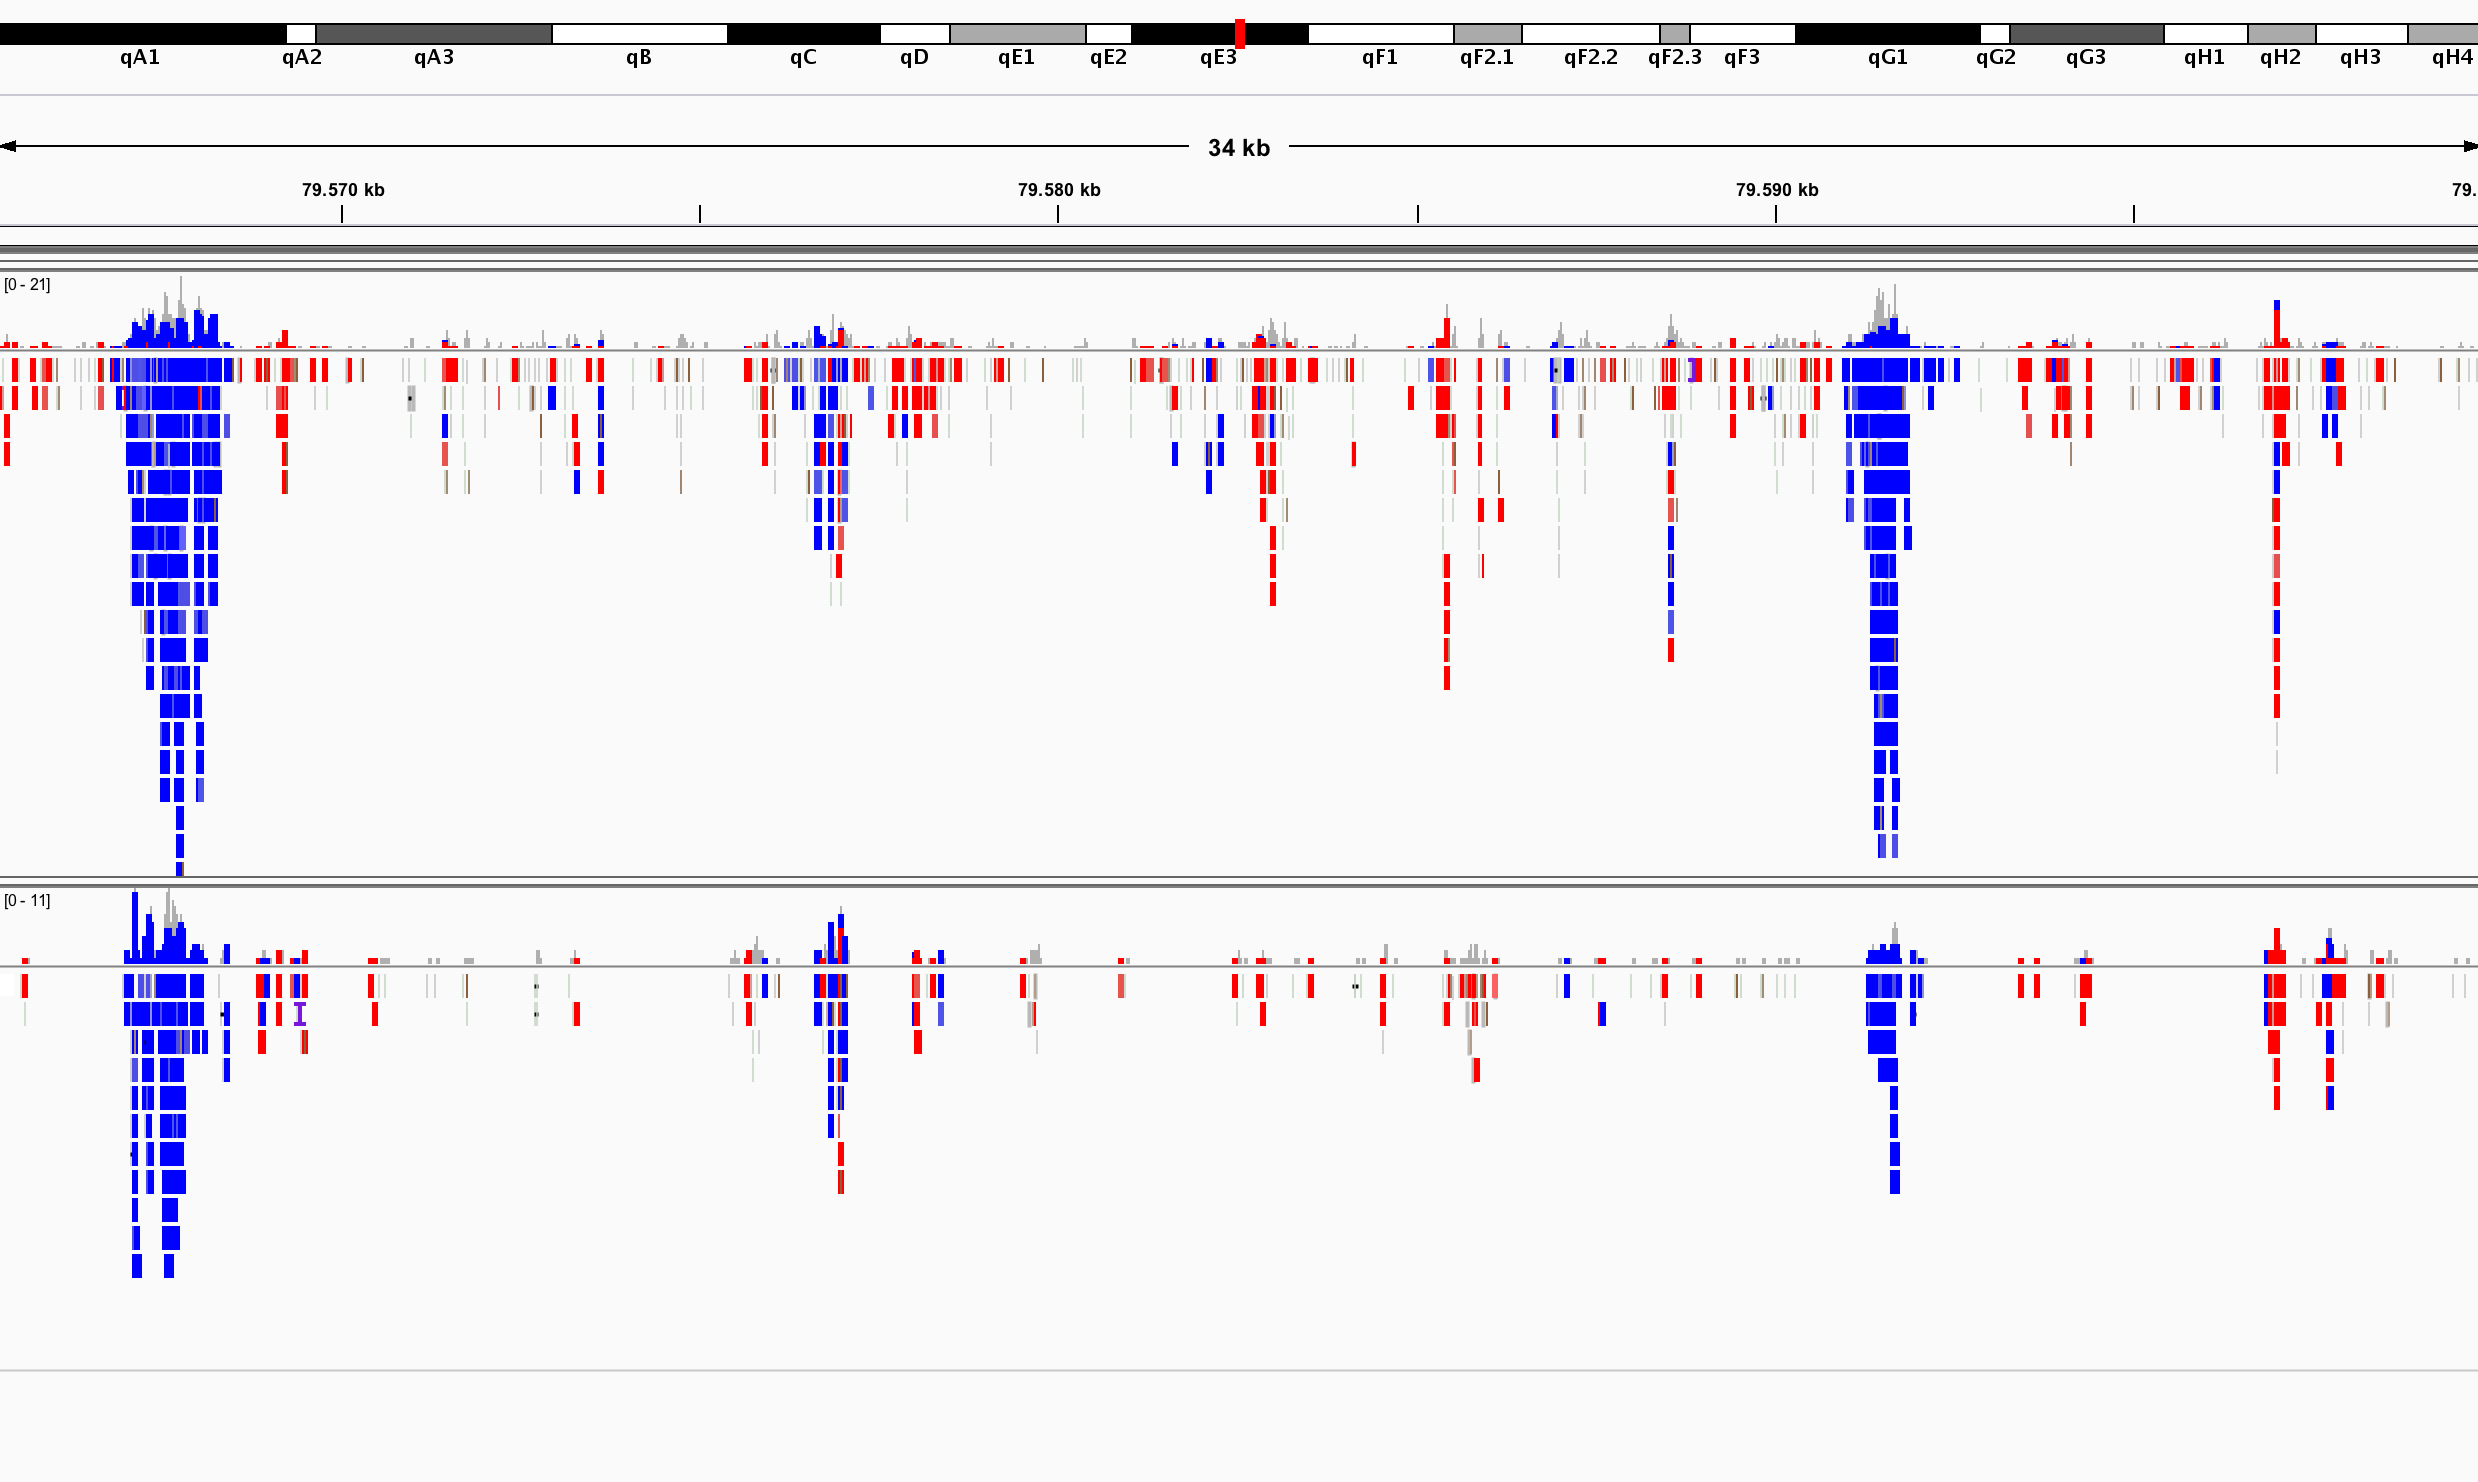
\includegraphics[scale=0.25, trim={0 0 0 16cm}, clip]{purifiedDNA.png}
  \end{figure}
  Mouse intestine, 100 cells
\end{frame}


\begin{frame}{Uneven coverage in scBS-seq data}
  \vspace{-0.2cm}
  \begin{figure}
      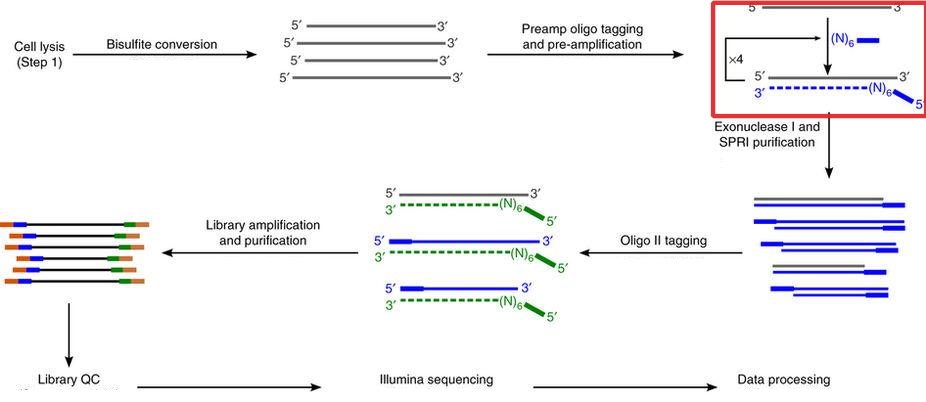
\includegraphics[scale=0.23]{wolf_reik_prot_preamp.png}
  \end{figure}
  \footlineextra{Clark et al. Nature Protocols 2017}
  \begin{figure}
      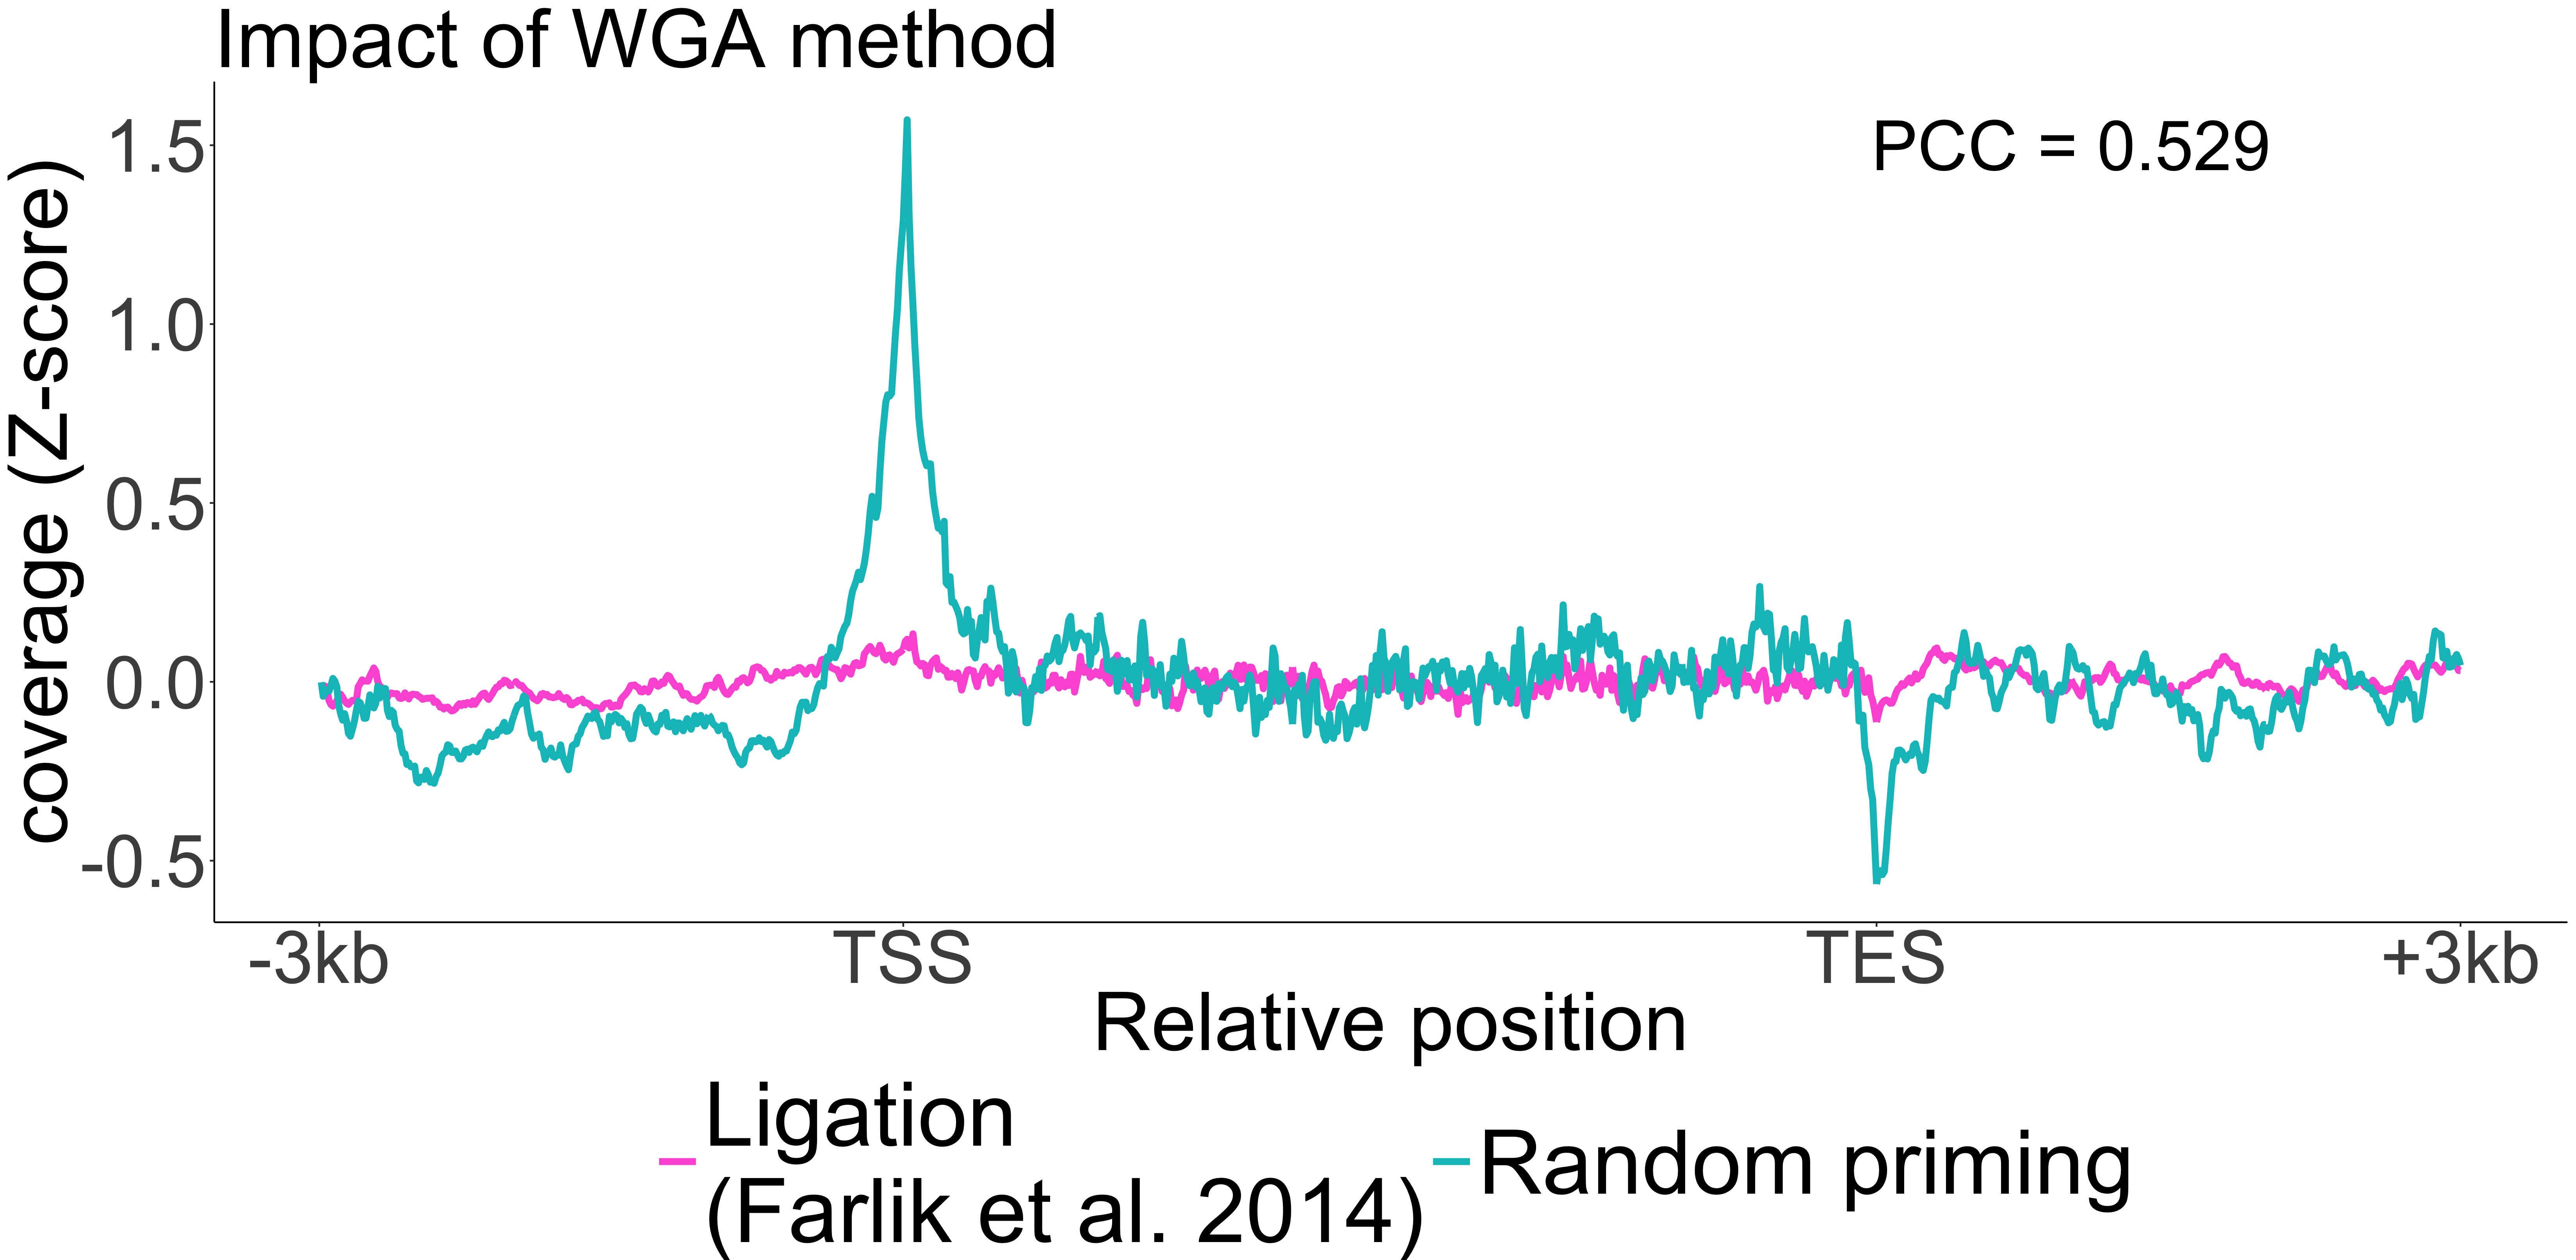
\includegraphics[scale = 0.03]{wga_bias.png}
  \end{figure}
\end{frame}

\begin{frame}{Modelling random hexamer binding}
  \vspace{-2cm}
  \begin{figure}
      \centering
      
\includegraphics[scale=0.25, trim={0 3cm 0 8cm}, clip]{template_primer.png}
  \end{figure}
\begin{figure}
  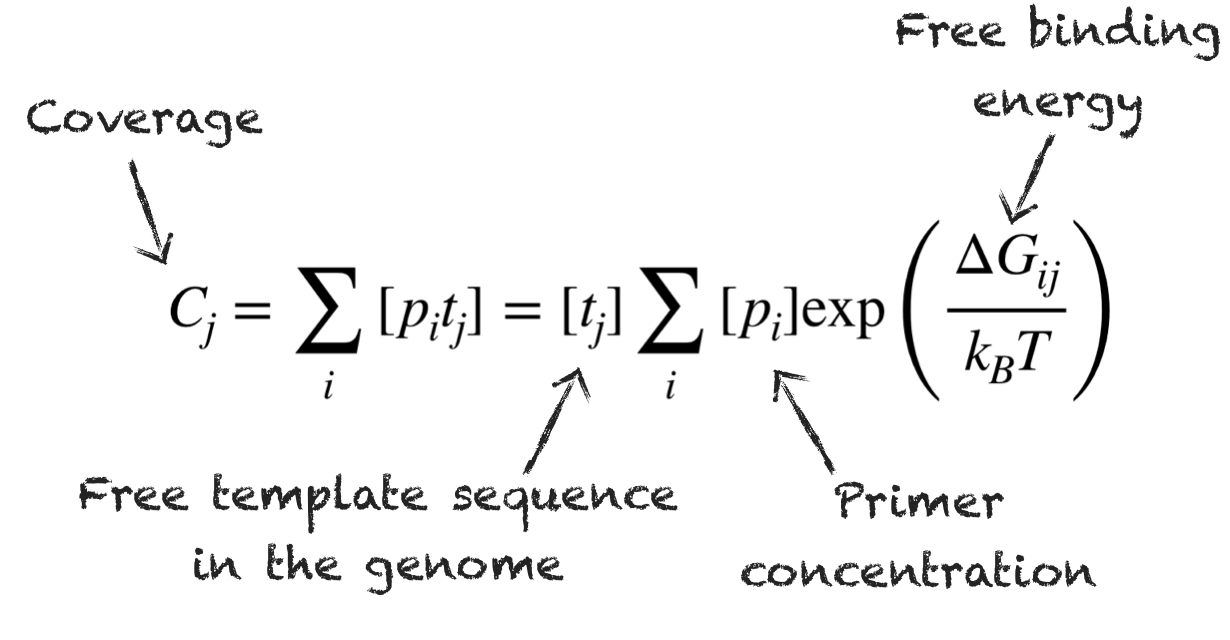
\includegraphics[scale=0.3]{model_w_labels.png}
\end{figure}
\begin{itemize}
  \item High frequency of mismatching primer-template events
  \item Lack of tabulated $\Delta$G values for non Watson-Crick base pairing
  \item Difficult to determine exact genomic kmer abundance for BS converted genome
\end{itemize}
\end{frame}

\begin{frame}{Outline}
    \tableofcontents
\end{frame}


\section{From sequence binding to genomic coverage profiles}

\begin{frame}{Does sequence binding explain genomic coverage profiles?}
  \begin{center}
    \textbf{Coverage fraction per sequence} \\
    $\downarrow$ \\
    \textbf{Coverage density per sequence} \\
    $\frac{kmer\ coverage}{kmer\ abundance}$ \\
    $\downarrow$ \\
    \textbf{Predicted coverage per position} \\
    sum of coverage densities for all sequences upstream 75 bp (read length)
  \end{center}
\end{frame}

\begin{frame}{Does sequence binding explain genomic coverage profiles?}
\vspace{-0.5cm}
\Wider{
\begin{columns}
    \begin{column}{0.5\linewidth}
      \begin{figure}
        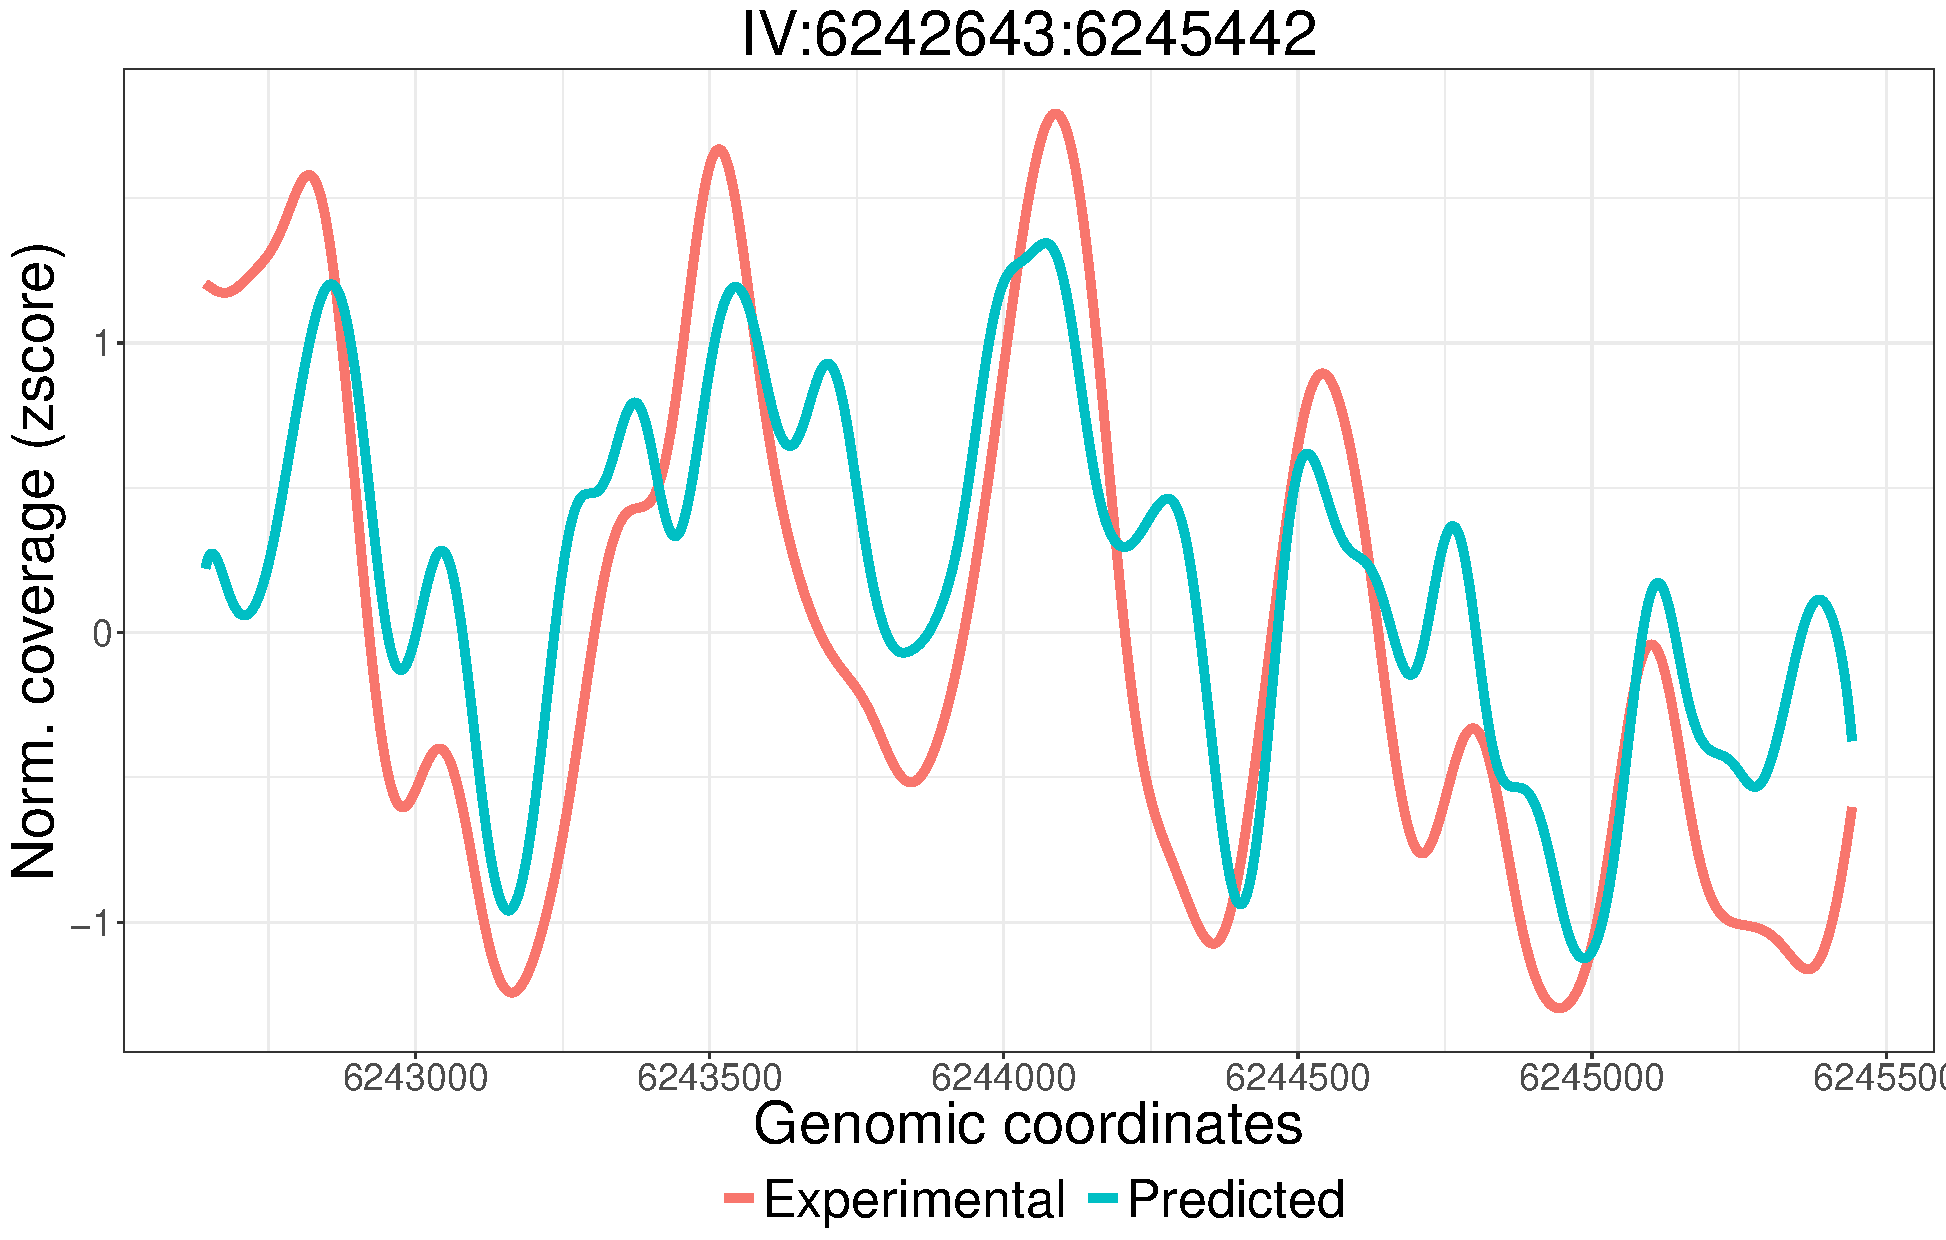
\includegraphics[scale=0.17]{highspear_celenoBS_smp1.pdf}
      \end{figure}
      \vspace{-0.7cm}
      \begin{figure}
        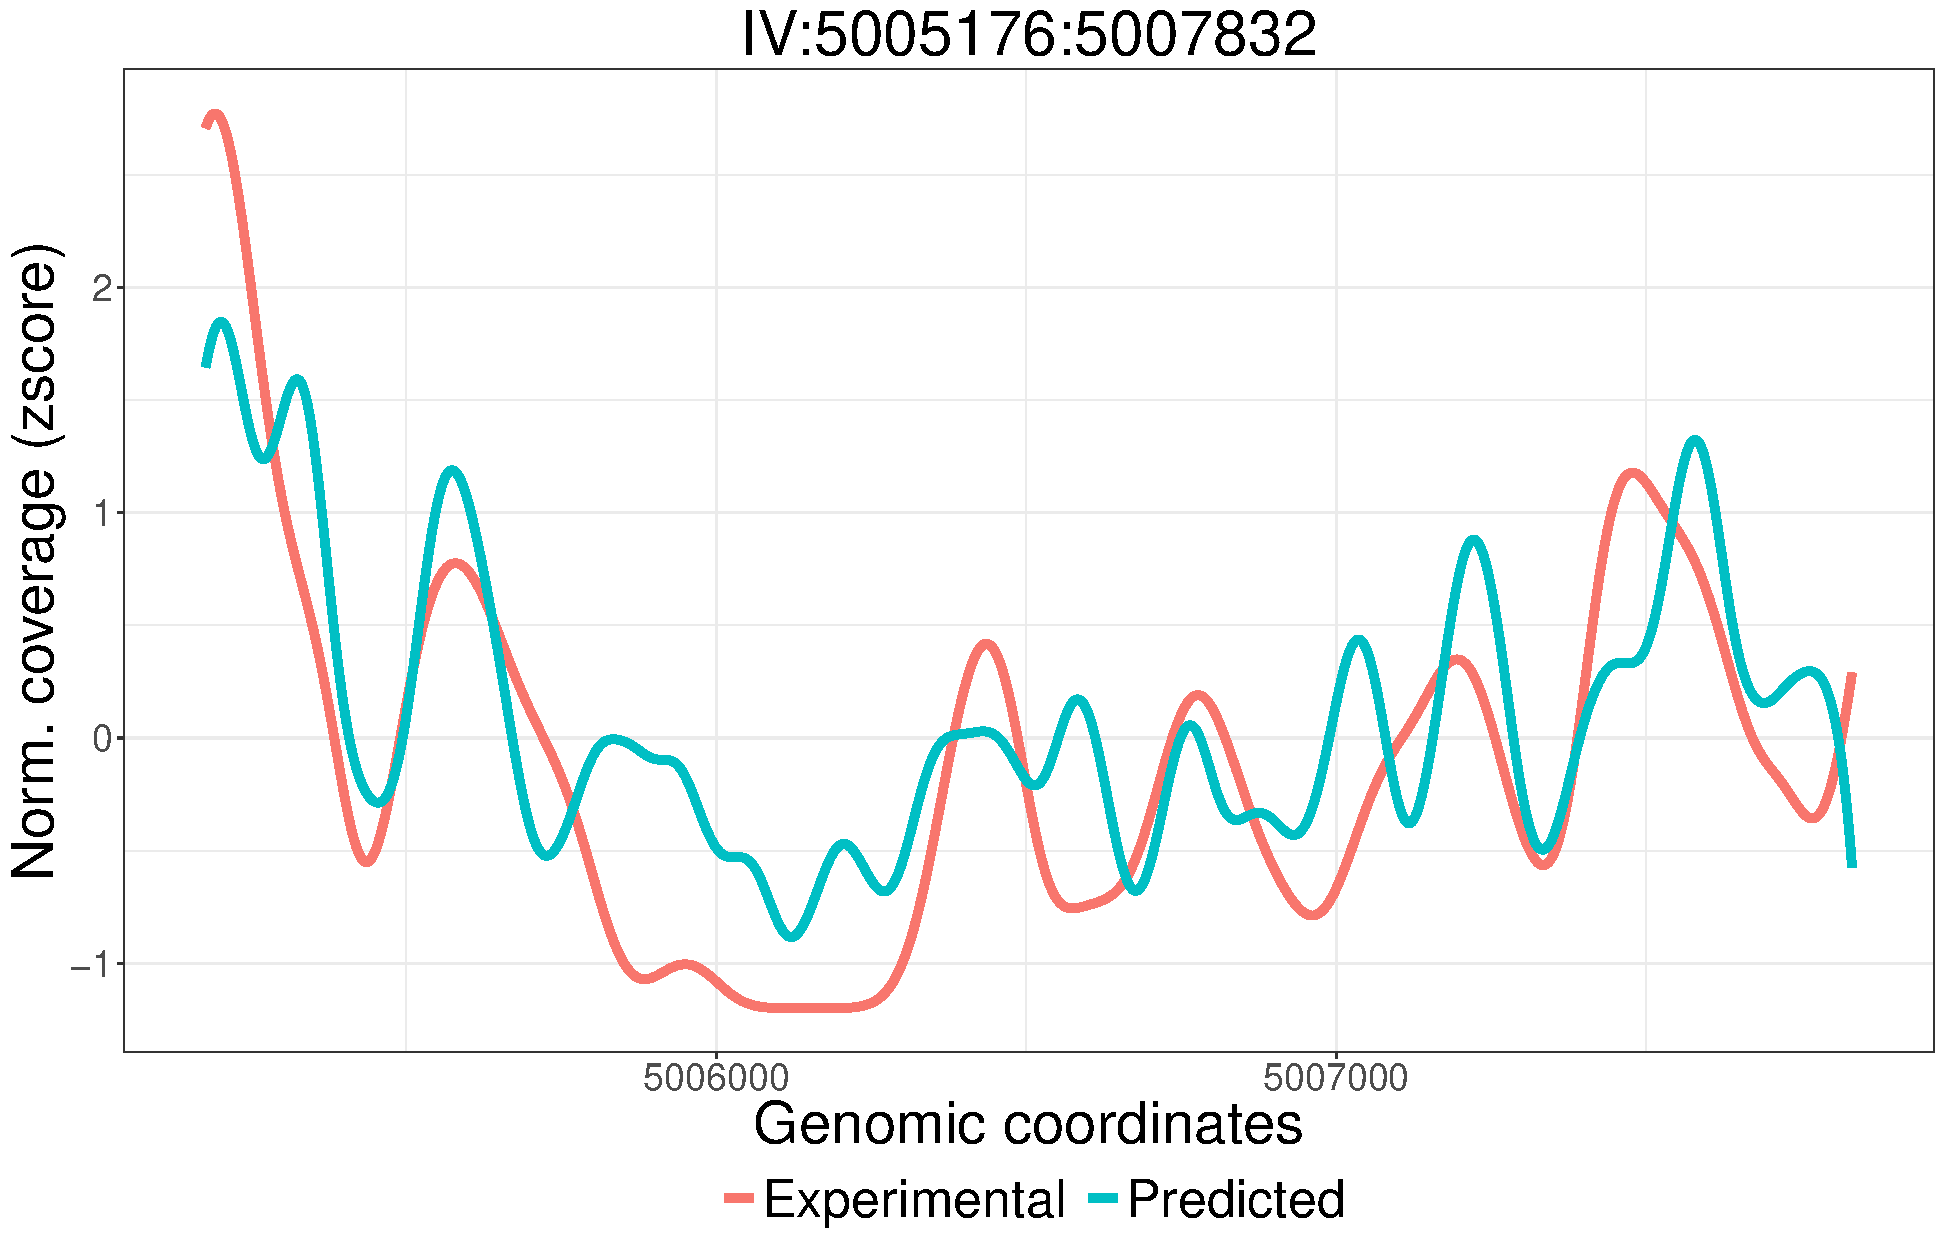
\includegraphics[scale=0.17]{highspear_celenoBS_smp2.pdf}
      \end{figure}
    \end{column}
    \begin{column}{0.5\linewidth}
      \begin{figure}
        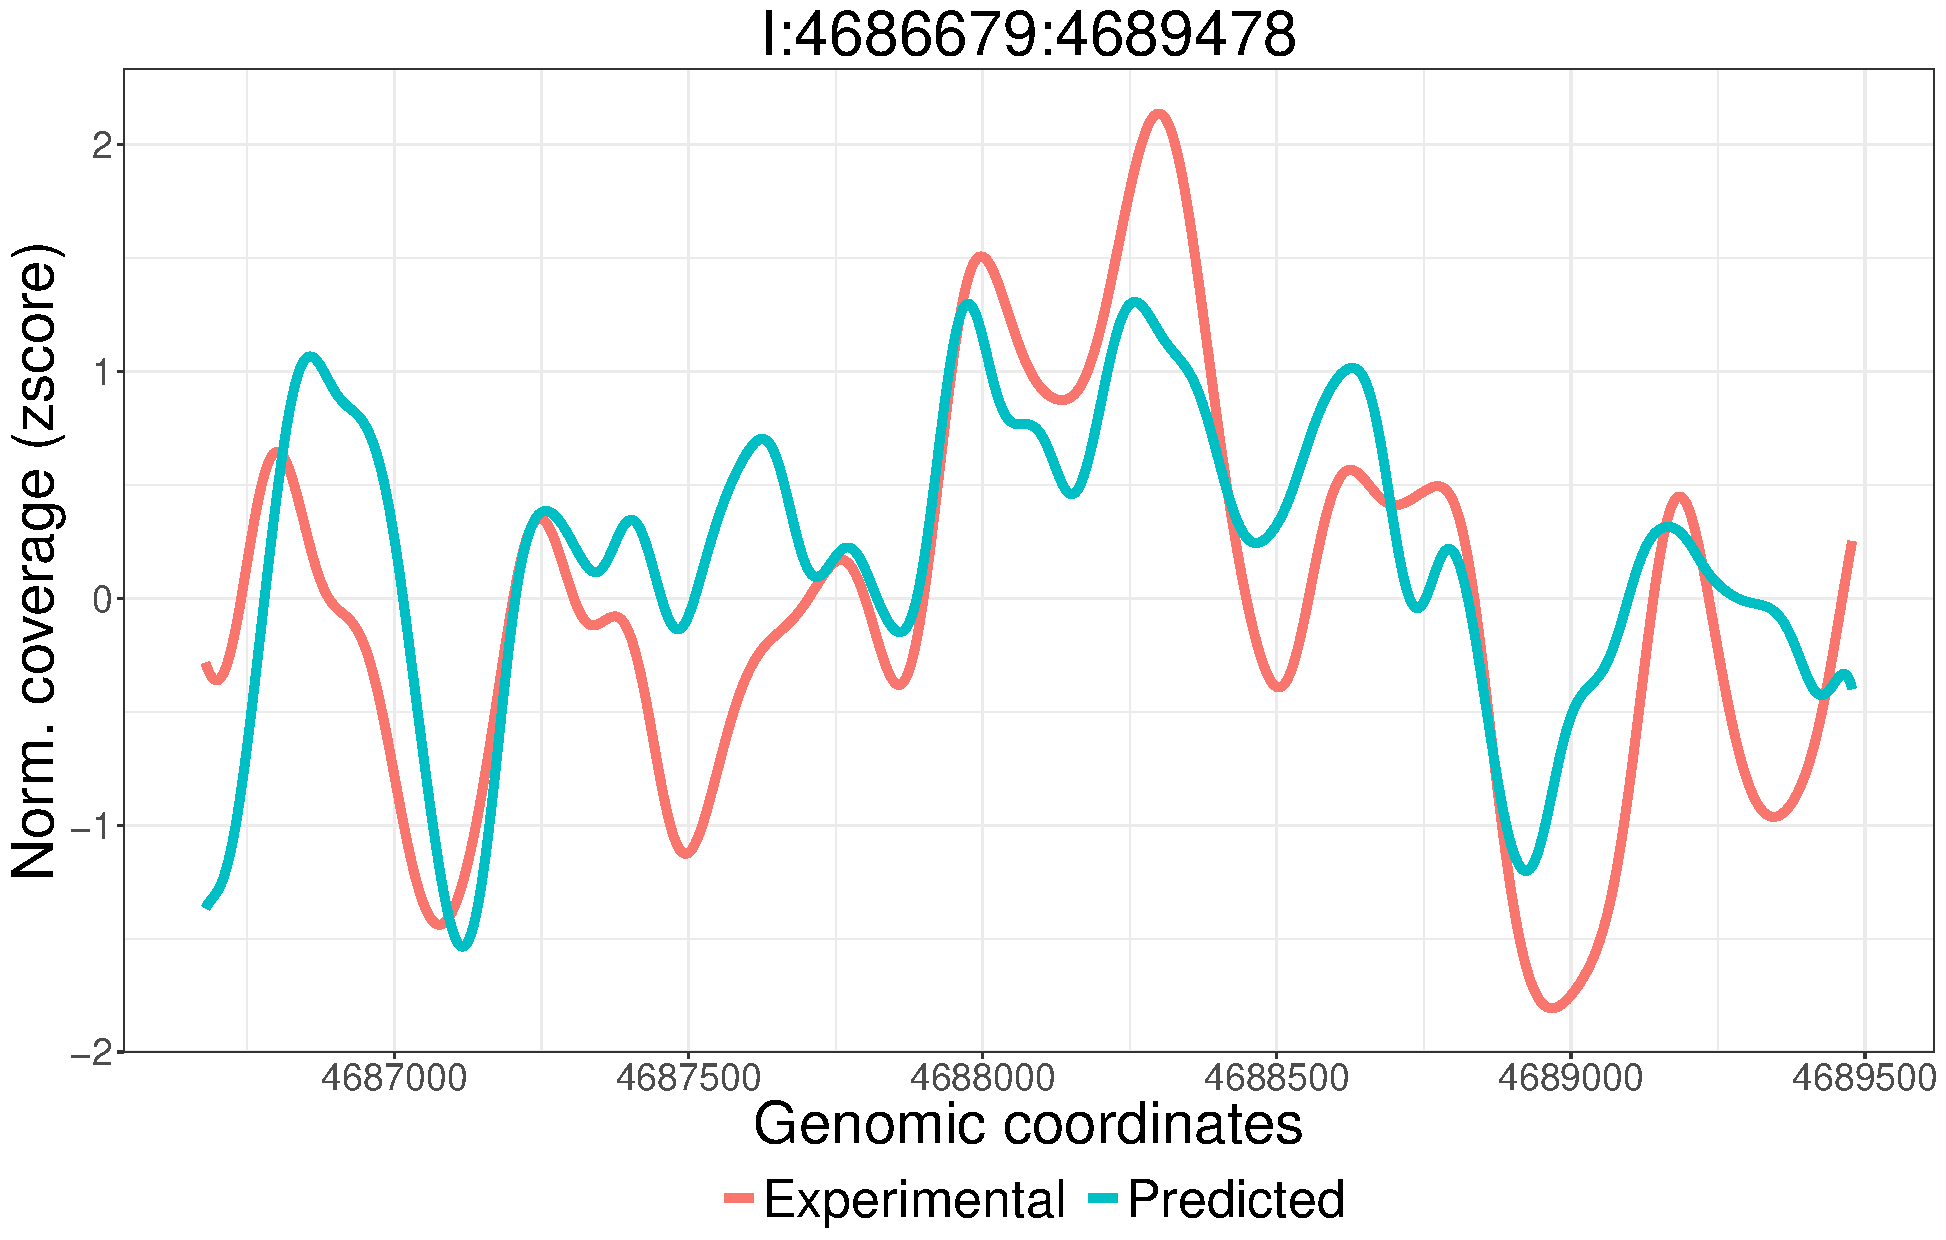
\includegraphics[scale=0.17]{highspear_celenoBS_smp3.pdf}
      \end{figure}
      \begin{figure}
        \vspace{-0.7cm}
        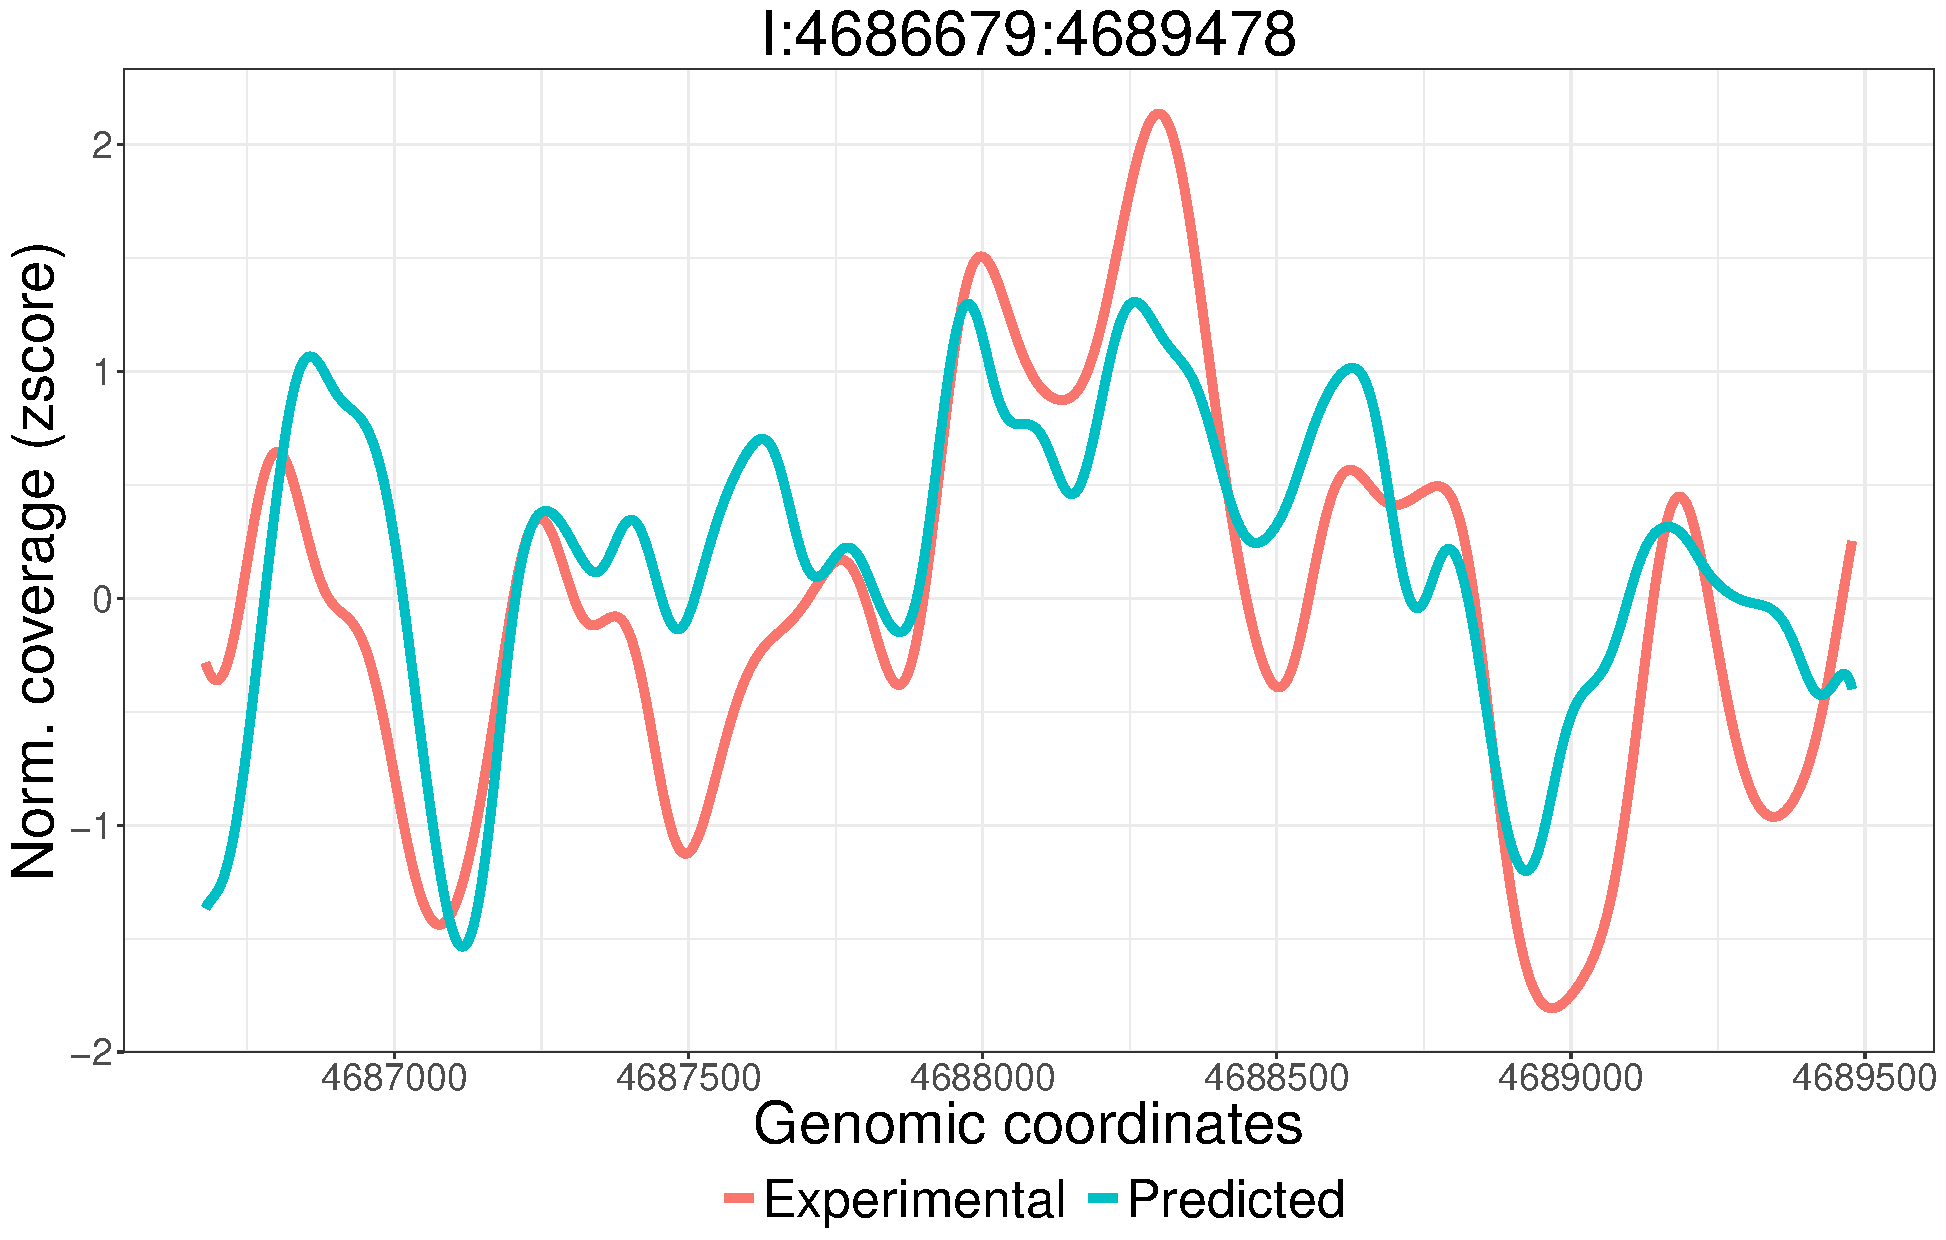
\includegraphics[scale=0.17]{highspear_celenoBS_smp3.pdf}
      \end{figure}
    \end{column}
  \end{columns}
  }
\end{frame}

\begin{frame}{Correlation between experimental and predicted coverage profiles}
  \Wider{
  \begin{columns}
      \begin{column}{0.4\linewidth}
        \begin{figure}
          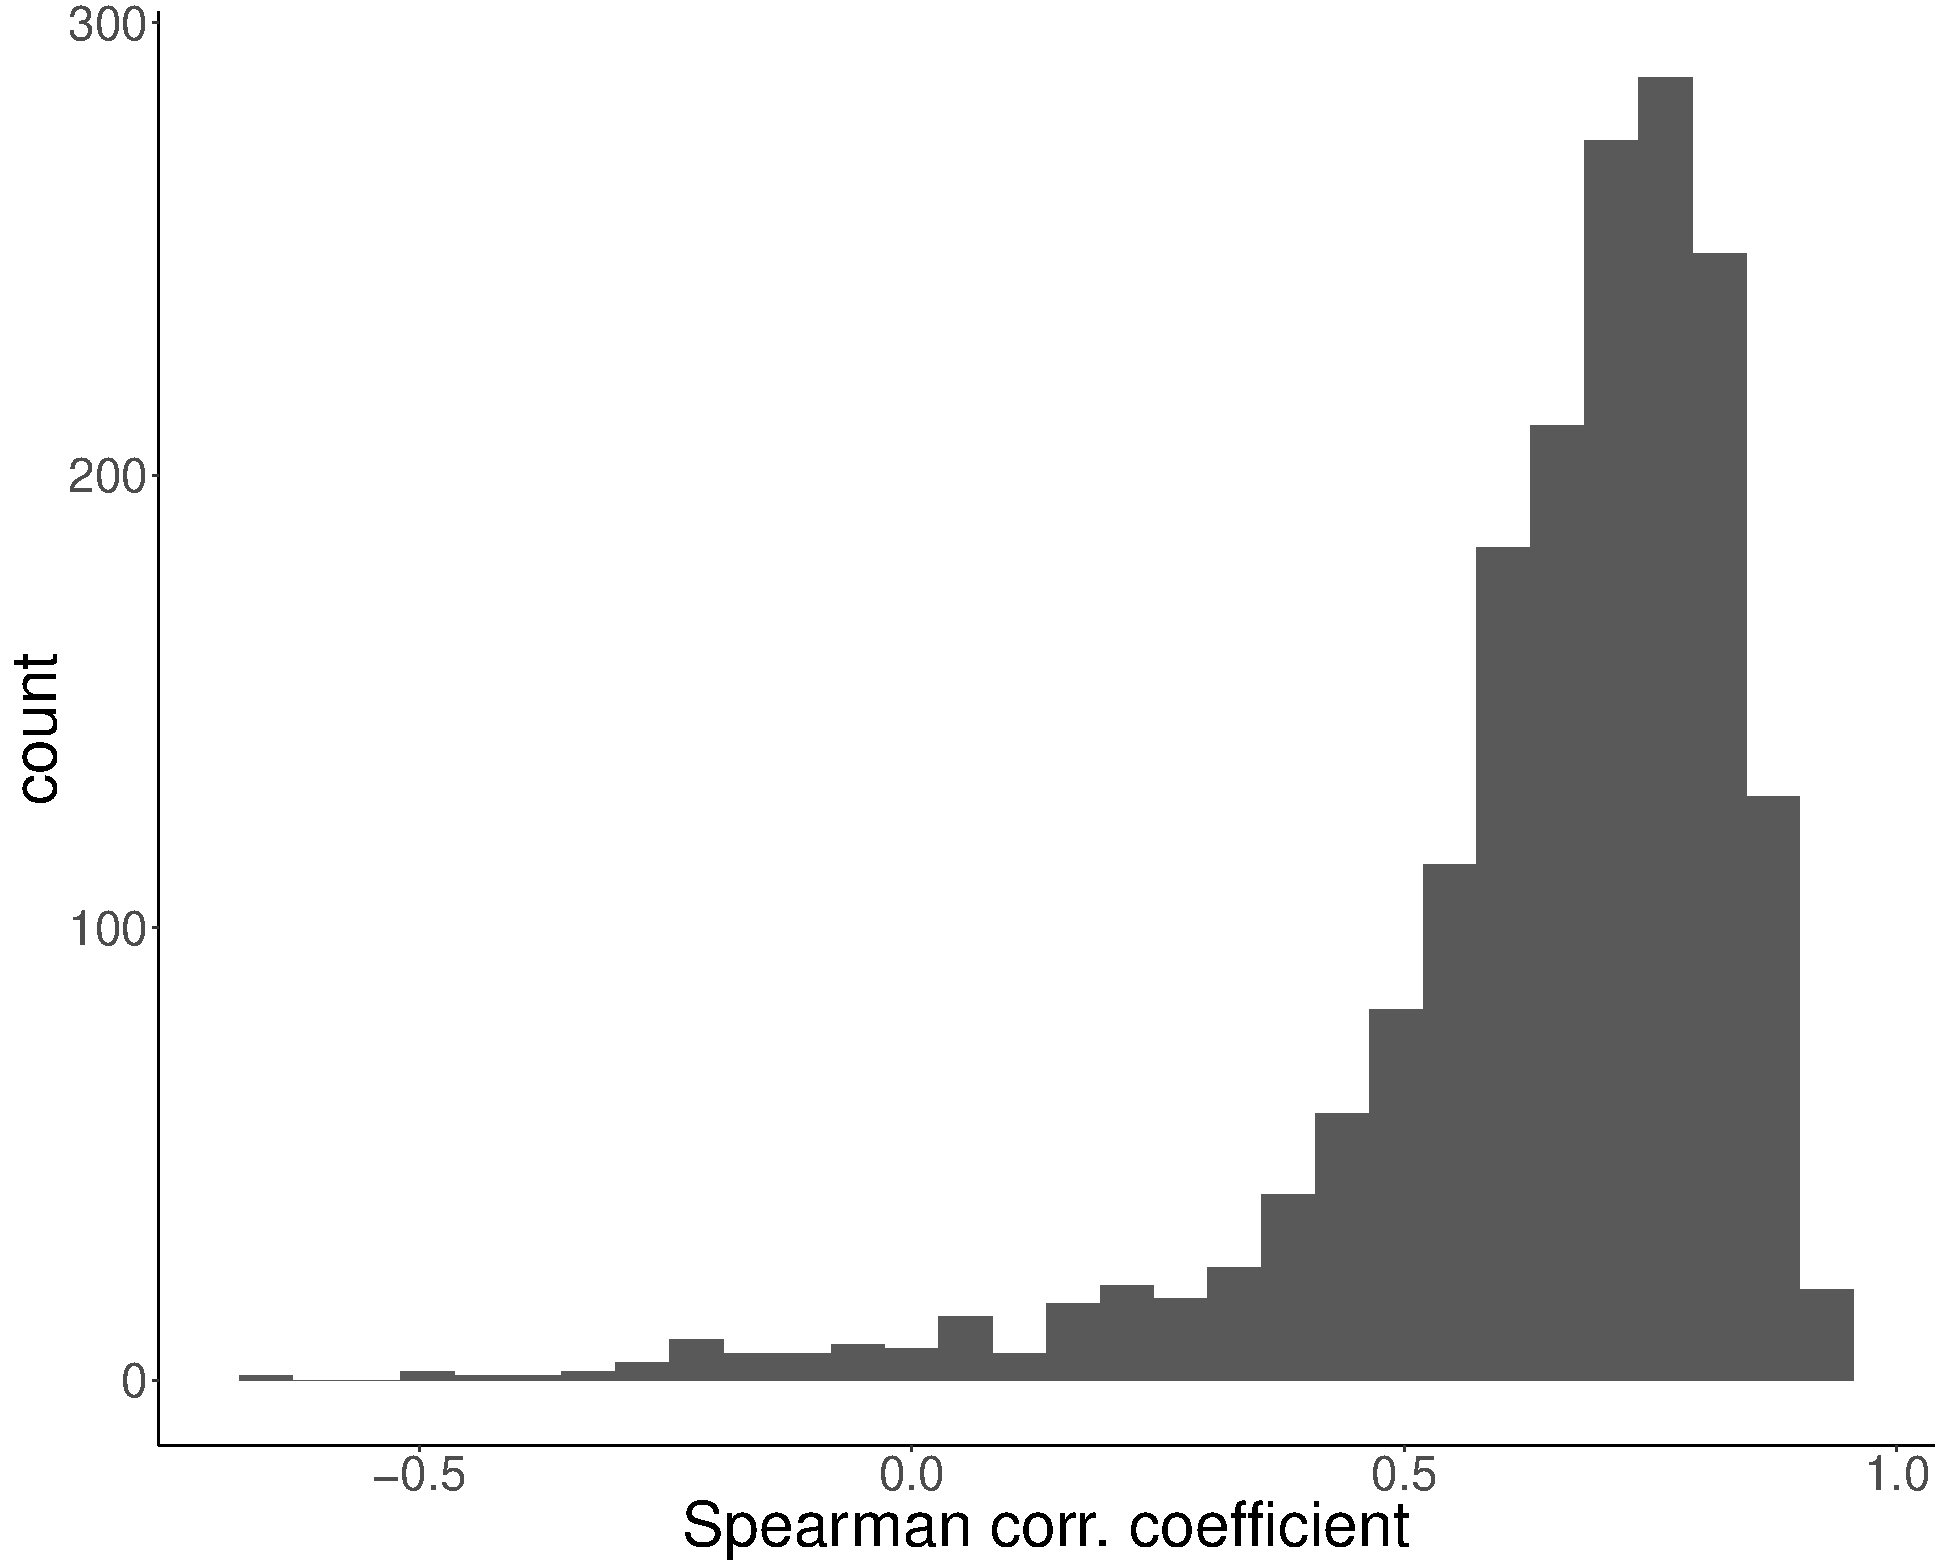
\includegraphics[scale=0.15]{spearman_distr_celeNoBS.pdf}
        \end{figure}
      \end{column}
      \begin{column}{0.55\linewidth}
        \begin{figure}
          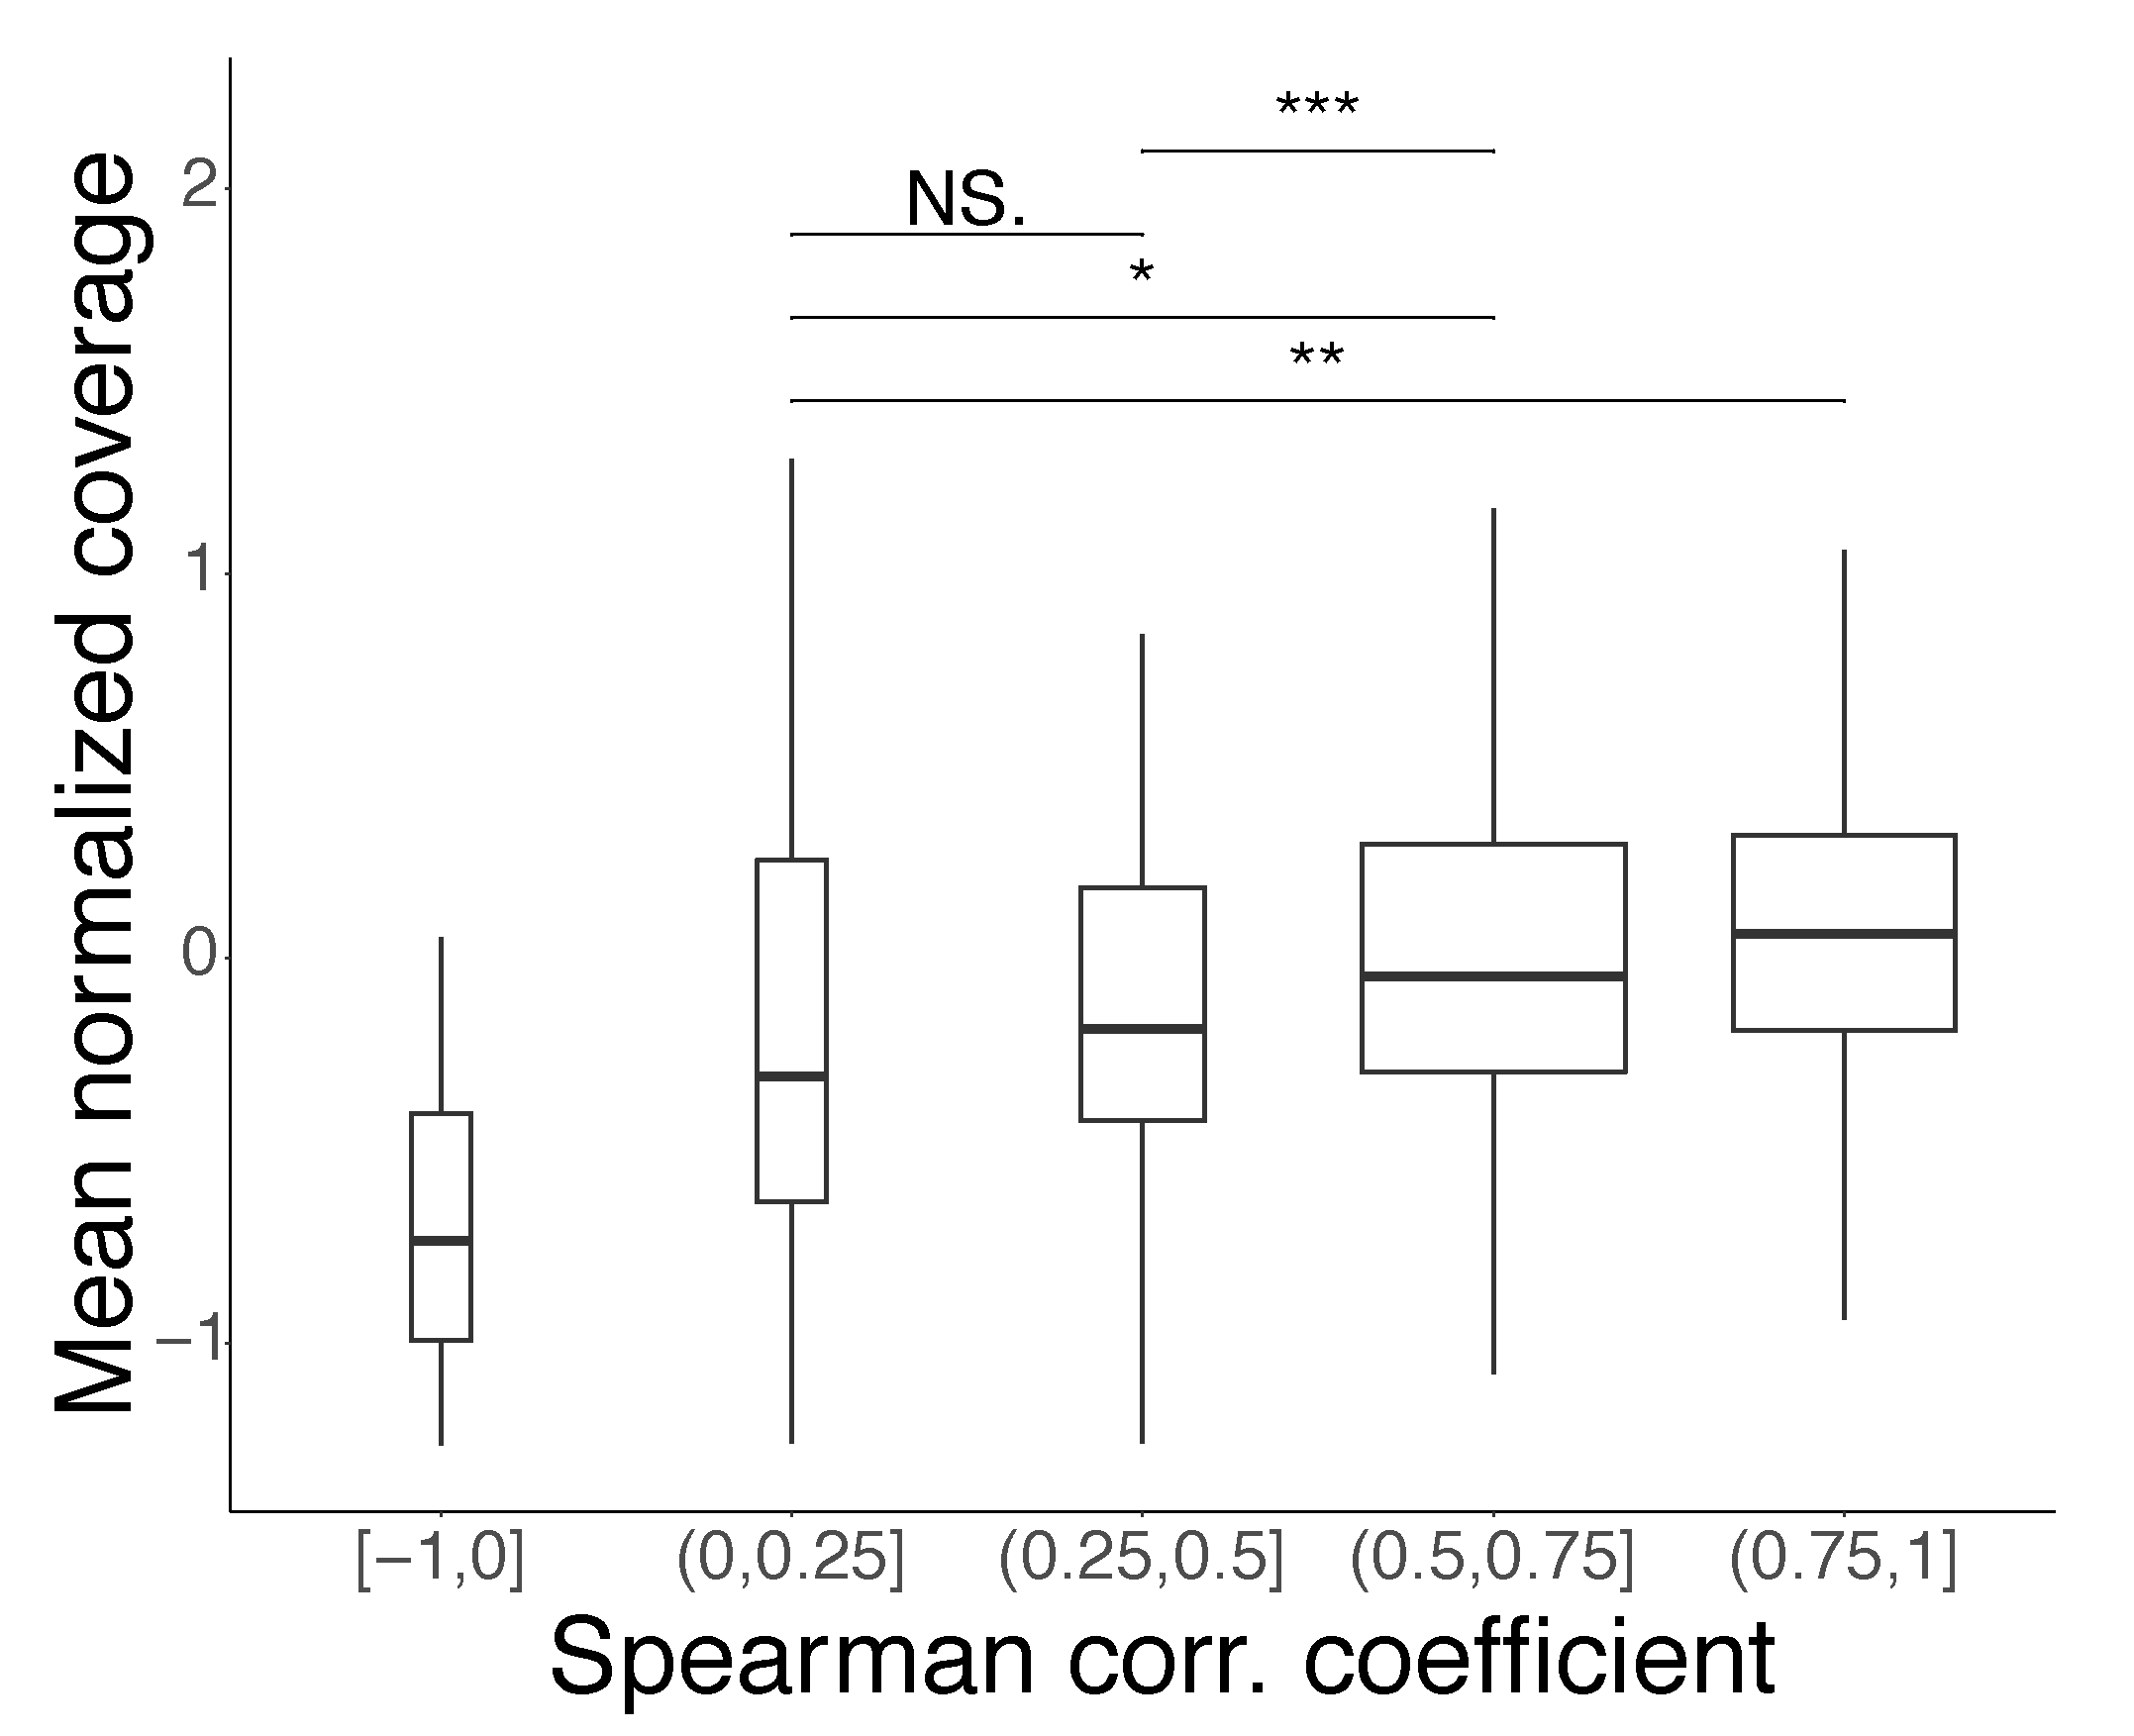
\includegraphics[scale=0.17]{spearman_outliars_celeNoBS.pdf}
        \end{figure}
      \end{column}
    \end{columns}
    }
\end{frame}

\section{Model validation}

\begin{frame}{Validation dataset}
  \begin{center}
    \begin{tabular}{r|c|c}
      & no BS & BS \\
      \hline
      \textit{C.elegans} & \checkmark & \checkmark \\
      \textit{D.rerio} & \checkmark & \checkmark \\
      \textit{M.musculus} & X & \checkmark \\
      \textit{H.sapiens} & \checkmark & \checkmark \\
      \hline
      \% Mapped & 90-96 & 40-63 \\
    \end{tabular}
  \end{center}
  \begin{itemize}
    \item Controlled genomic kmer abundance with no BS and one pre-amplification
    \item Consistency of predicted $\Delta$G between species with different genomic kmer abundance
    \item Correlation of predicted $\Delta$G with tabulated values from calorimetry
  \end{itemize}
\end{frame}

\begin{frame}{Model fitting for matching p-t pairs}
  \begin{figure}
    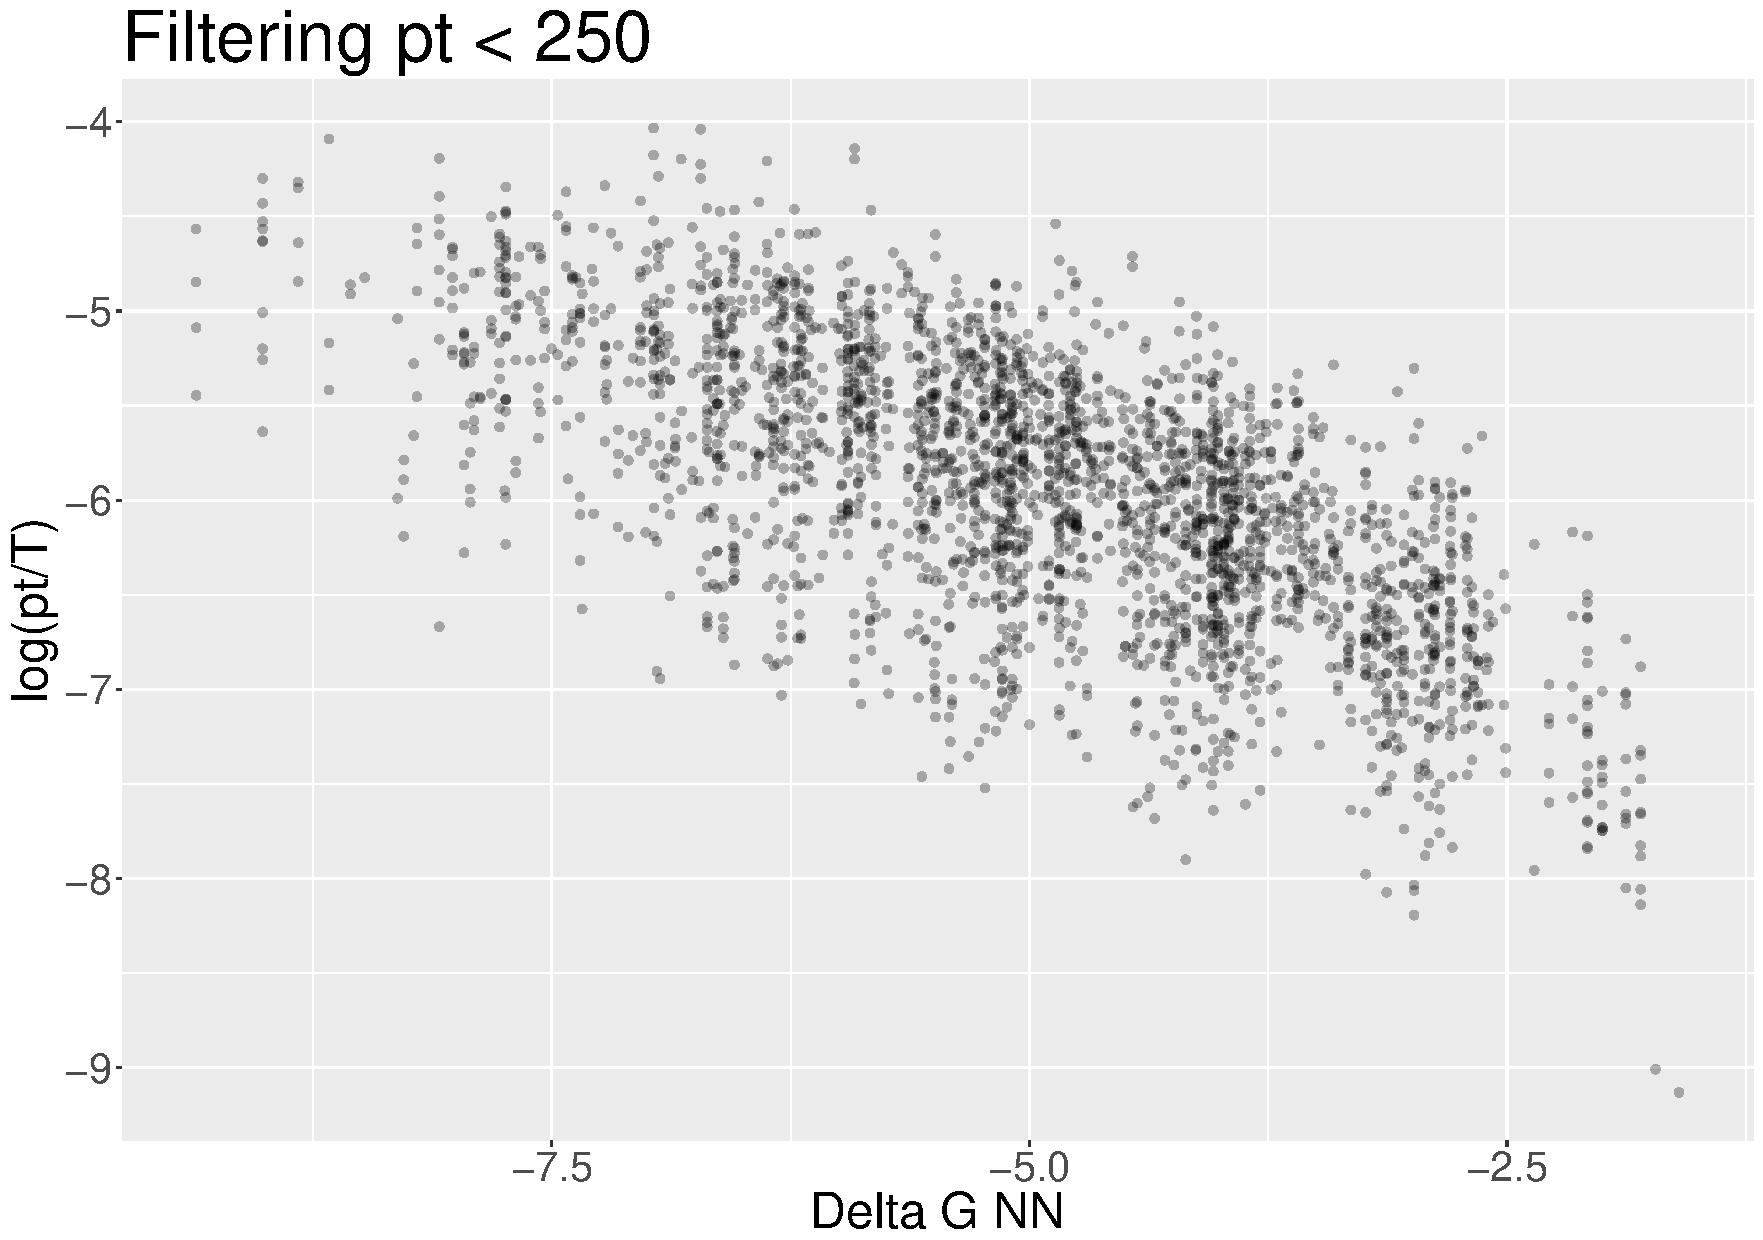
\includegraphics[scale=0.3]{model_fitting_zf_noBS_diag.pdf}
  \end{figure}
  \footlineextra{D.rerio - no BS}
\end{frame}

\begin{frame}{Consistency of $\Delta$G across genomes}
  % \Wider{
  \begin{figure}
    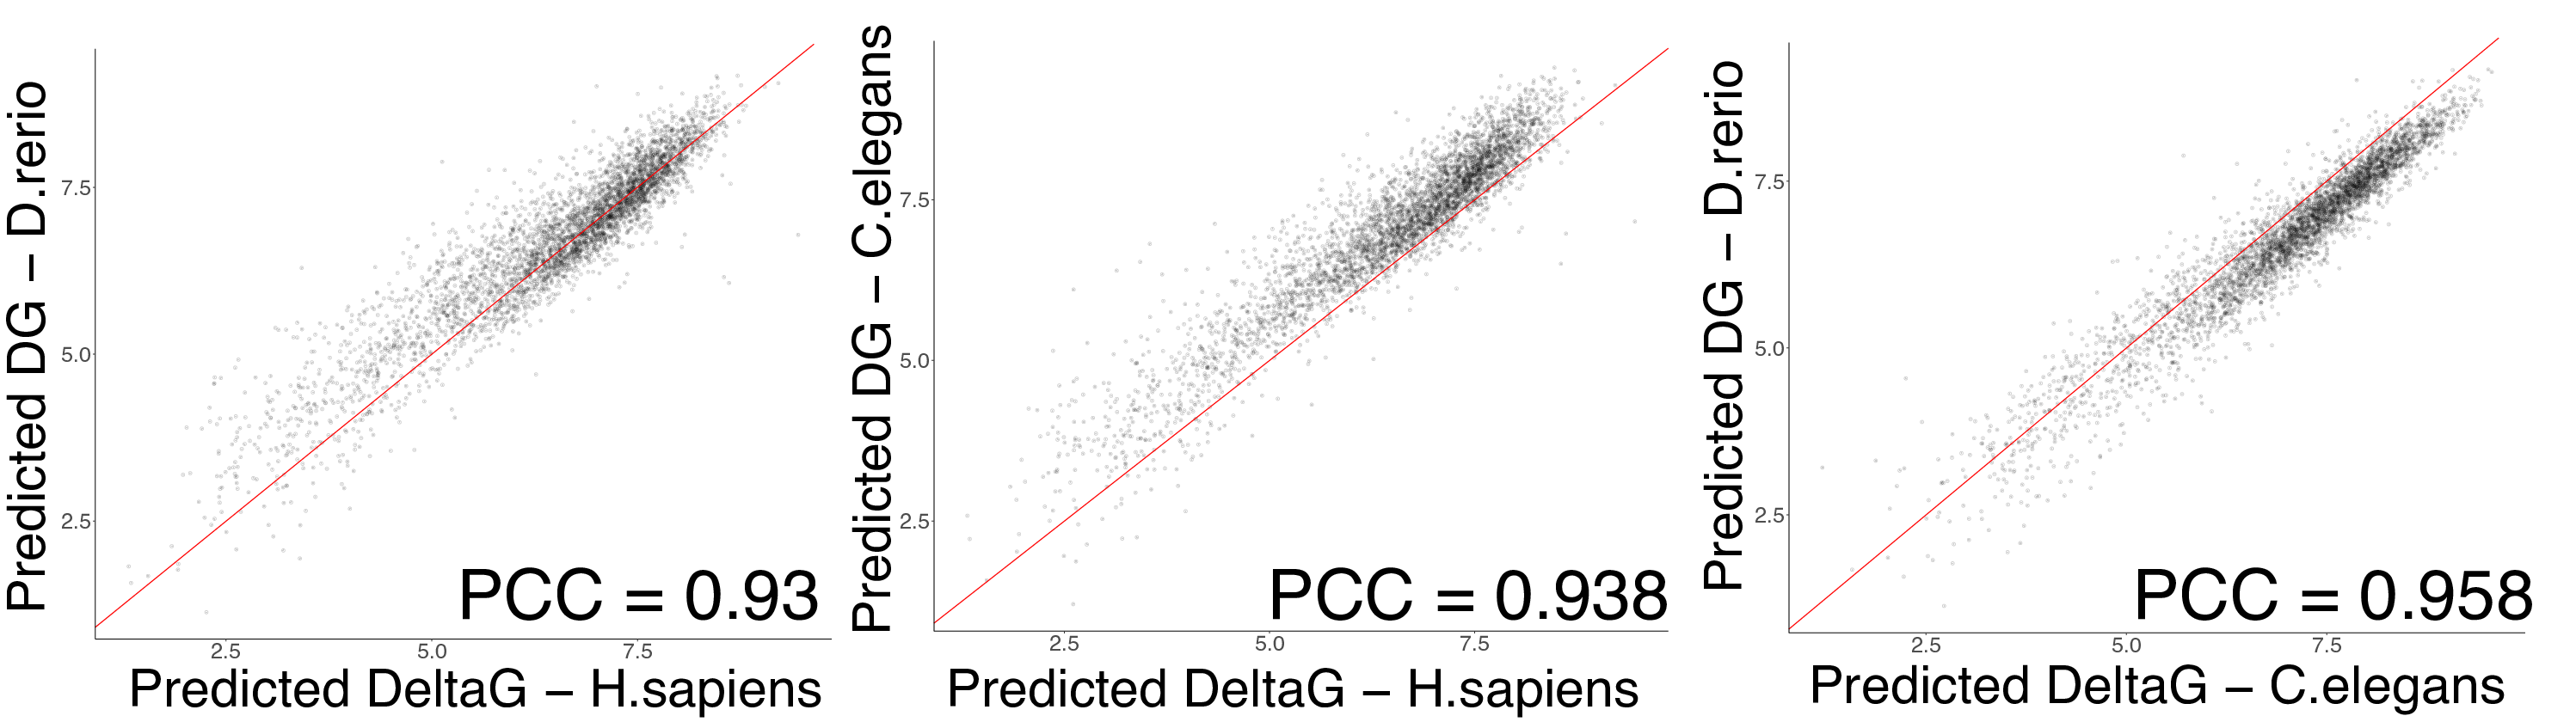
\includegraphics[scale=0.11]{deltaG_celVShuman_diag.png}
  \end{figure}
  Matching p-t pairs
  % }
\end{frame}

\begin{frame}{Consistency of $\Delta$G across genomes}
  % \Wider{
  \begin{figure}
    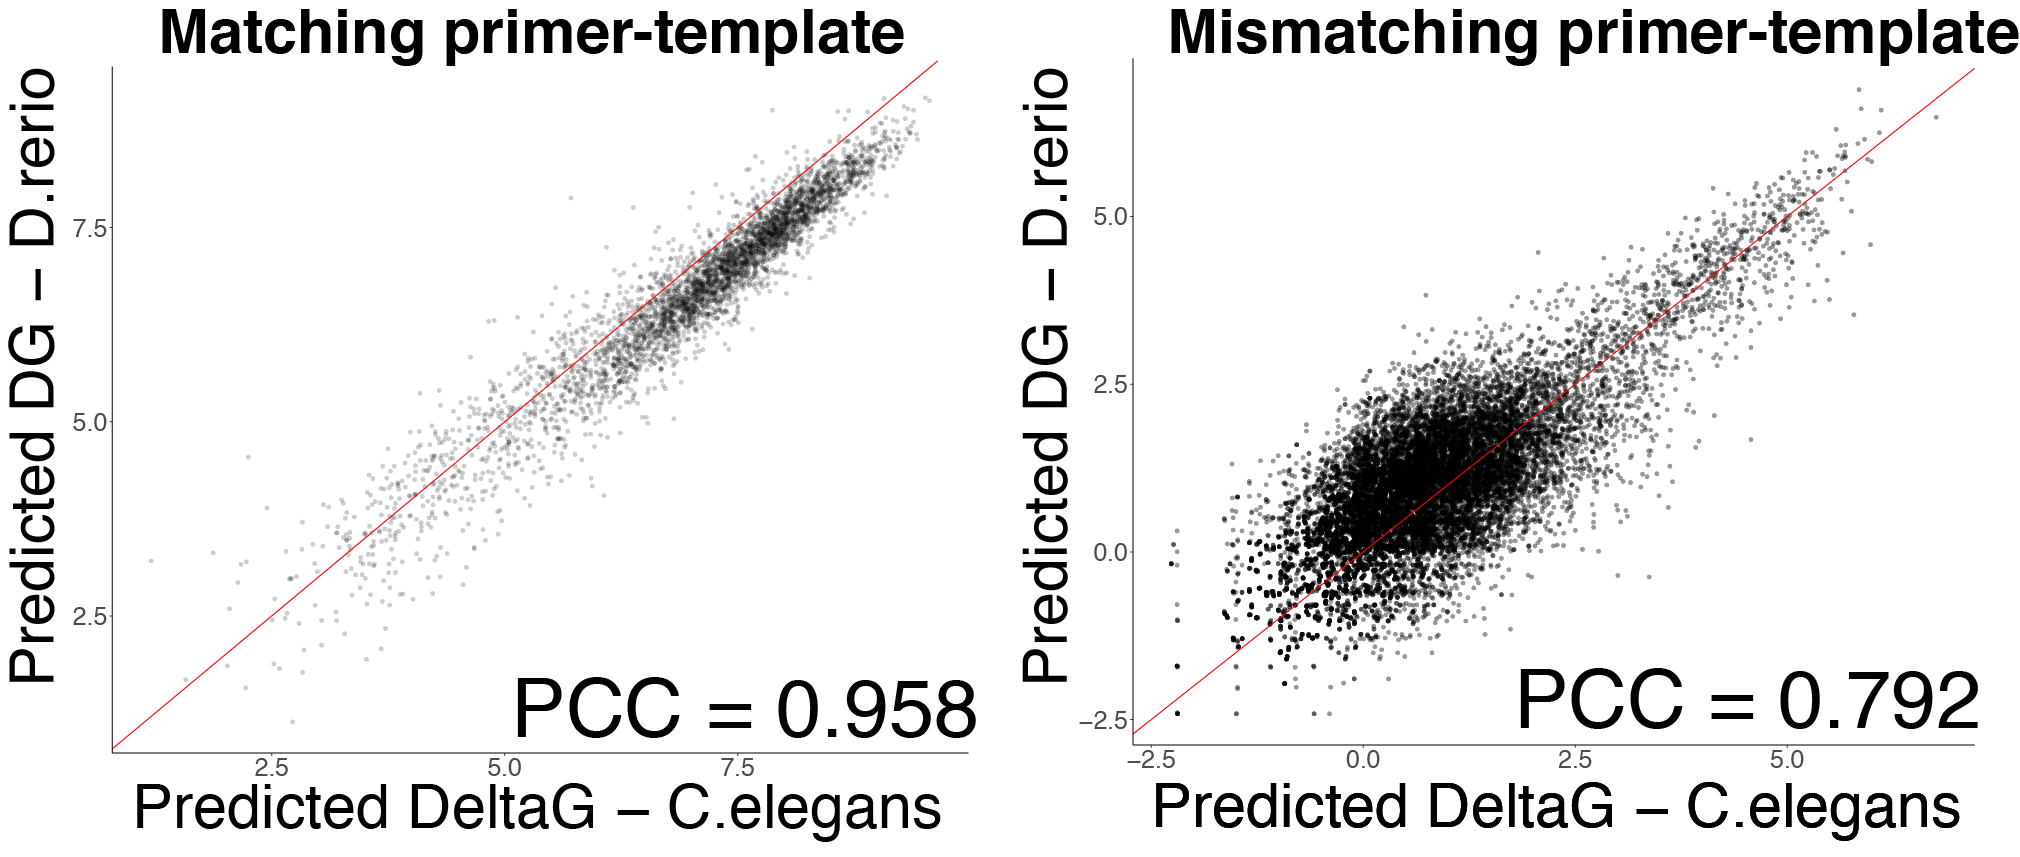
\includegraphics[scale=0.15]{deltaG_zfVScele_matchingNmismatching_filt200counts.png}
  \end{figure}
  % }
\end{frame}

\begin{frame}{Correlation of $\Delta$G with tabulated values}
  % \Wider{
  \begin{figure}
    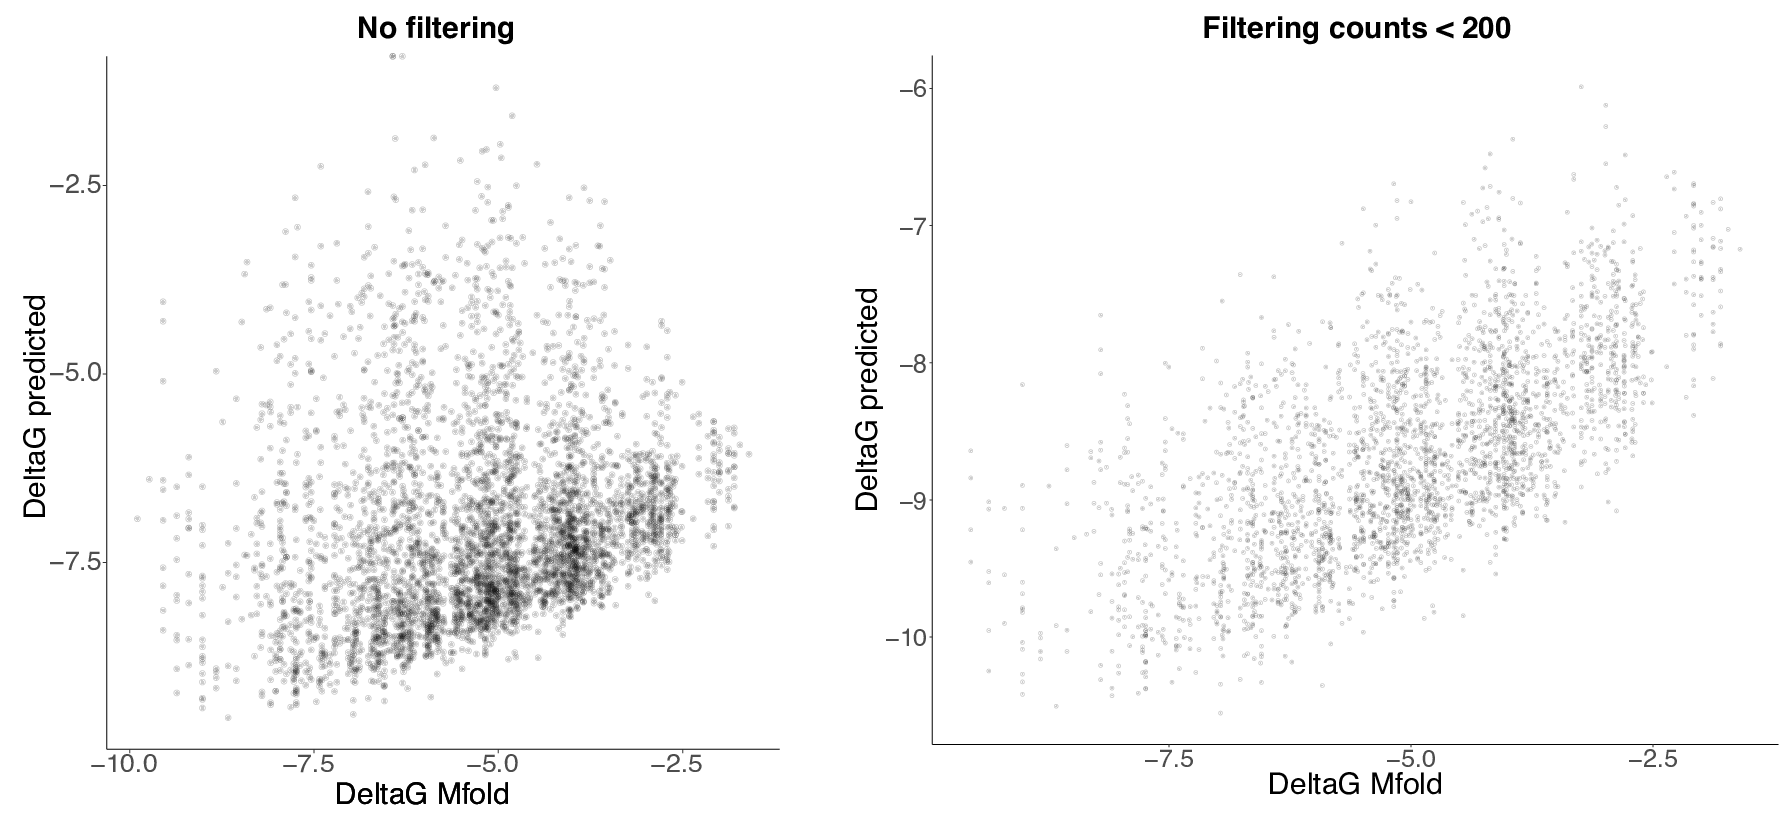
\includegraphics[scale=0.23, trim={28cm 0 0 0}, clip]{deltaG_celeVSmfold_filt200counts.pdf}
  \end{figure}
  % }
\end{frame}

\section{Optimizing the primer pool}

\begin{frame}{How does primer concentration affect coverage?}
  \vspace{-0.8cm}
  \begin{figure}
    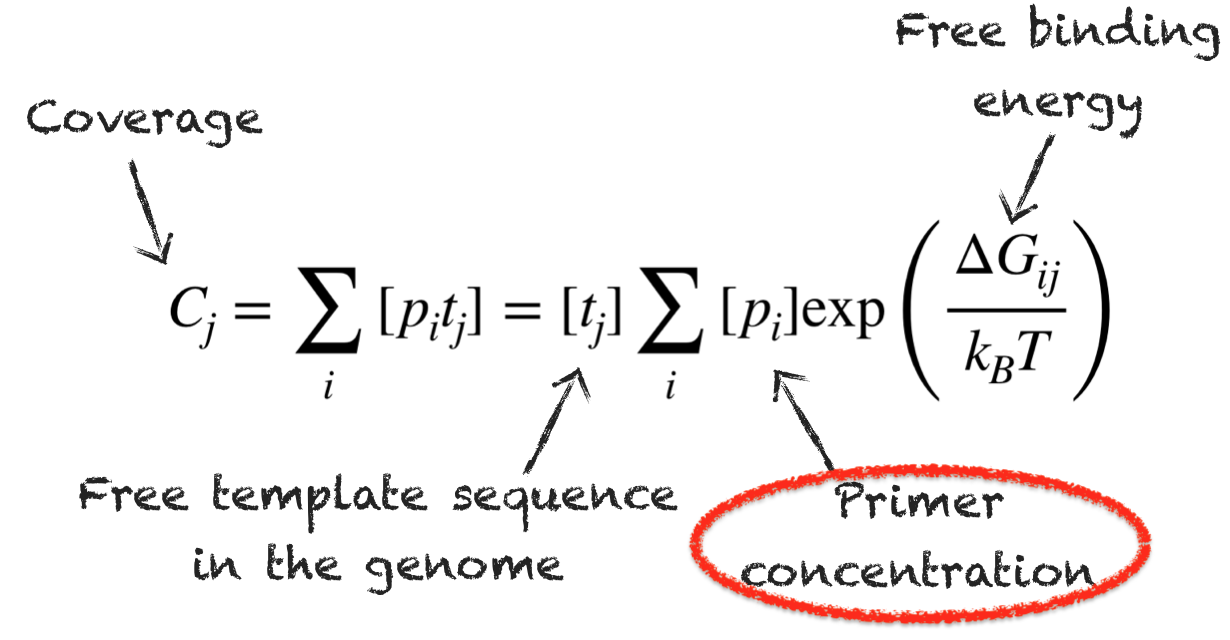
\includegraphics[scale=0.23]{model_w_labels_primer_mark.png}
  \end{figure}
  \only<1>{Primer batch composition}
  \only<2>{Primer usage}
  \only<3>{Template usage}
  \smallskip
% \Wider{
  \begin{columns}
    \begin{column}{0.3\linewidth}
      \centering{
      R = random
      \vspace{-0.2cm}
      \begin{figure}
      \only<1>{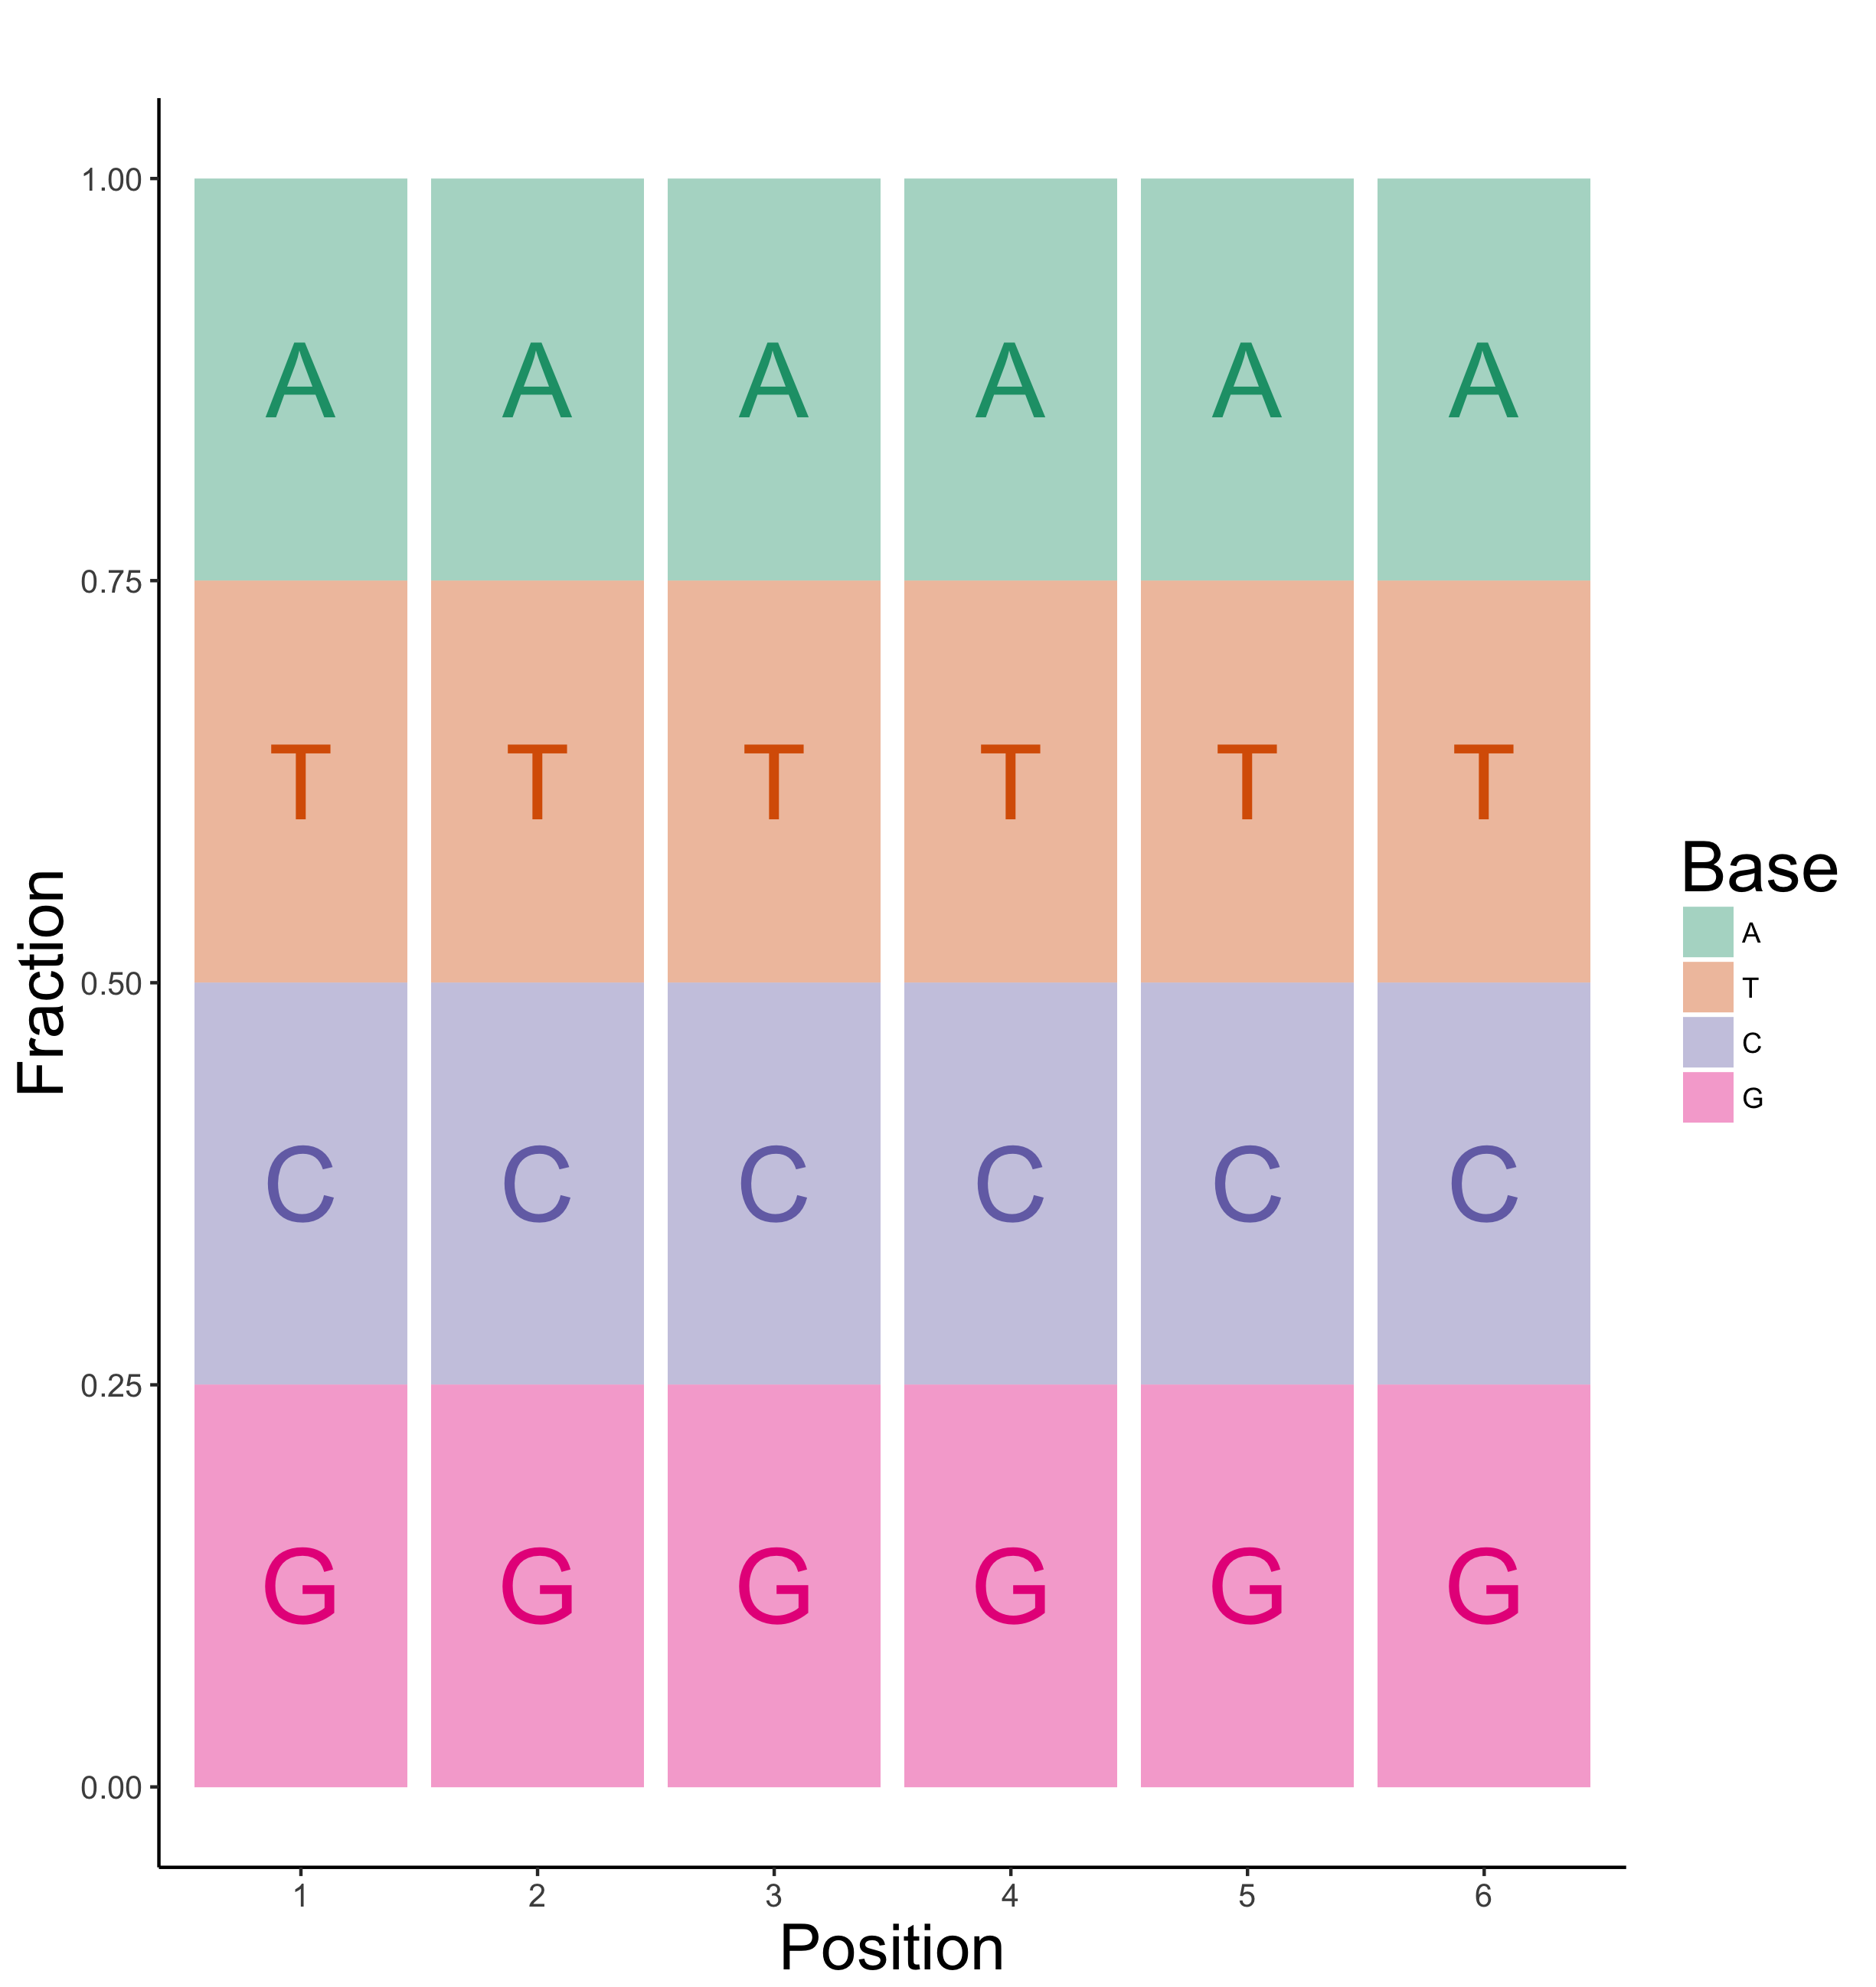
\includegraphics[scale=0.04, trim={0 0 9cm 7cm}, clip]{ppm_R.png}}
      \only<2>{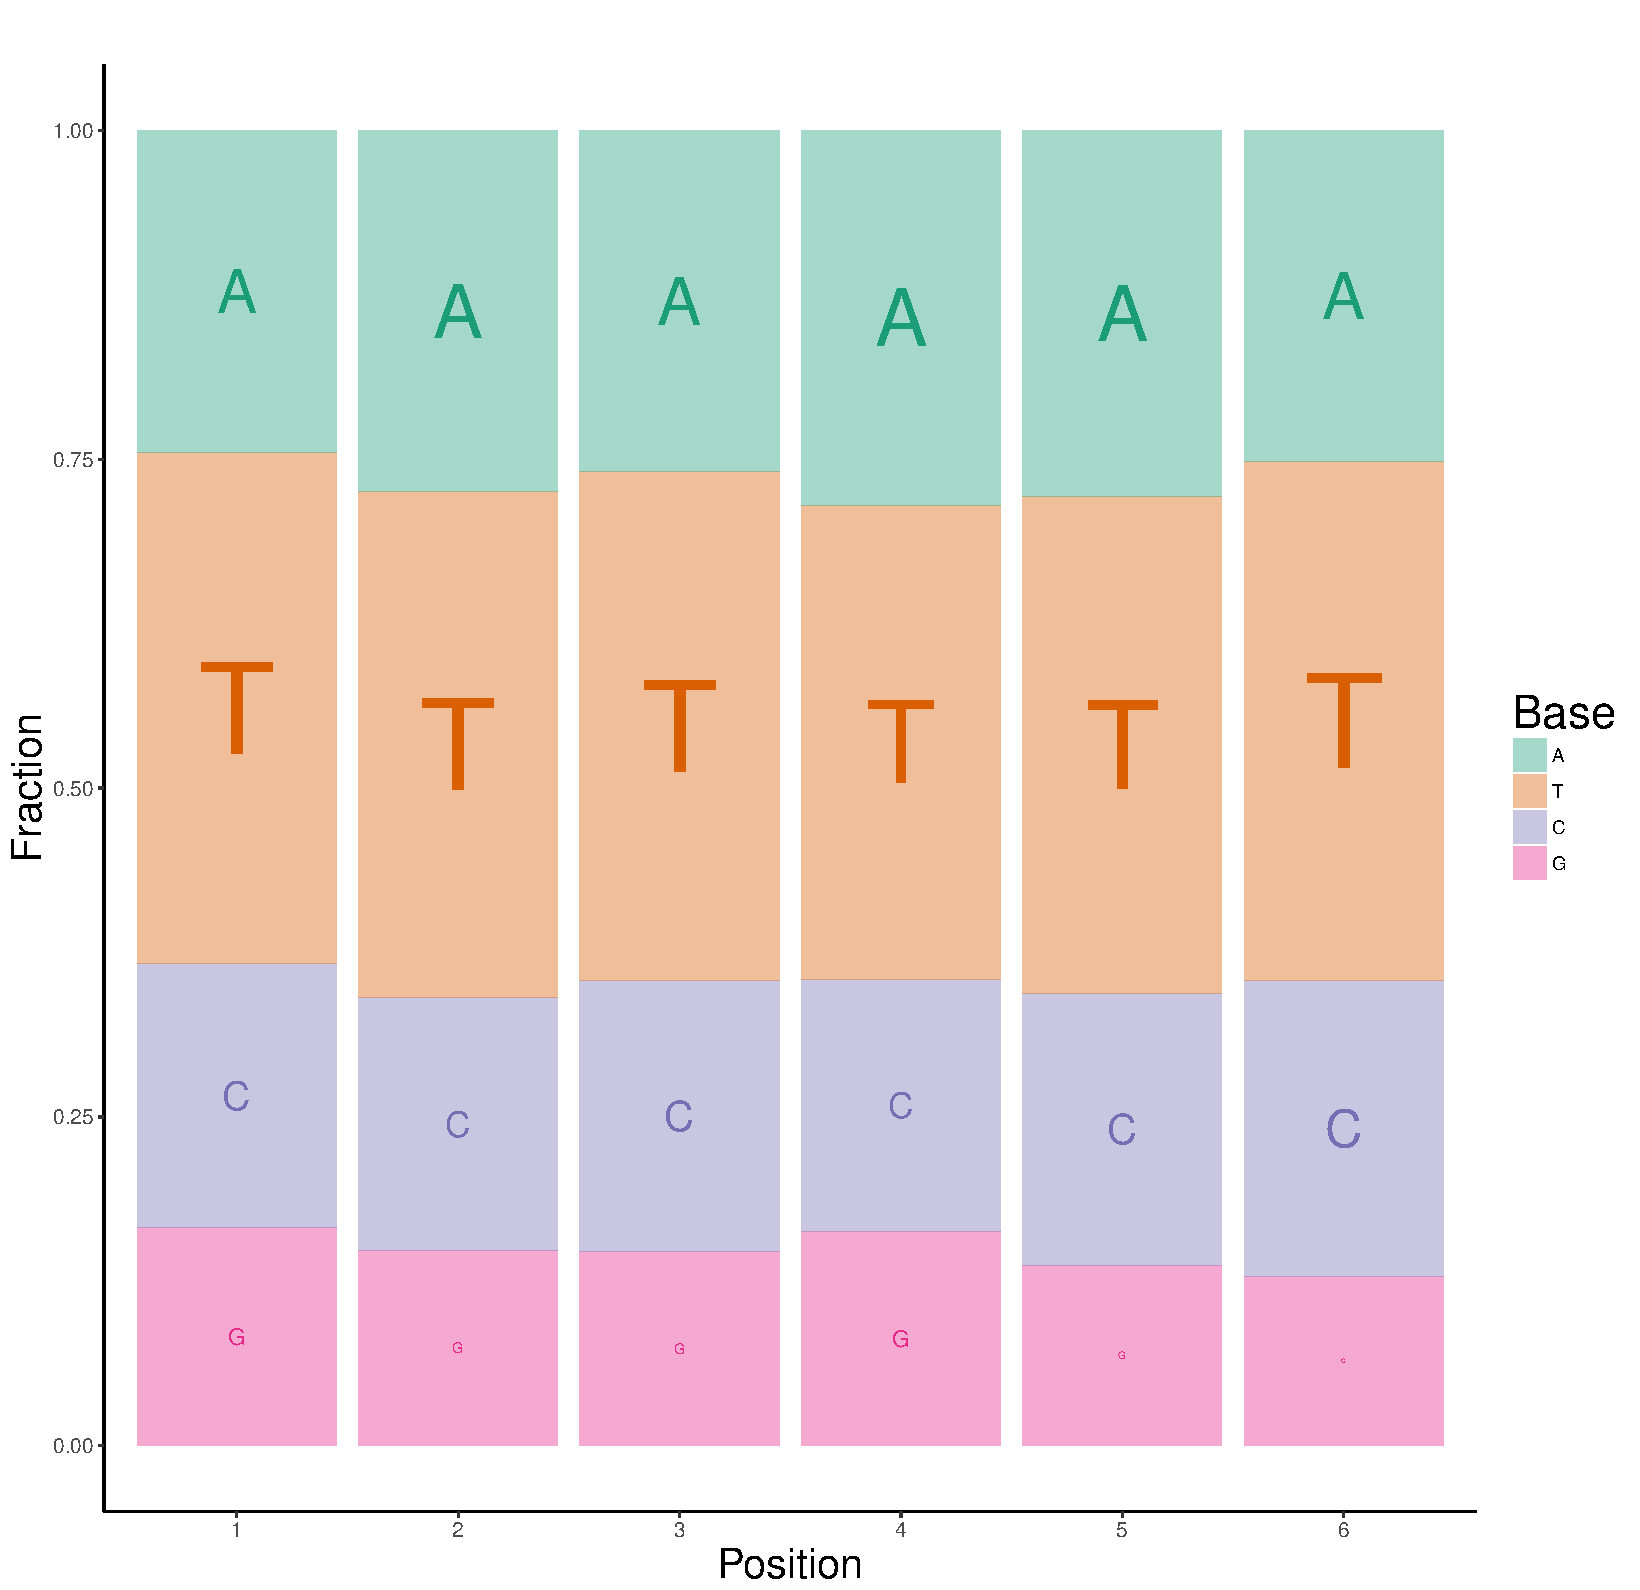
\includegraphics[scale=0.13, trim={0 0 3cm 0}, clip]{primer_usage_ppm_R.pdf}}
      \only<3>{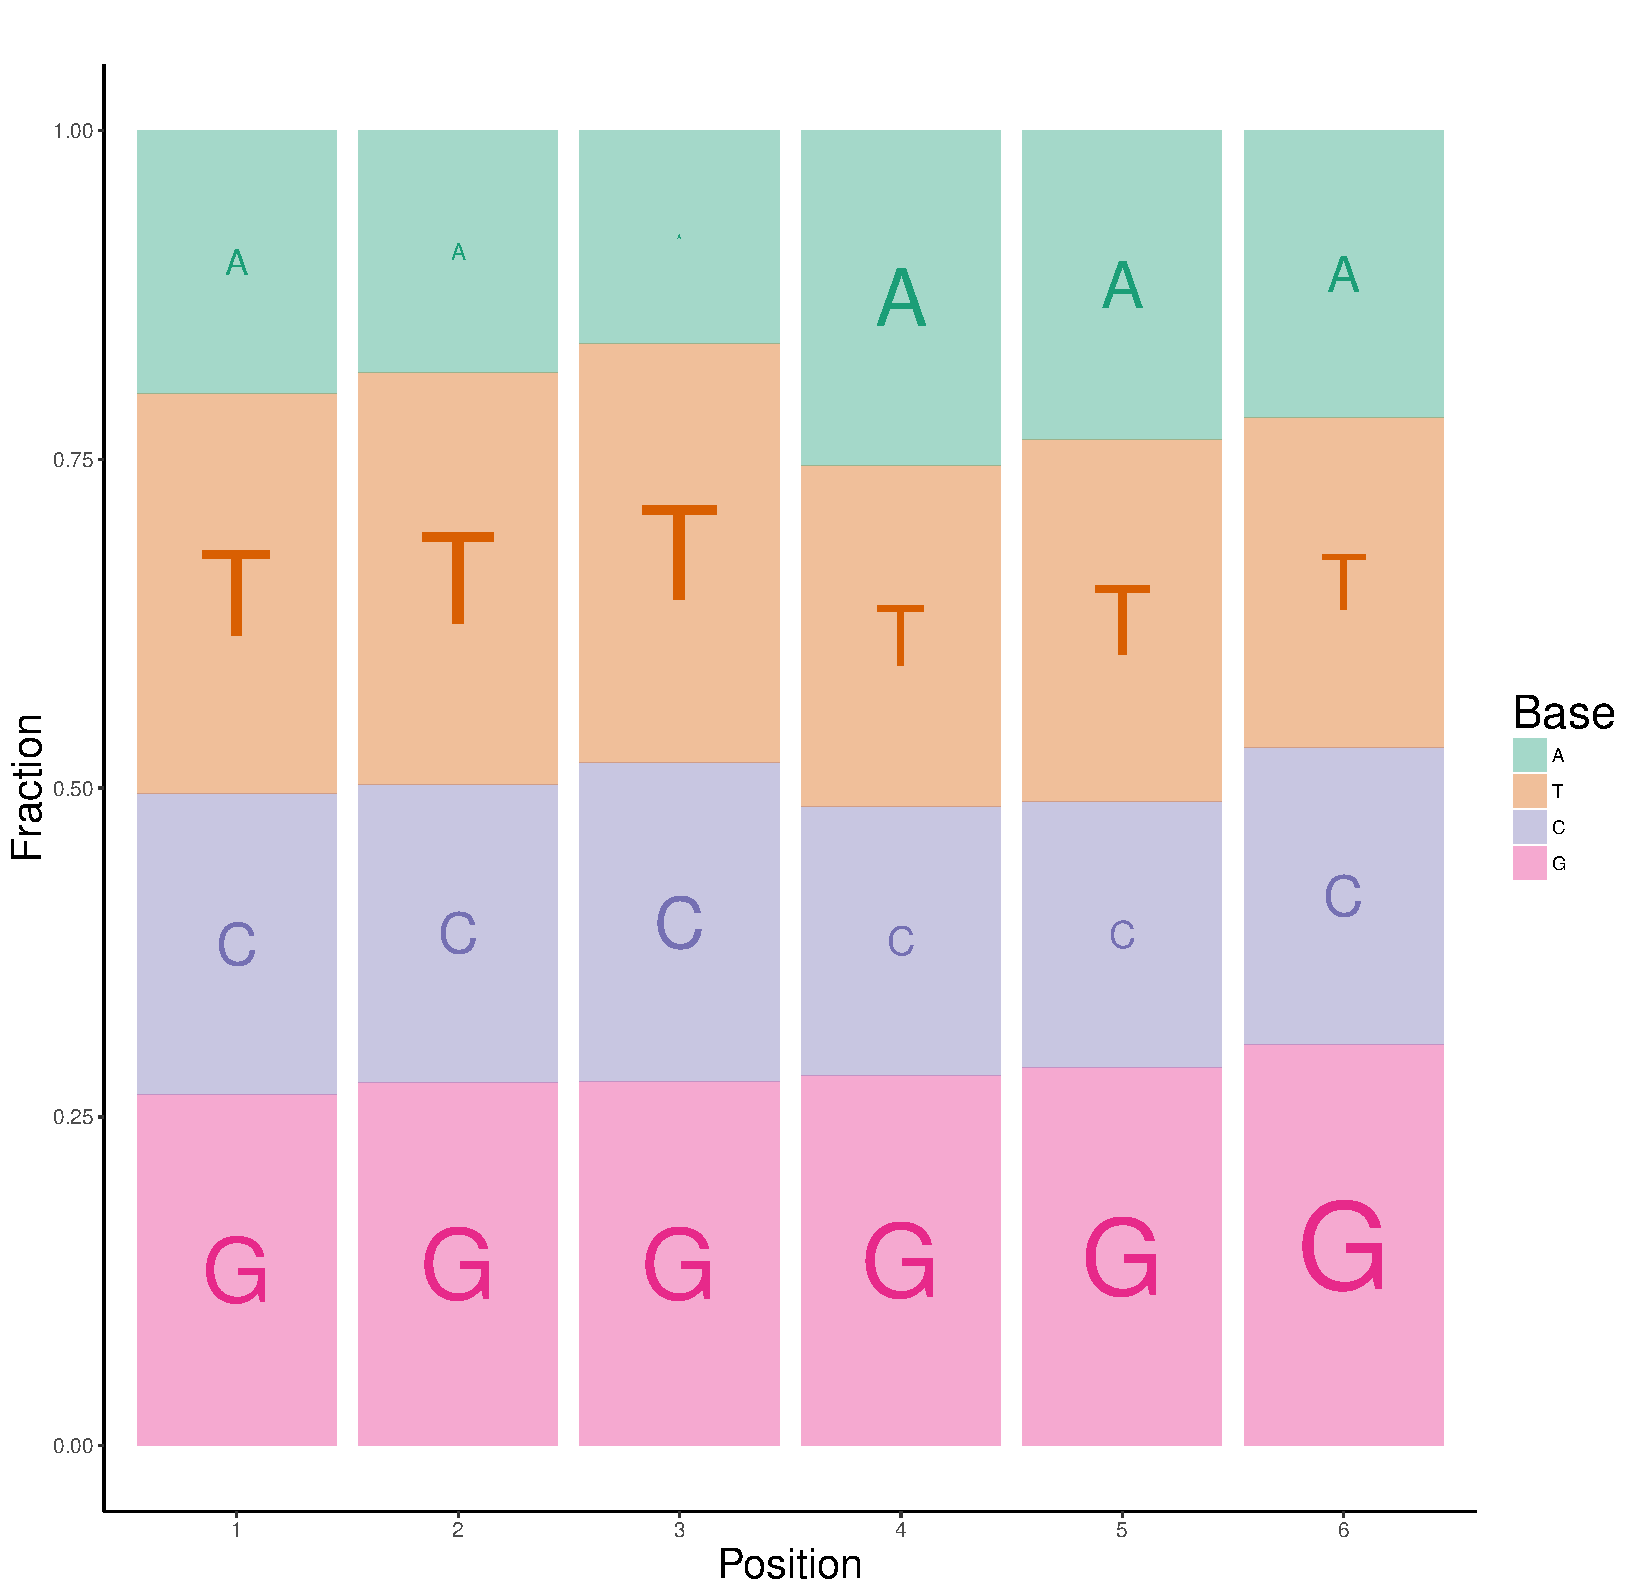
\includegraphics[scale=0.13, trim={0 0 3cm 0}, clip]{template_usage_ppm_R.pdf}}
      \end{figure}
      }
    \end{column}
    \begin{column}{0.3\linewidth}
      \centering{
      T = 45\% T, 5\% G
      \vspace{-0.2cm}
      \begin{figure}
      \only<1>{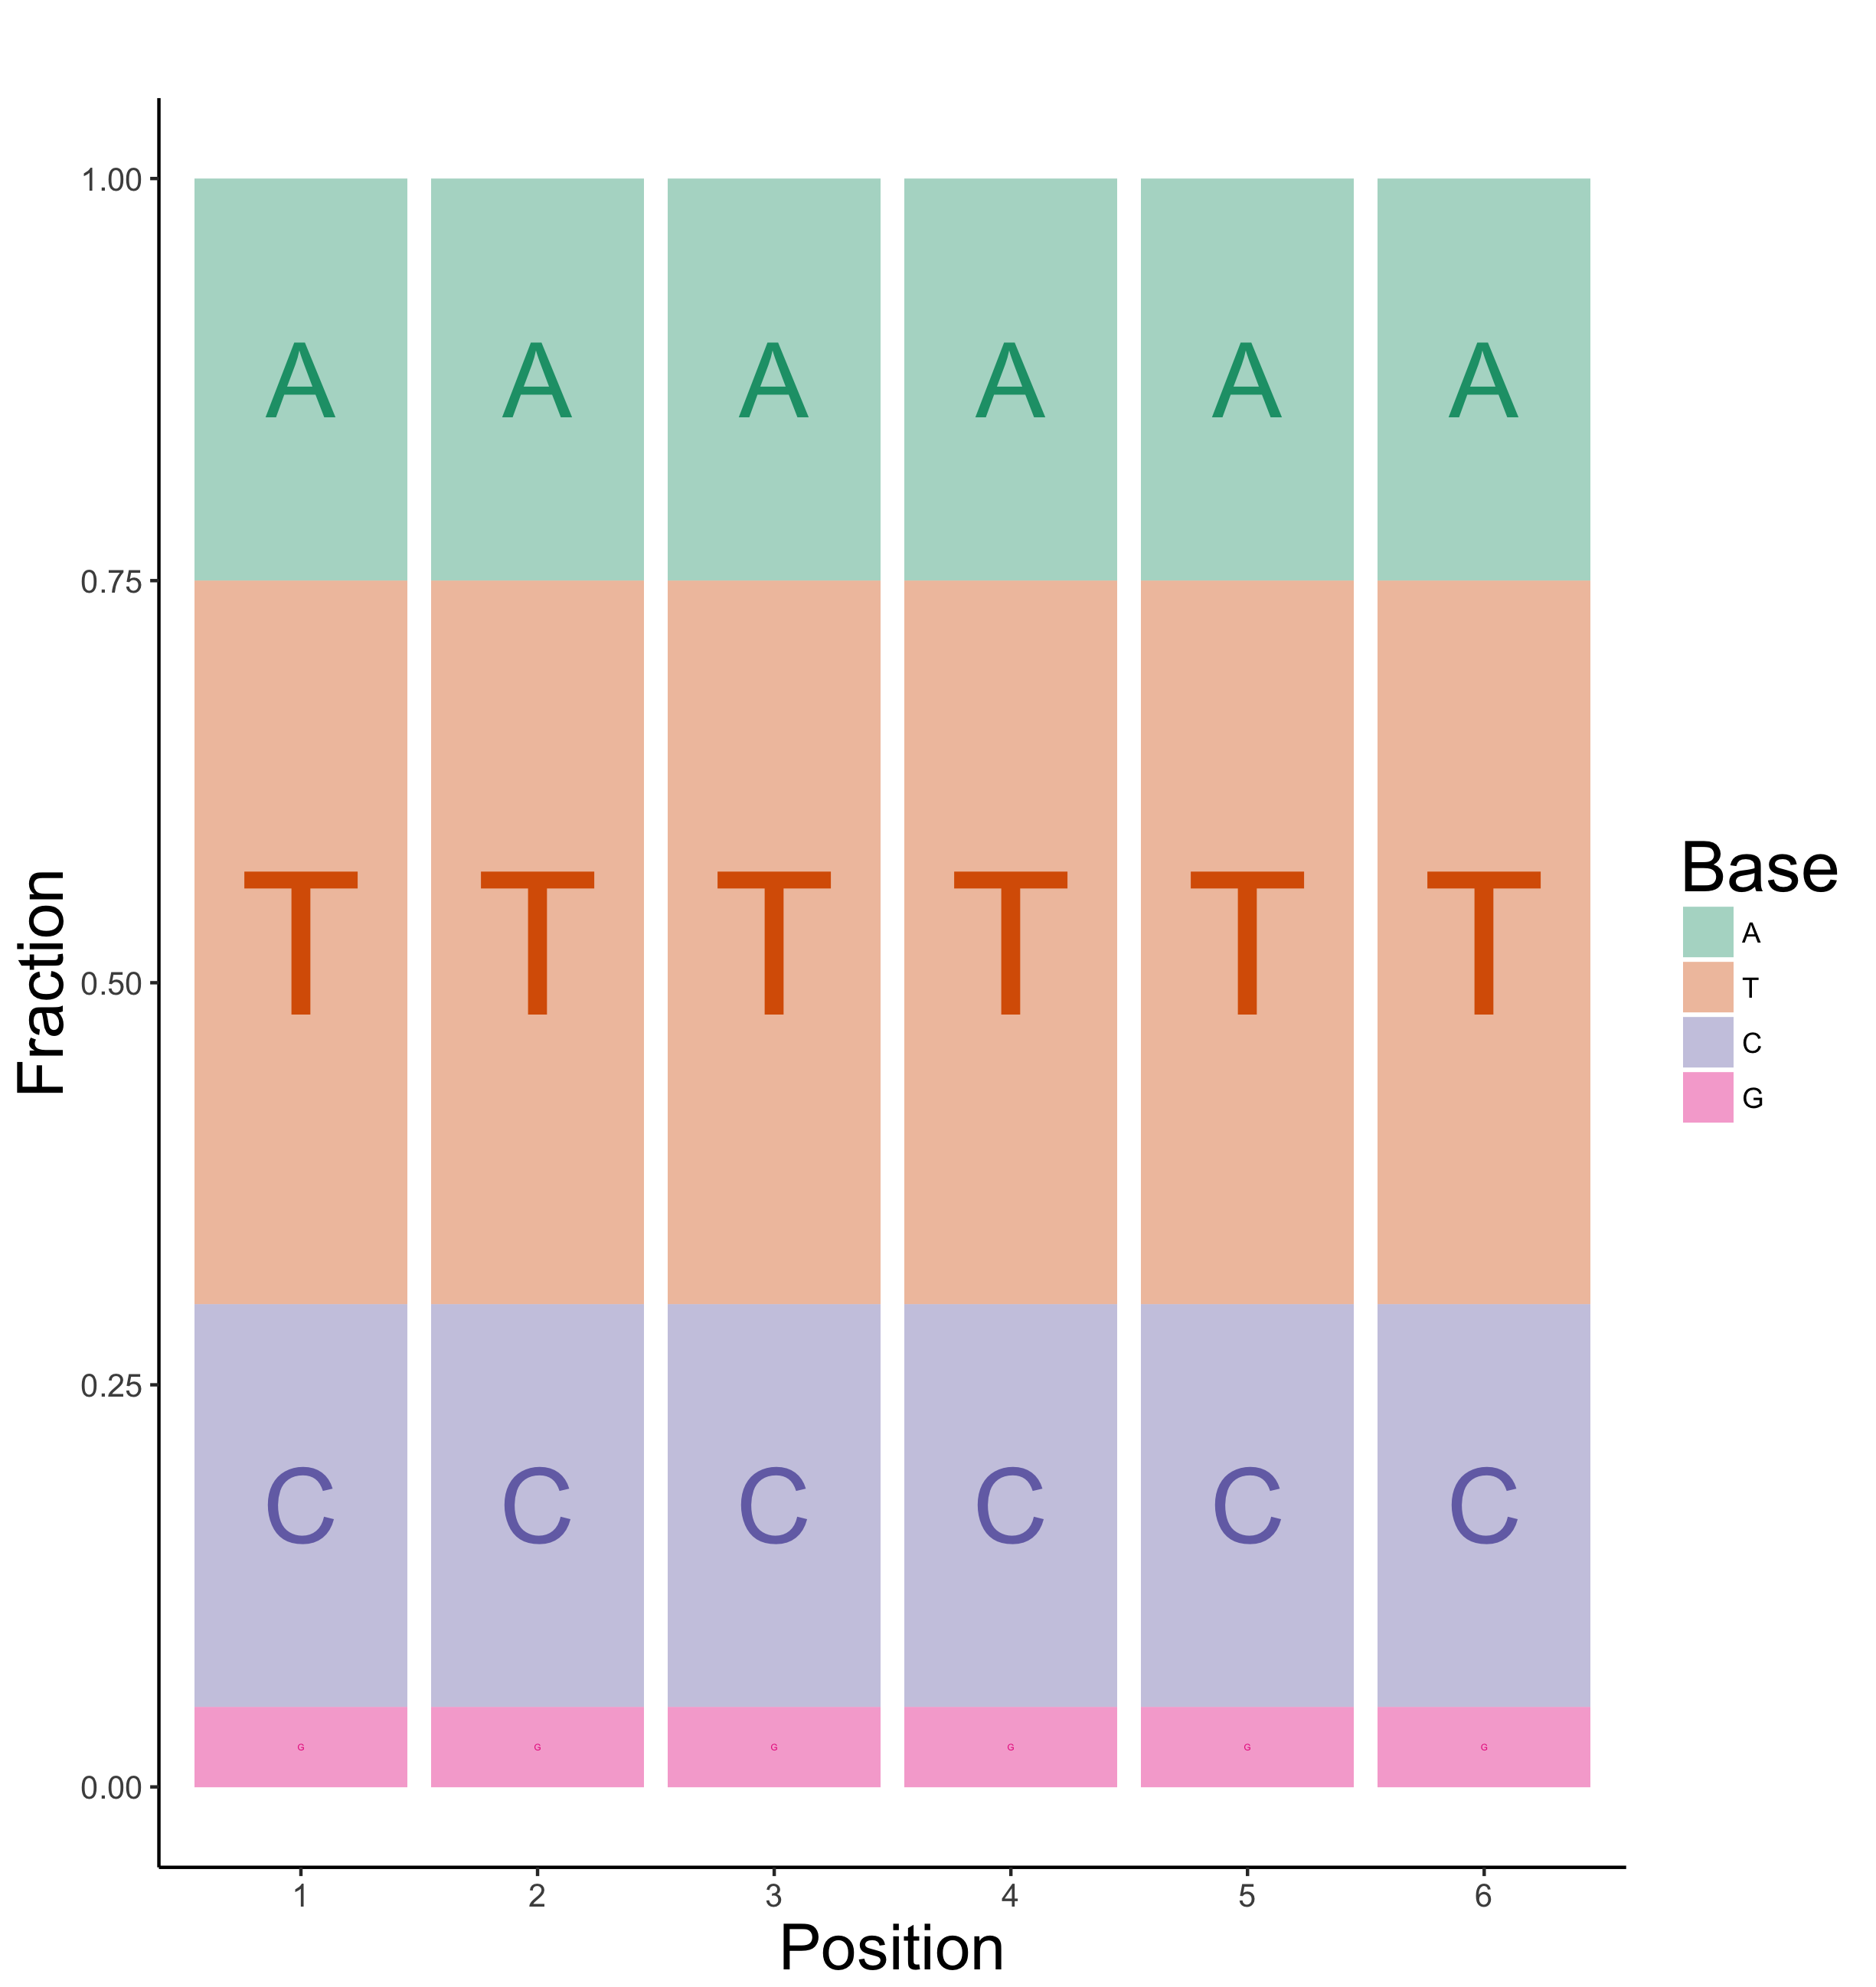
\includegraphics[scale=0.04, trim={0 0 9cm 7cm}, clip]{ppm_T.png}}
      \only<2>{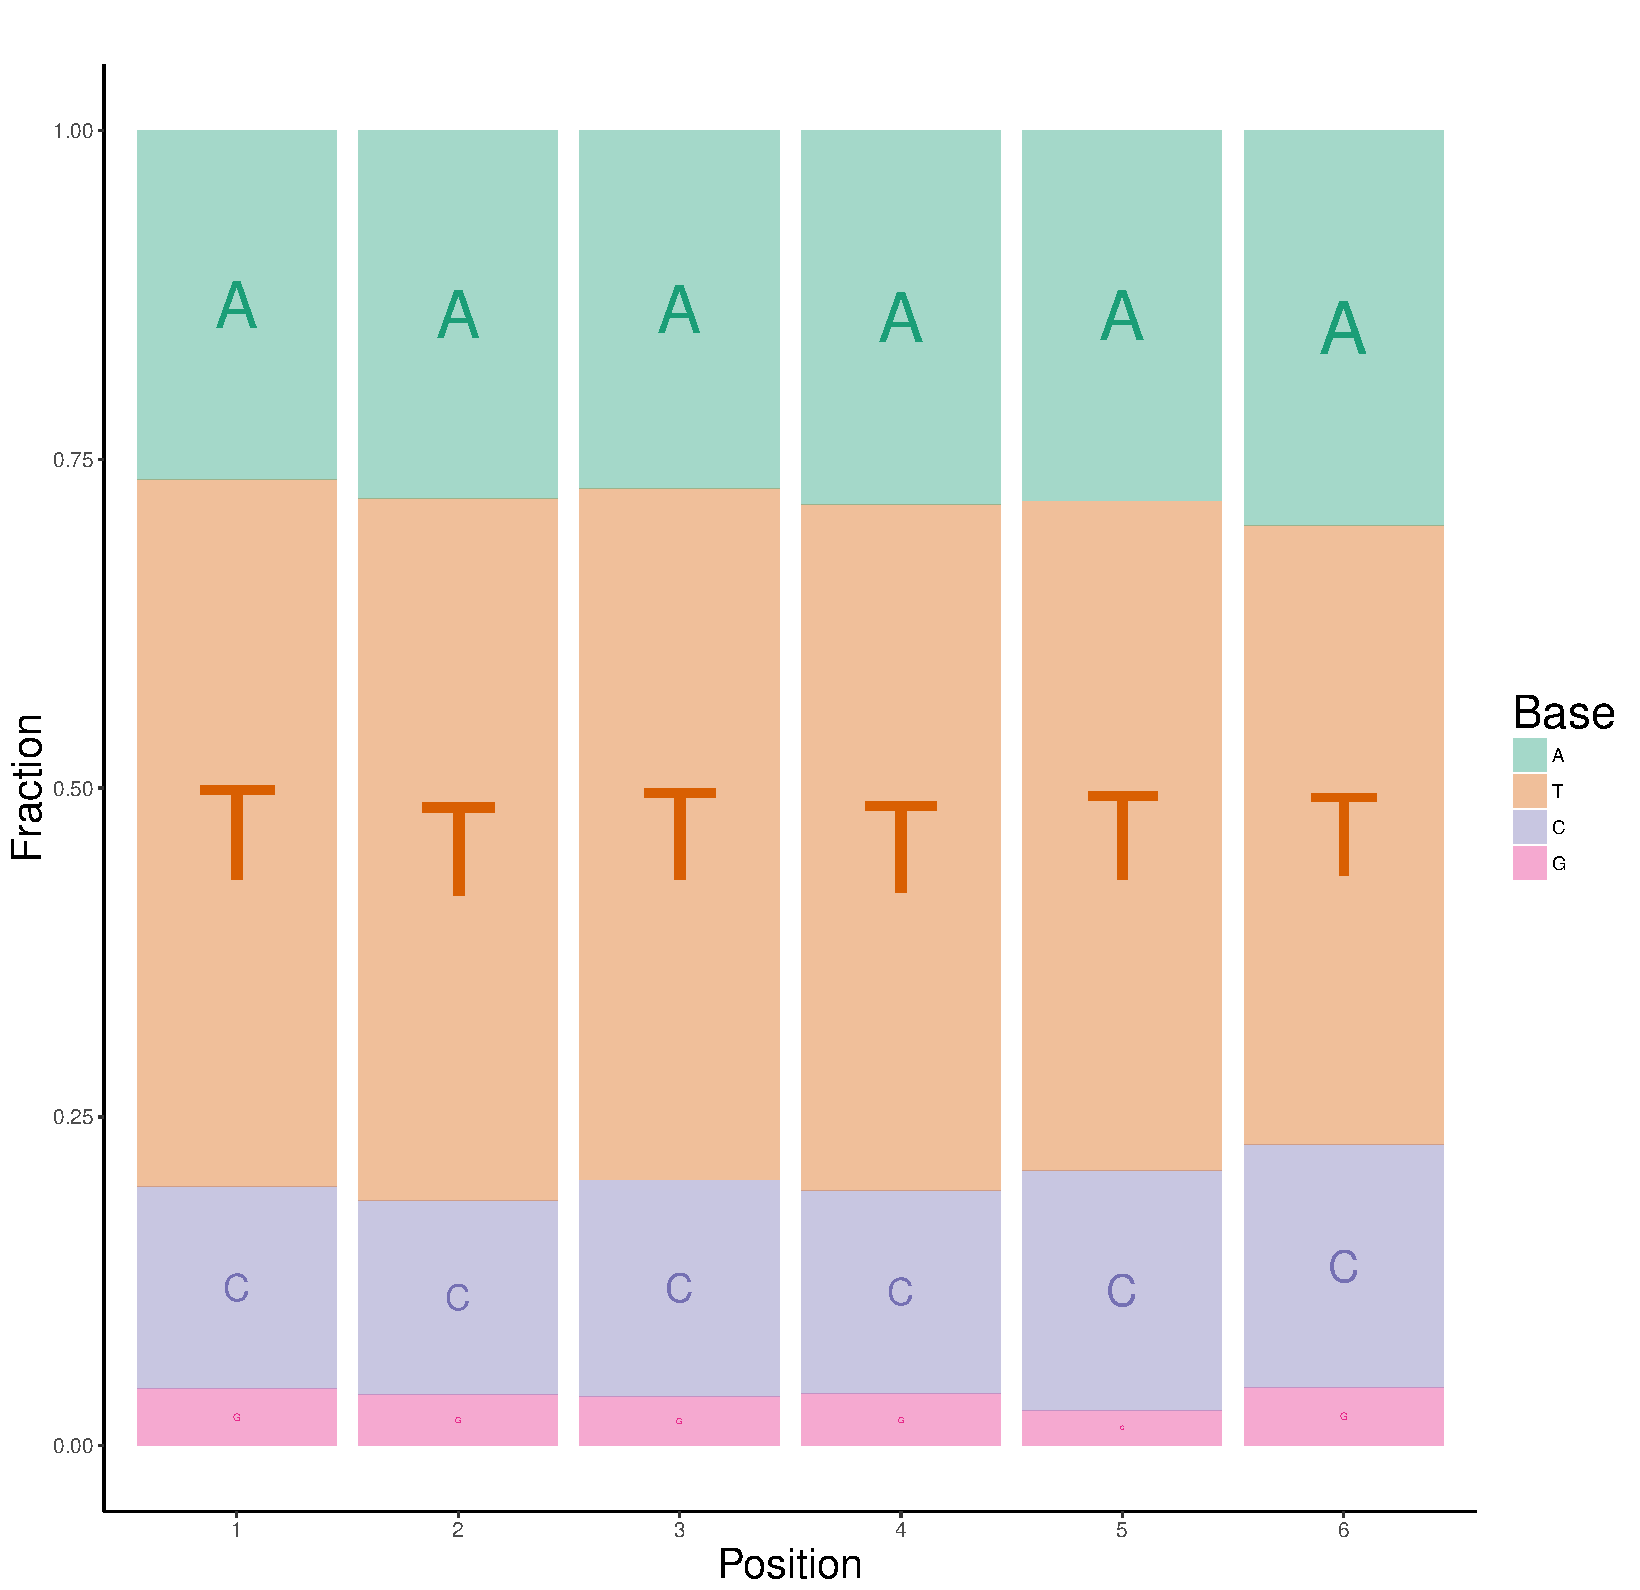
\includegraphics[scale=0.13, trim={0 0 3cm 0}, clip]{primer_usage_ppm_T.pdf}}
      \only<3>{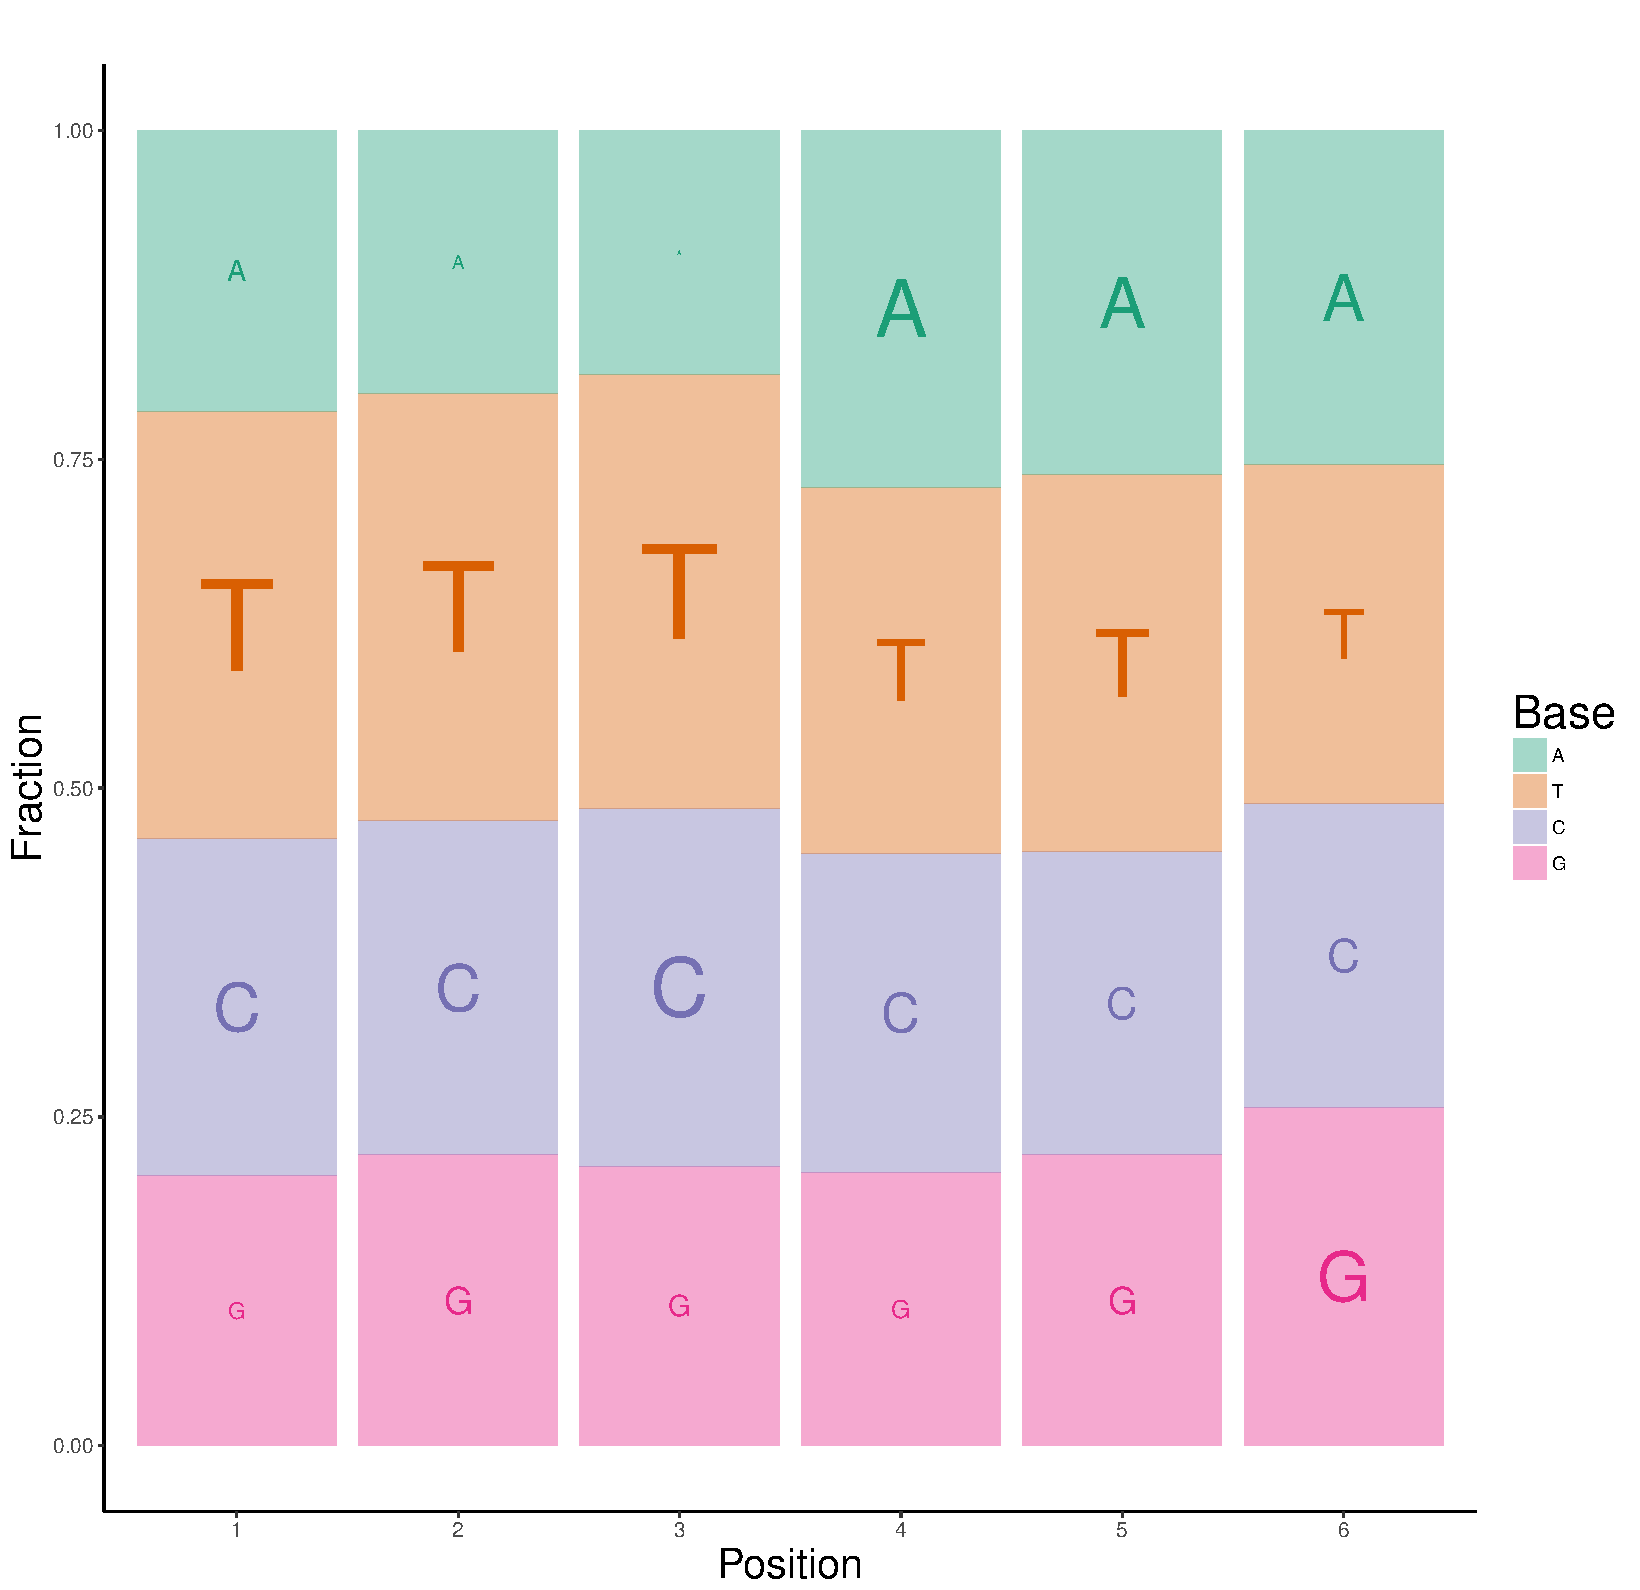
\includegraphics[scale=0.13, trim={0 0 3cm 0}, clip]{template_usage_ppm_T.pdf}}
      \end{figure}
      }
    \end{column}
    \begin{column}{0.3\linewidth}
      \centering{
      G = 45\% G, 5\% T
      \vspace{-0.2cm}
      \begin{figure}
      \only<1>{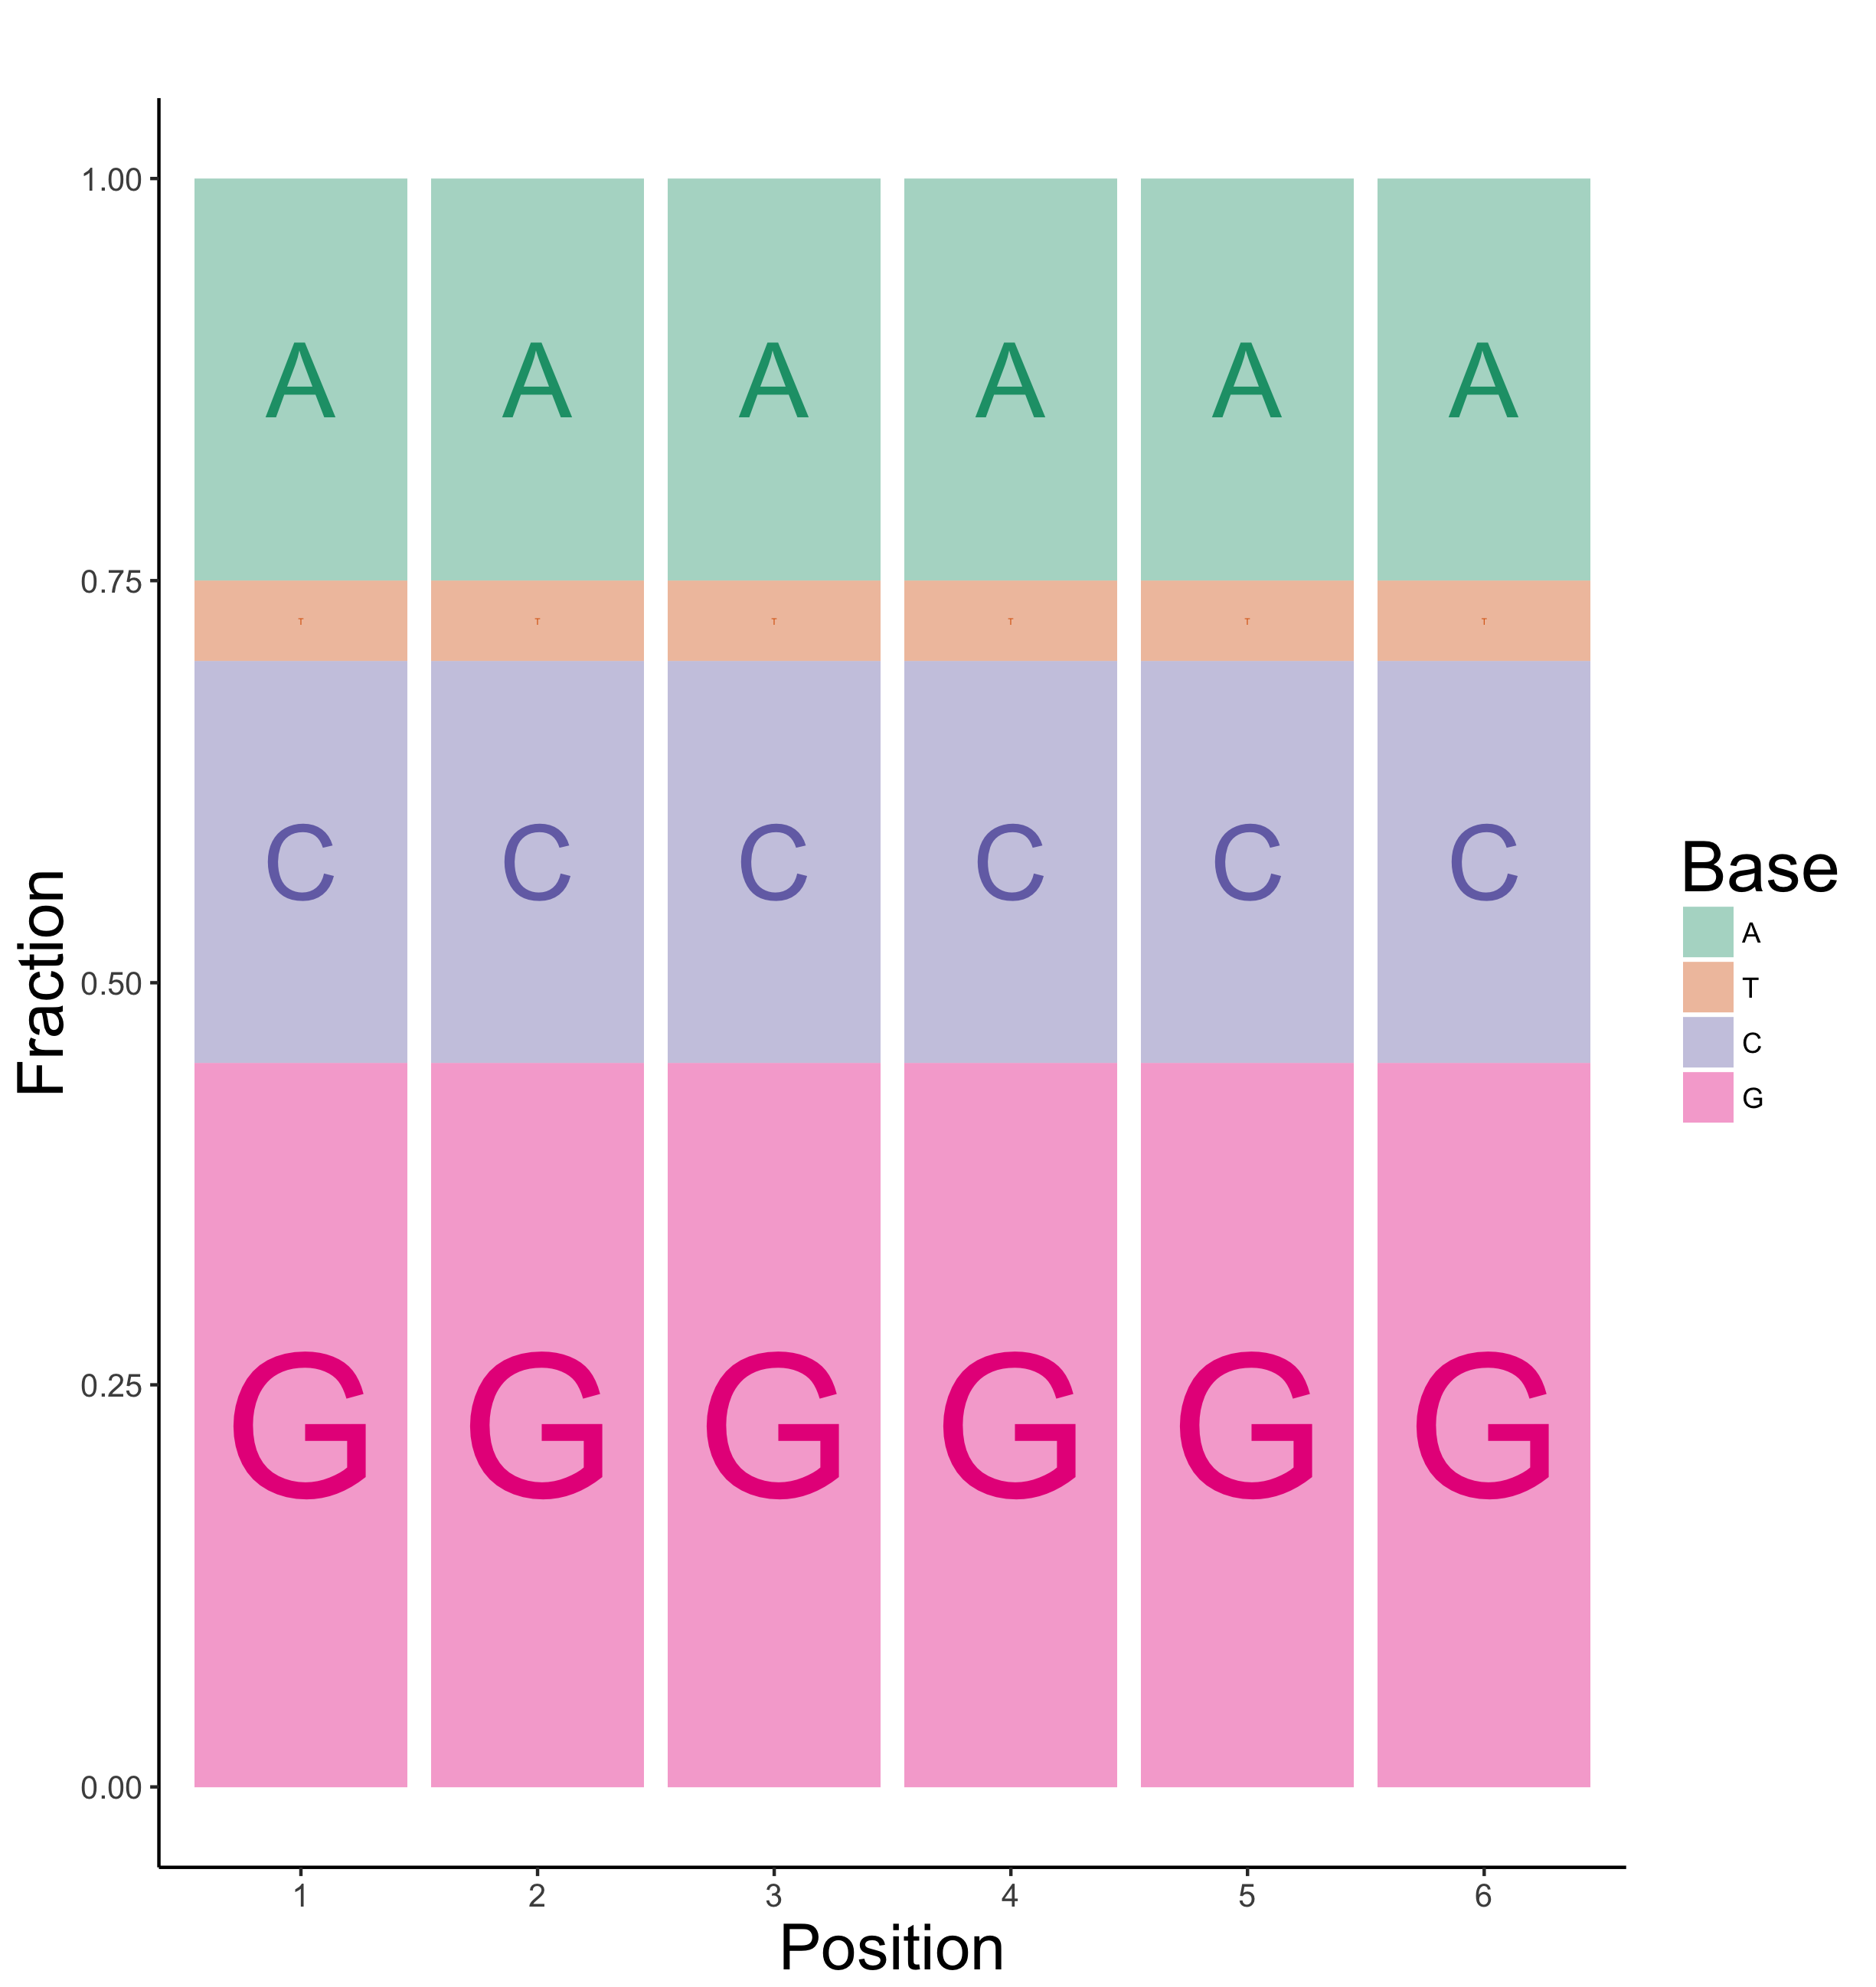
\includegraphics[scale=0.04, trim={0 0 9cm 7cm}, clip]{ppm_G.png}}
      \only<2>{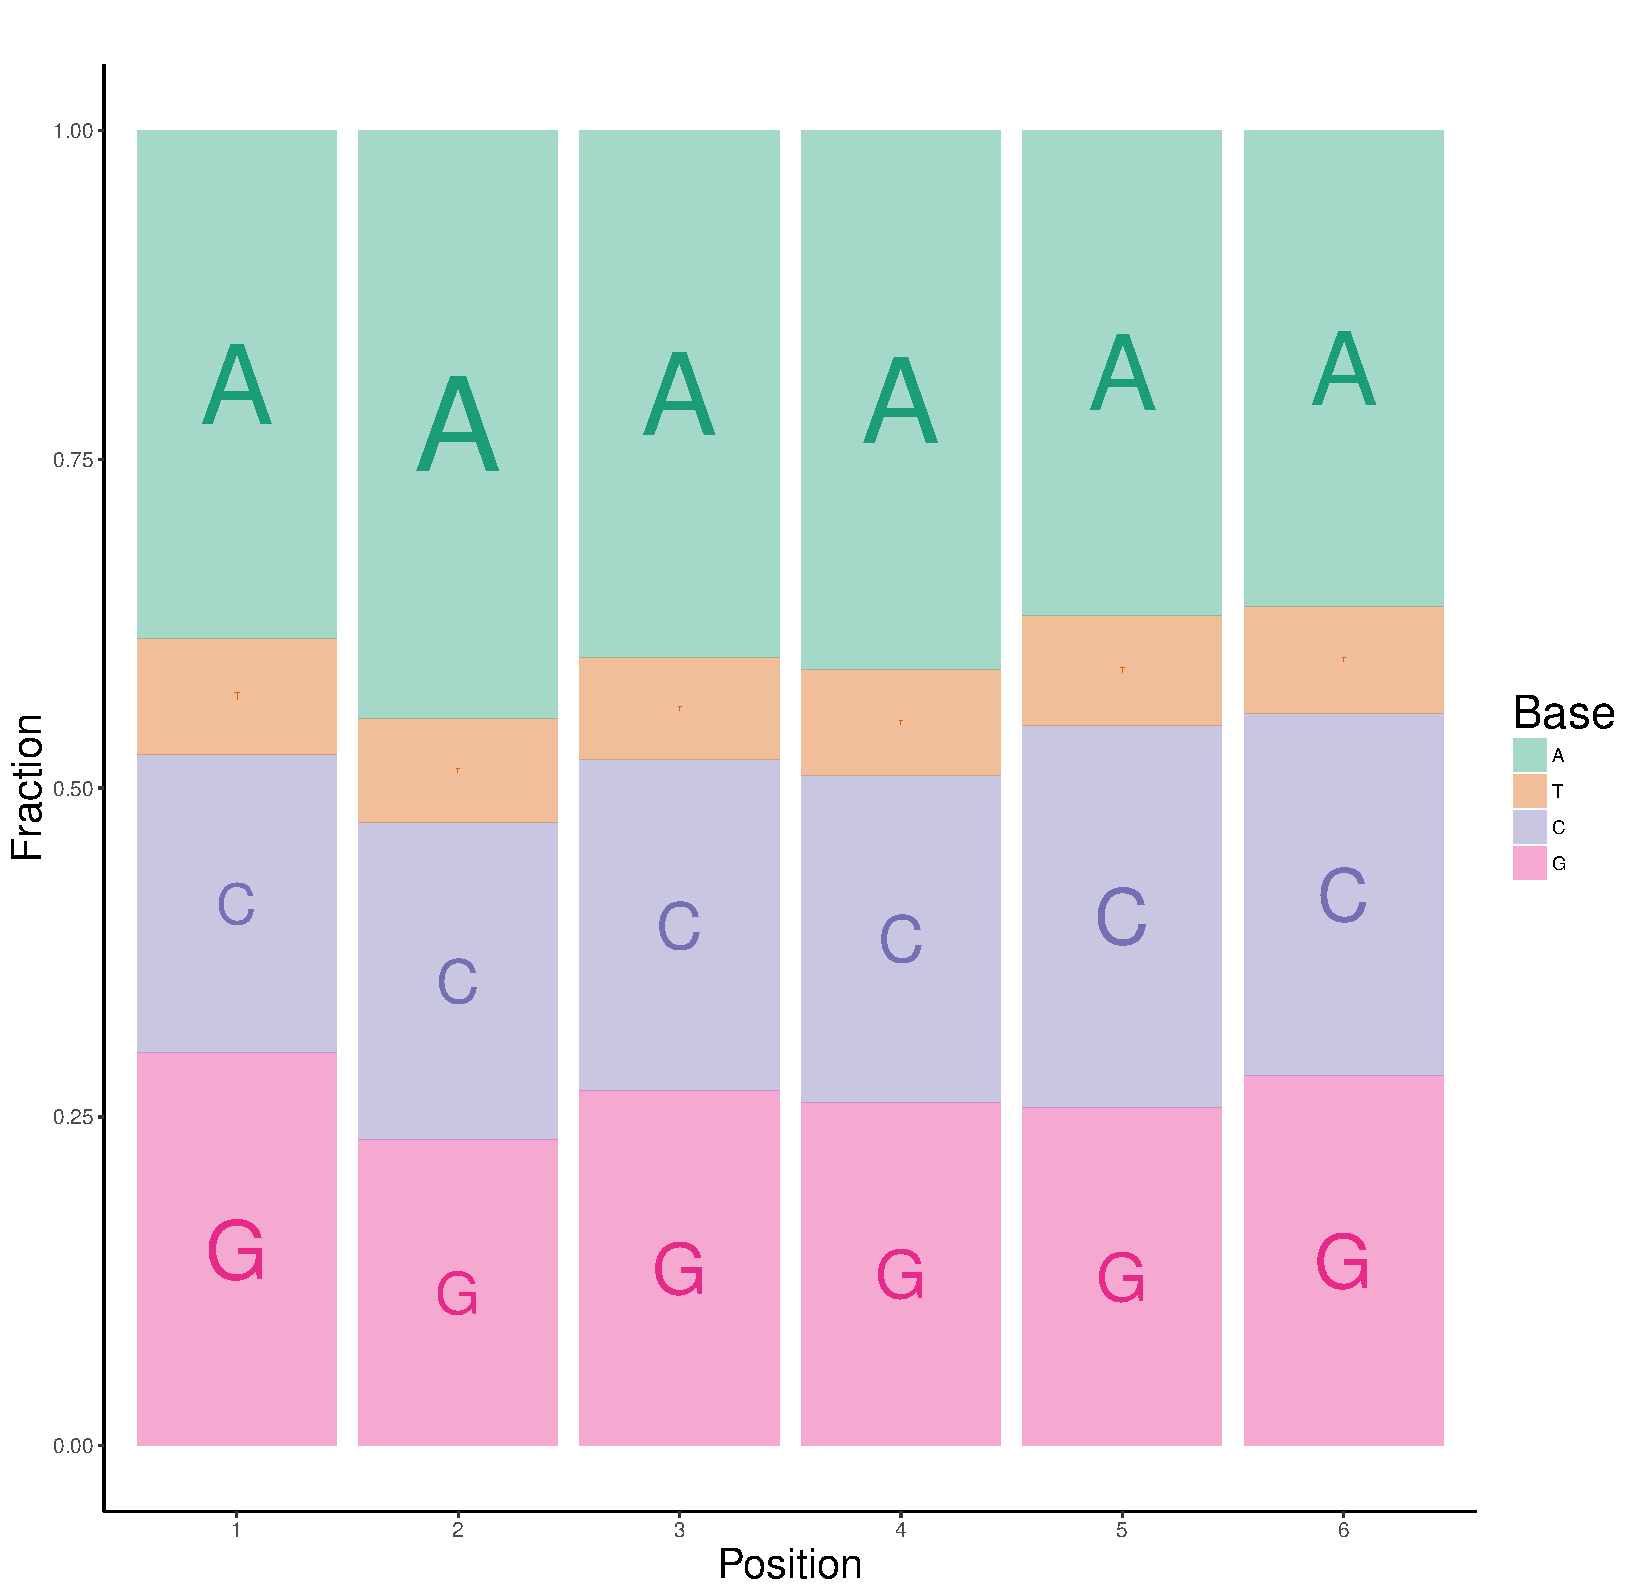
\includegraphics[scale=0.13, trim={0 0 3cm 0}, clip]{primer_usage_ppm_G.pdf}}
      \only<3>{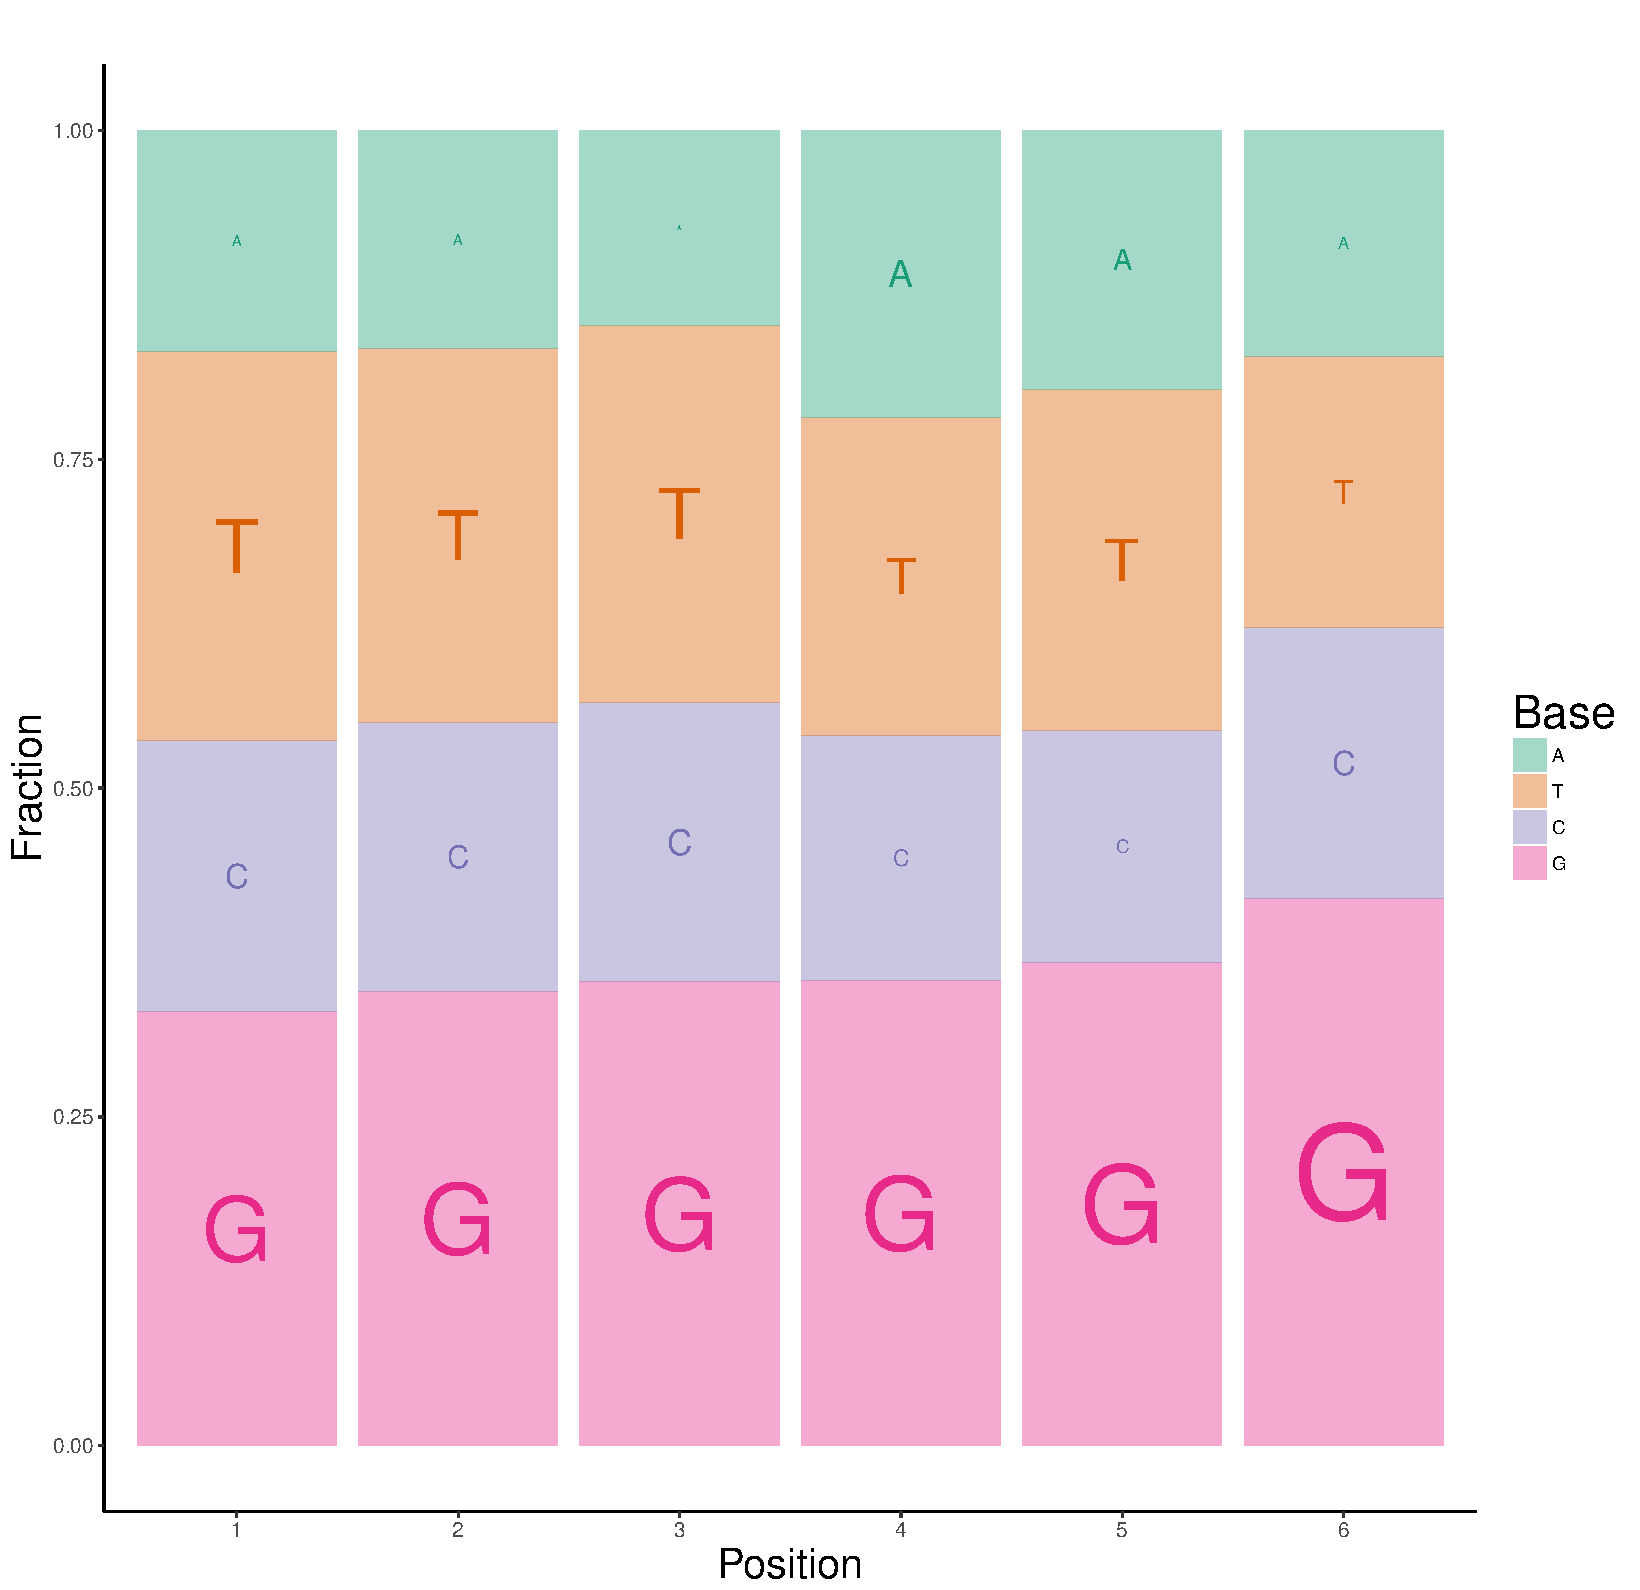
\includegraphics[scale=0.13, trim={0 0 3cm 0}, clip]{template_usage_ppm_G.pdf}}
      \end{figure}
      }
    \end{column}
  \end{columns}
  % }
\end{frame}

\begin{frame}{Altered primer batch: coverage bias}
  \begin{figure}
    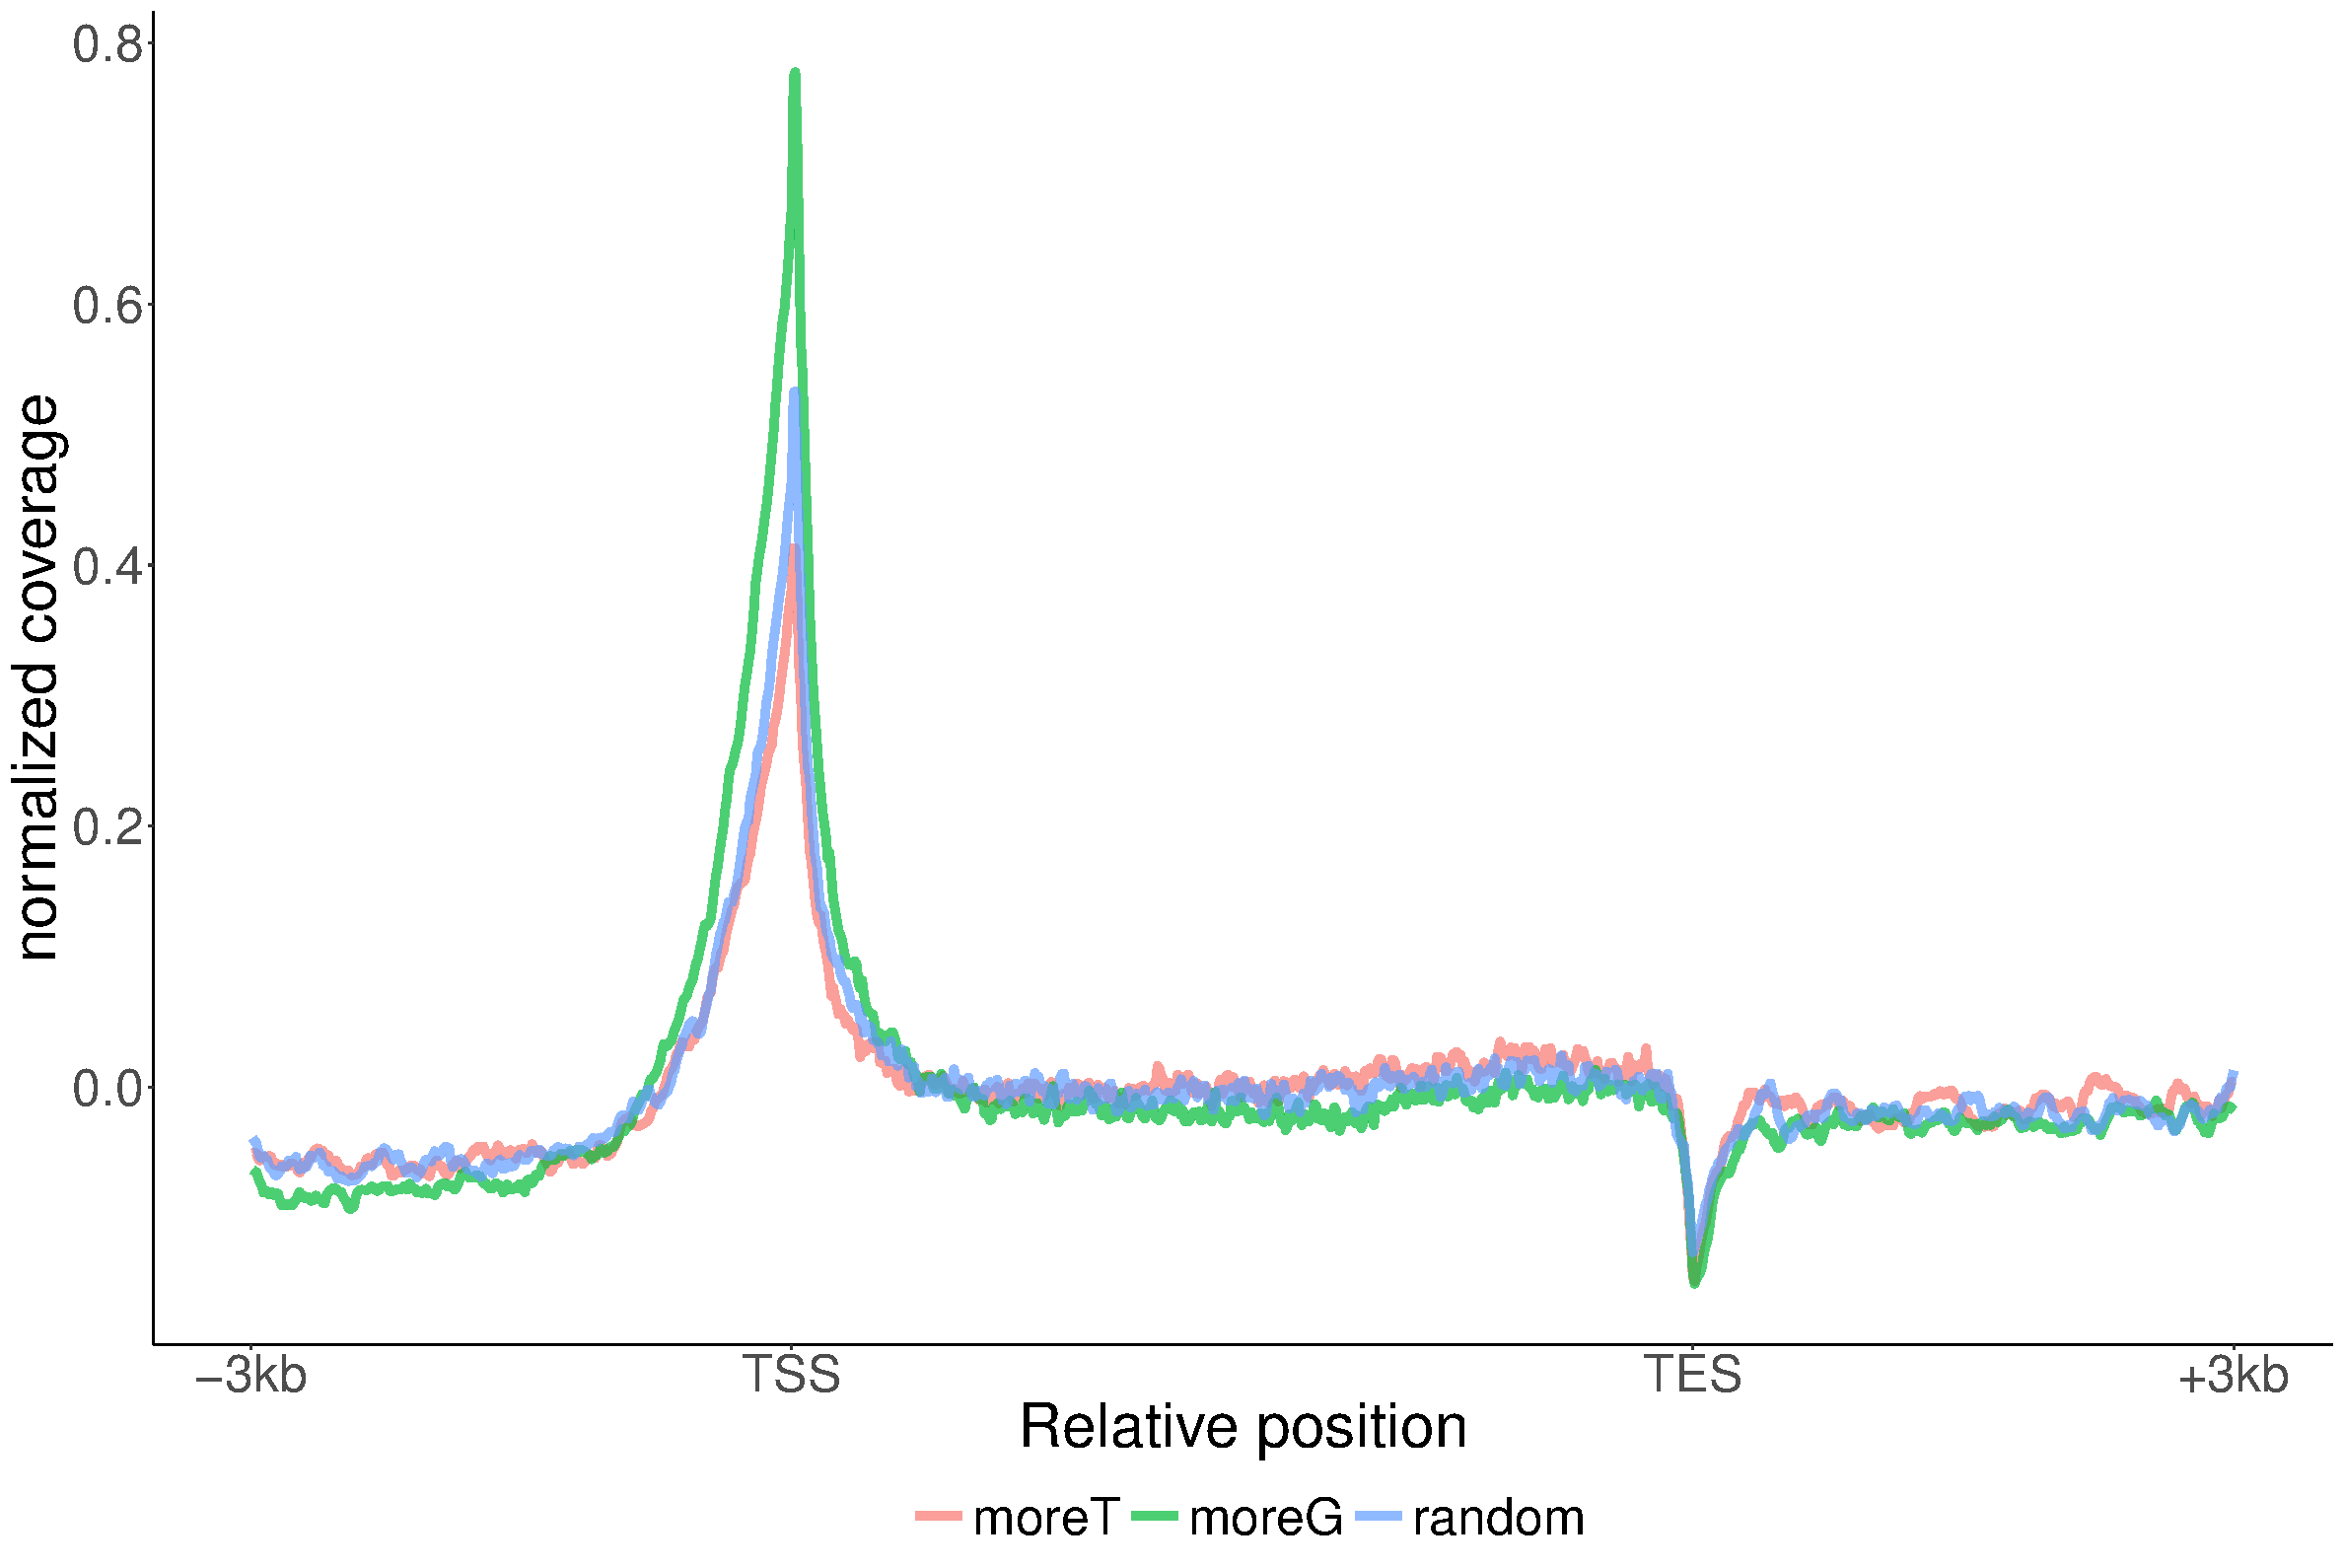
\includegraphics[scale=0.25]{bias_profiles_D2.pdf}
  \end{figure}
\end{frame}

\begin{frame}{}

\end{frame}


% \begin{frame}{Validating $\Delta$F: consistency between experiments}
%   \vspace{-0.2cm}
%   \begin{figure}
%       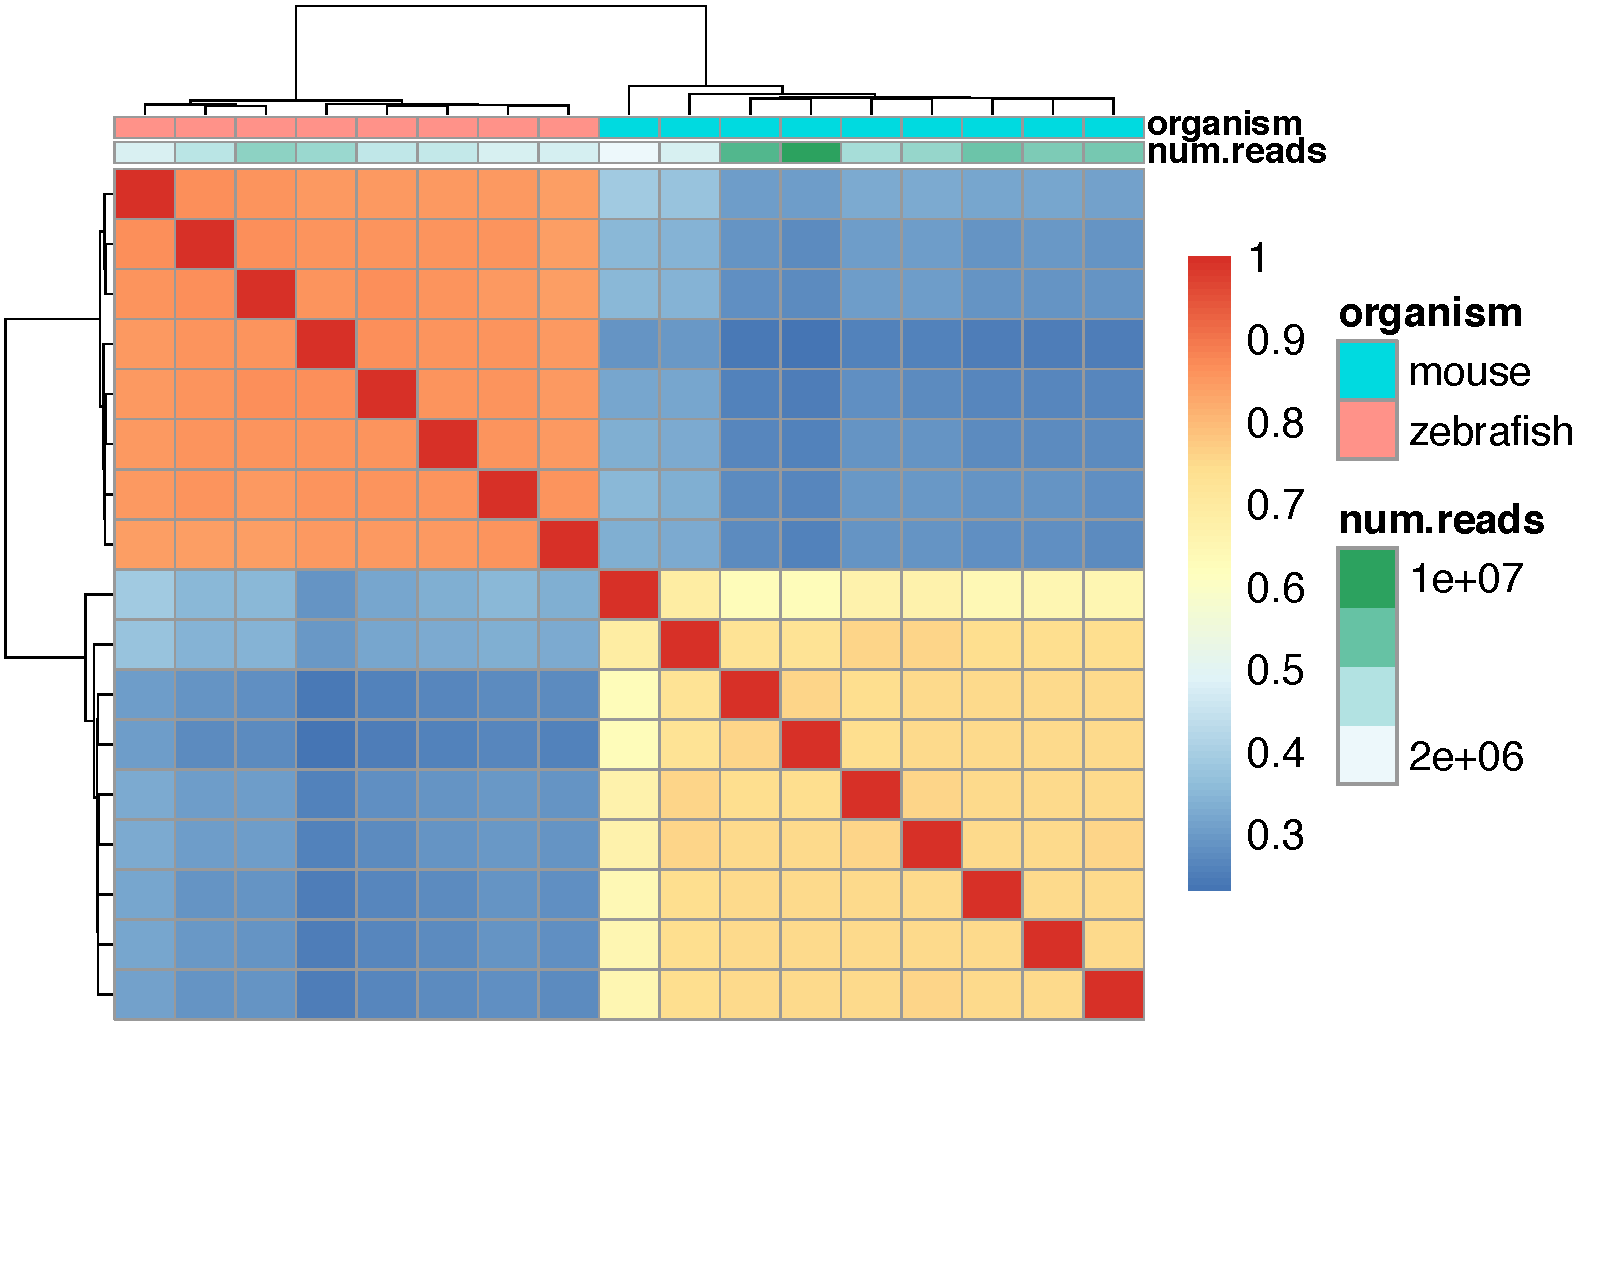
\includegraphics[scale=0.35]{BScorrelation_deltaG_R1.pdf}
%   \end{figure}
% \end{frame}
%
% \begin{frame}{Validating $\Delta$F: consistency with tabulated free-binding energy values}
%   \vspace{-0.3cm}
%       \centering{Hexamers with no C $\longrightarrow \Delta F \equiv \Delta G$}
%       \begin{figure}
%           \centering
%           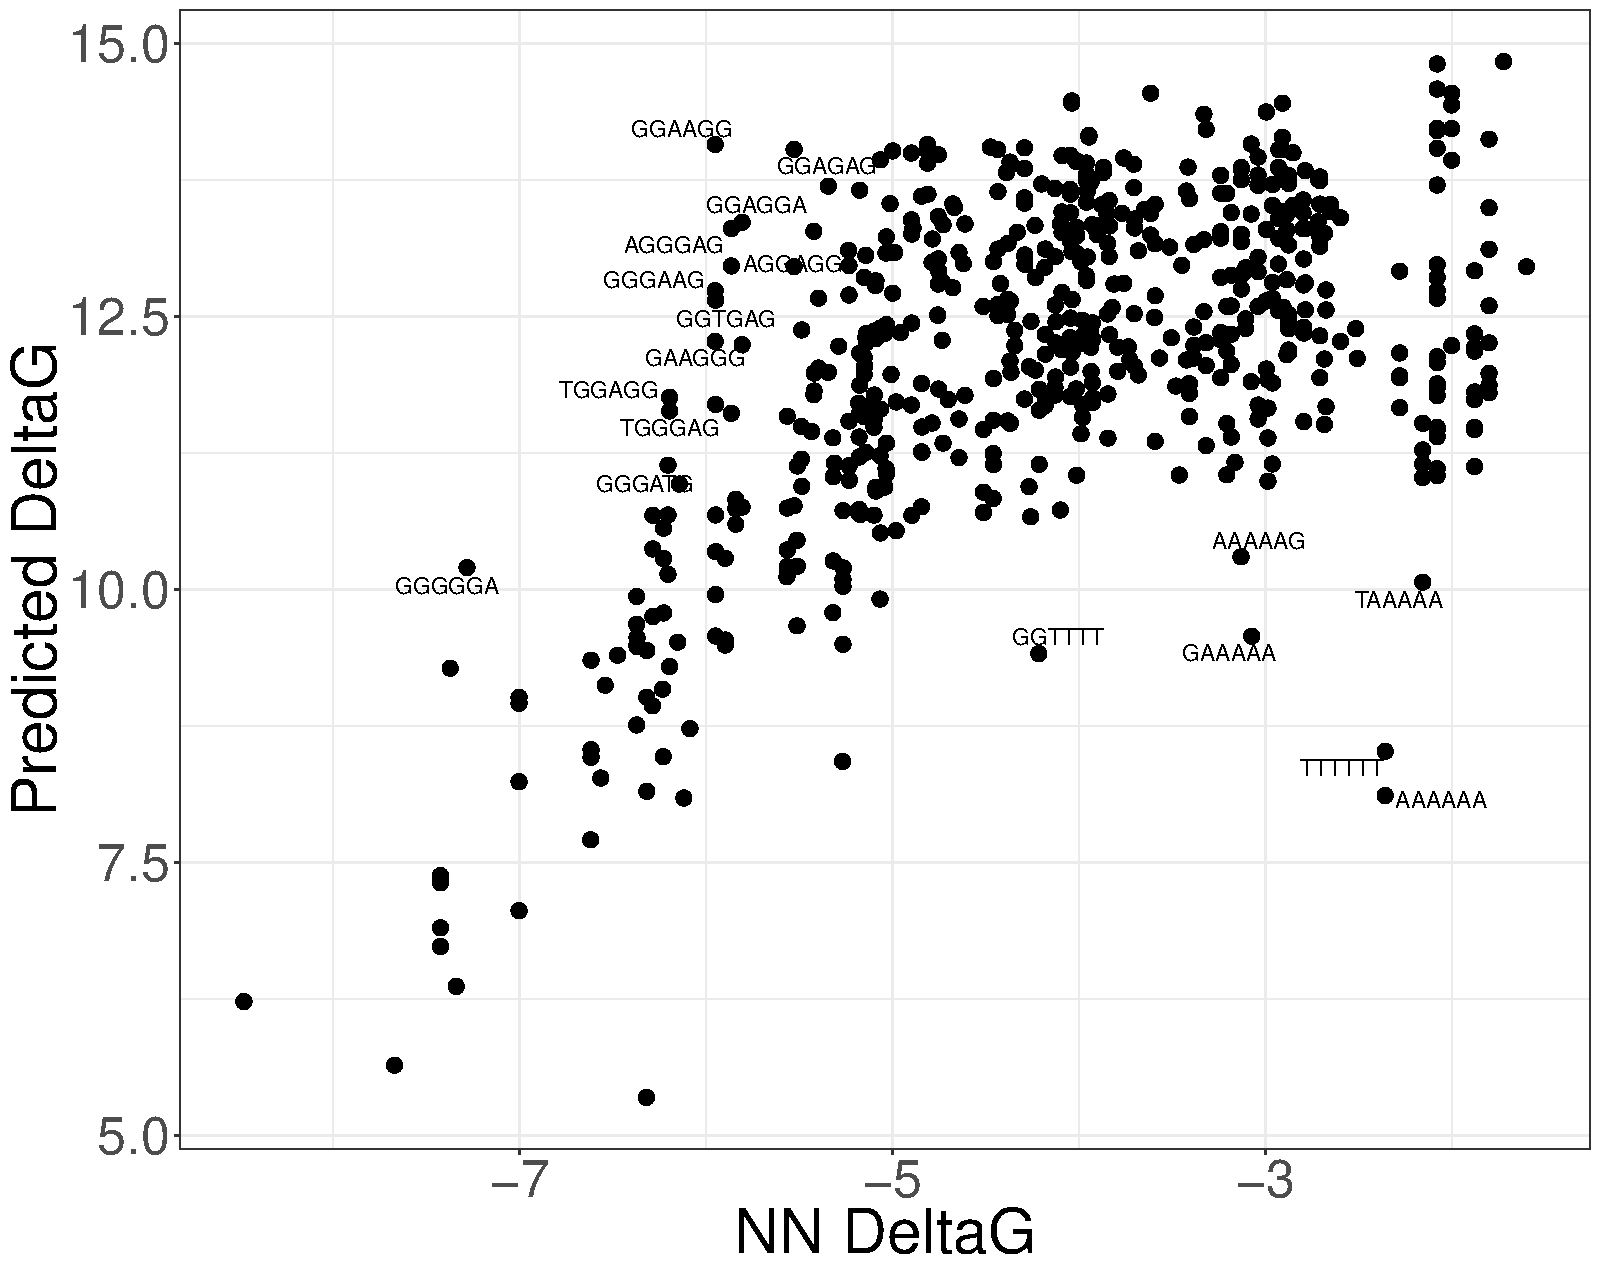
\includegraphics[scale=0.27]{predBsVSnnmodel_noC_strandSpecific.pdf}
%       \end{figure}
%   \onslide<2>{
%   \begin{center}
%     \alert{Ongoing: generating data on non-converted samples for \\
%     validation of $\Delta G$ prediction}
%   \end{center}
%   }
% \end{frame}
%
% \begin{frame}{Predicted coverage from $\Delta$F}
%   \begin{figure}
%       \centering
%       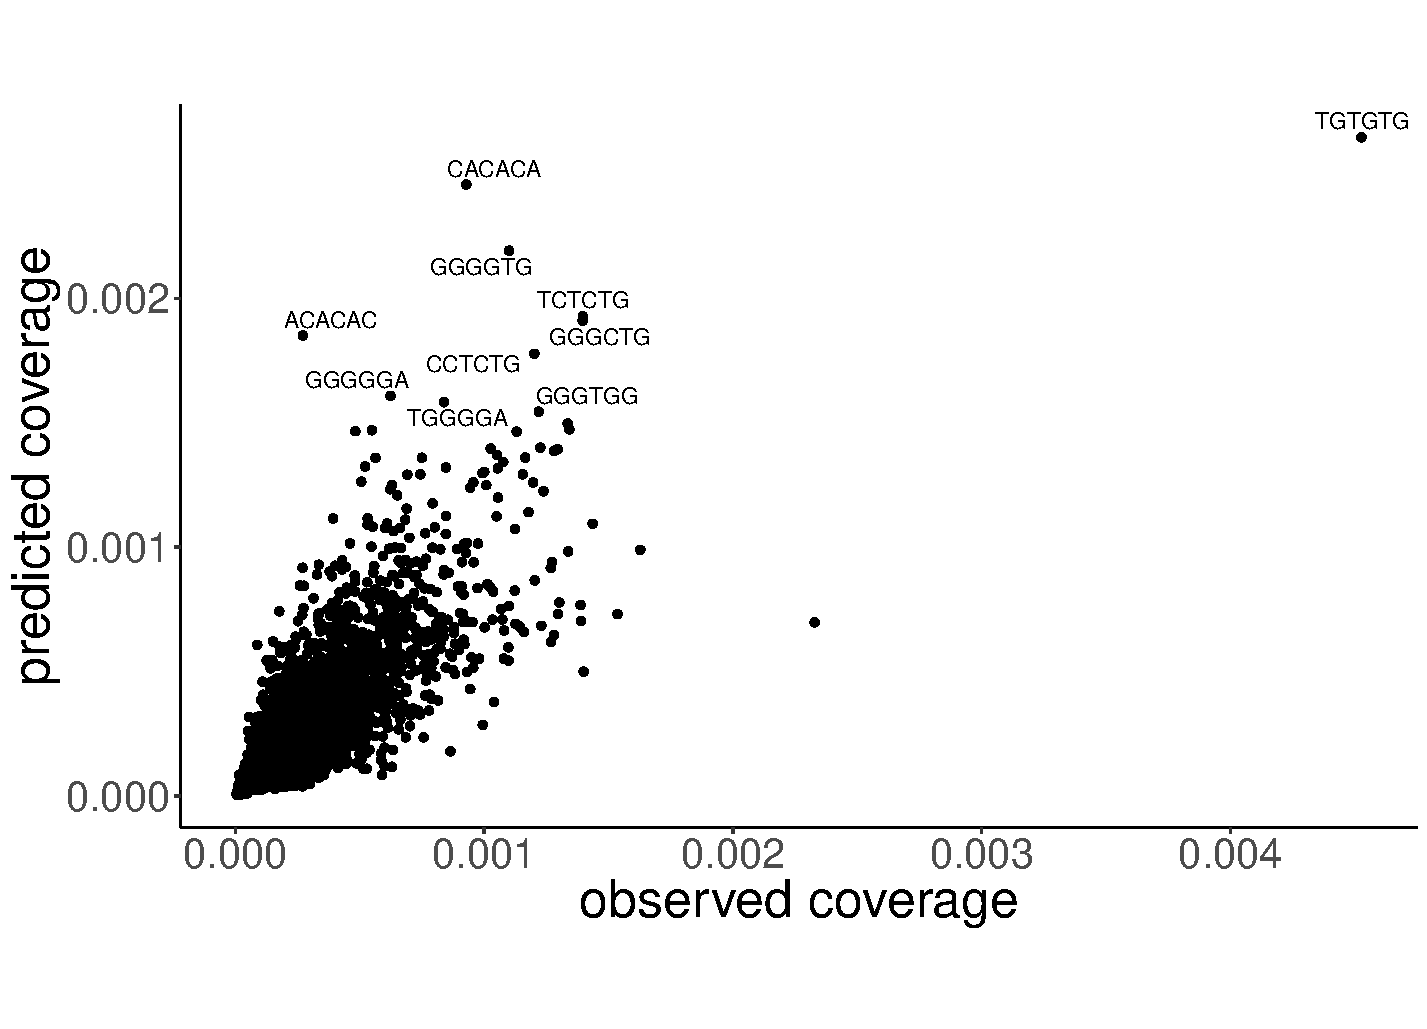
\includegraphics[scale=0.35]{predictedCov_VAN1815_L2_pooledVAN1667.pdf}
%       % \caption{Caption}
%       % % \label{fig:my_label}
%   \end{figure}
%   \onslide<2>{
%   \begin{center}
%     \alert{Does binding explain the spatial genome-wide distribution of coverage?}
%   \end{center}
%   }
% \end{frame}
%
% \begin{frame}{Positional information from binding probability}
%   \Wider{
%   \vspace{-0.4cm}
%   % \centering{Coverage density: $D_j = \frac{C_j}{T_j}$}
%   \begin{figure}
%     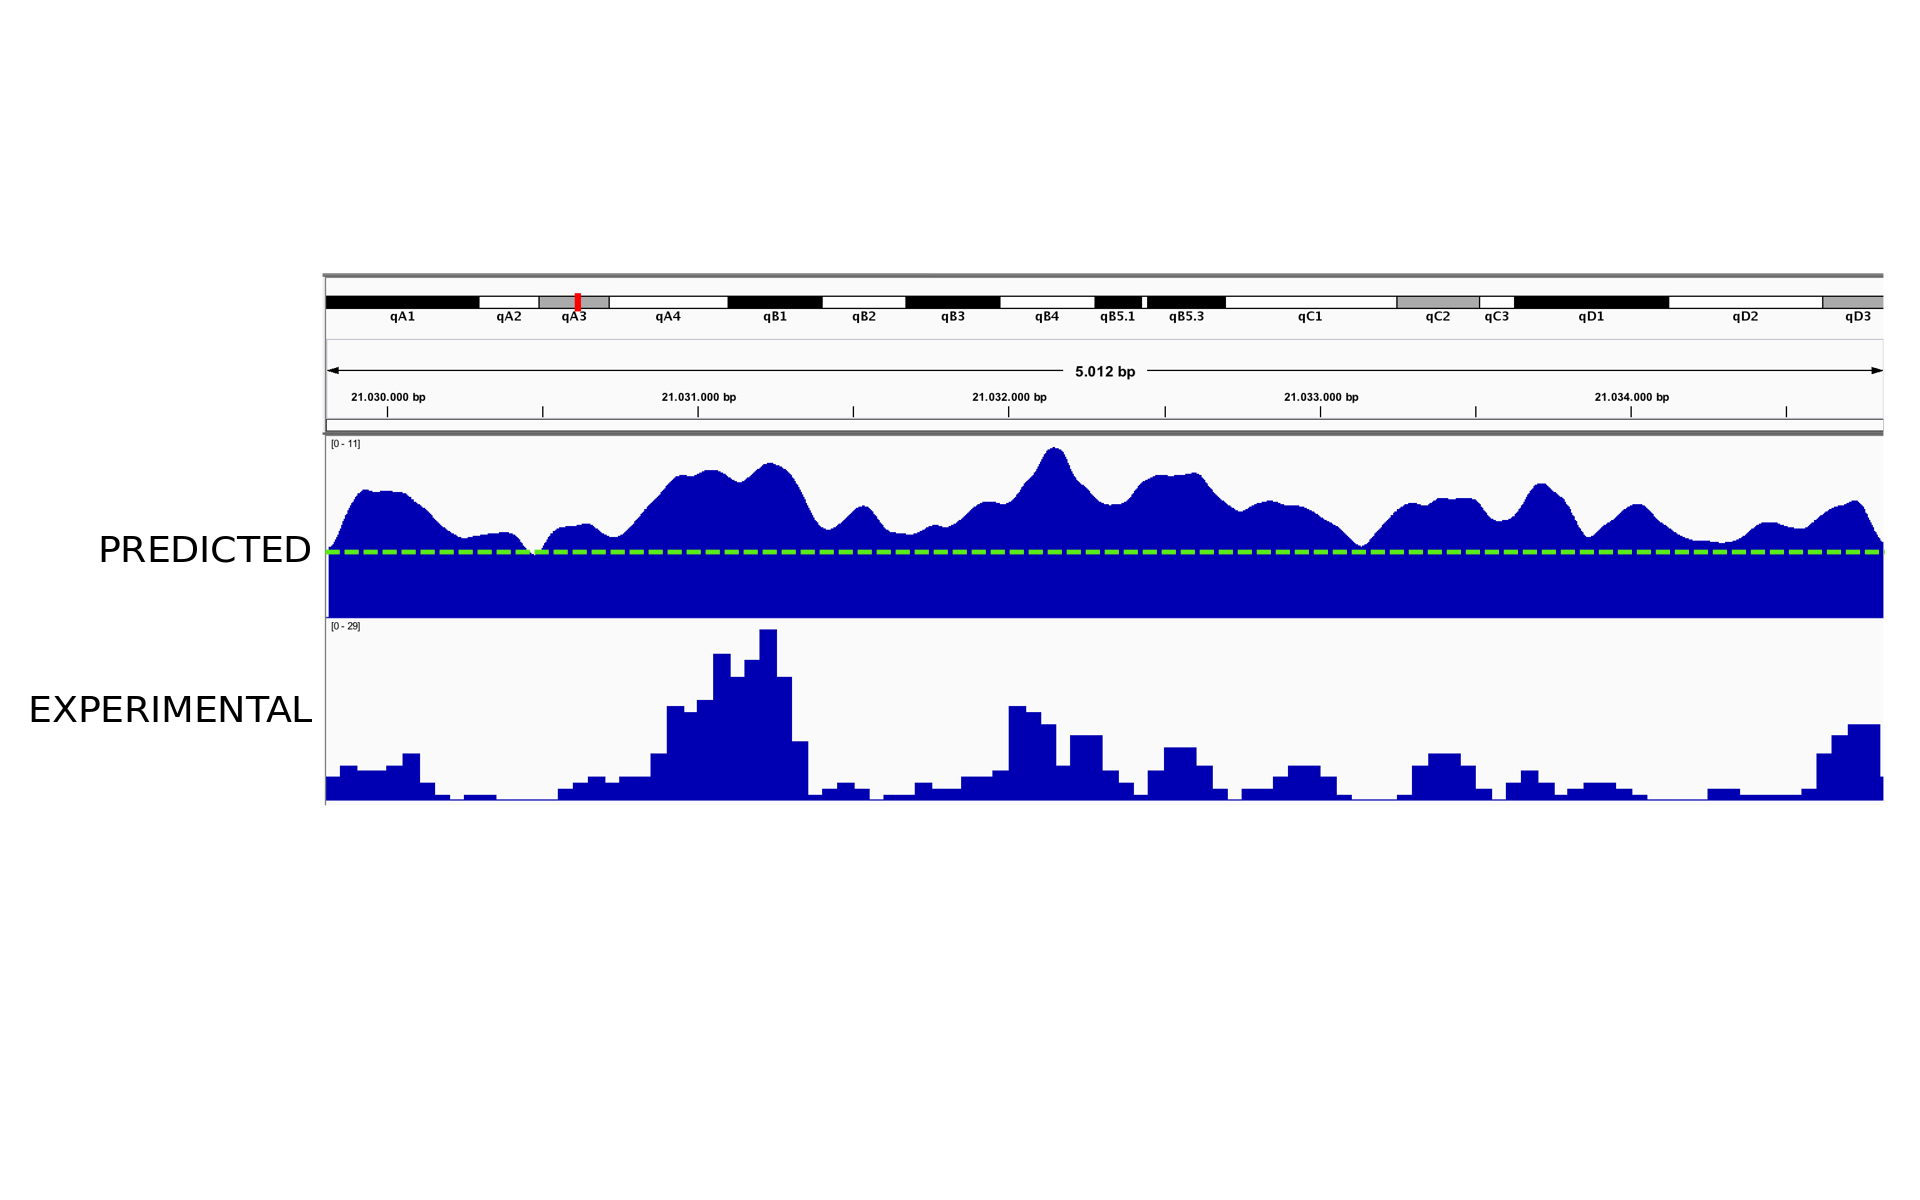
\includegraphics[scale=0.15, trim={0 14cm 0 9cm}, clip]{strand_specific_artcov.png}
%   \end{figure}
%   \onslide<2>{
%   \vspace{-0.4cm}
%   \begin{figure}
%     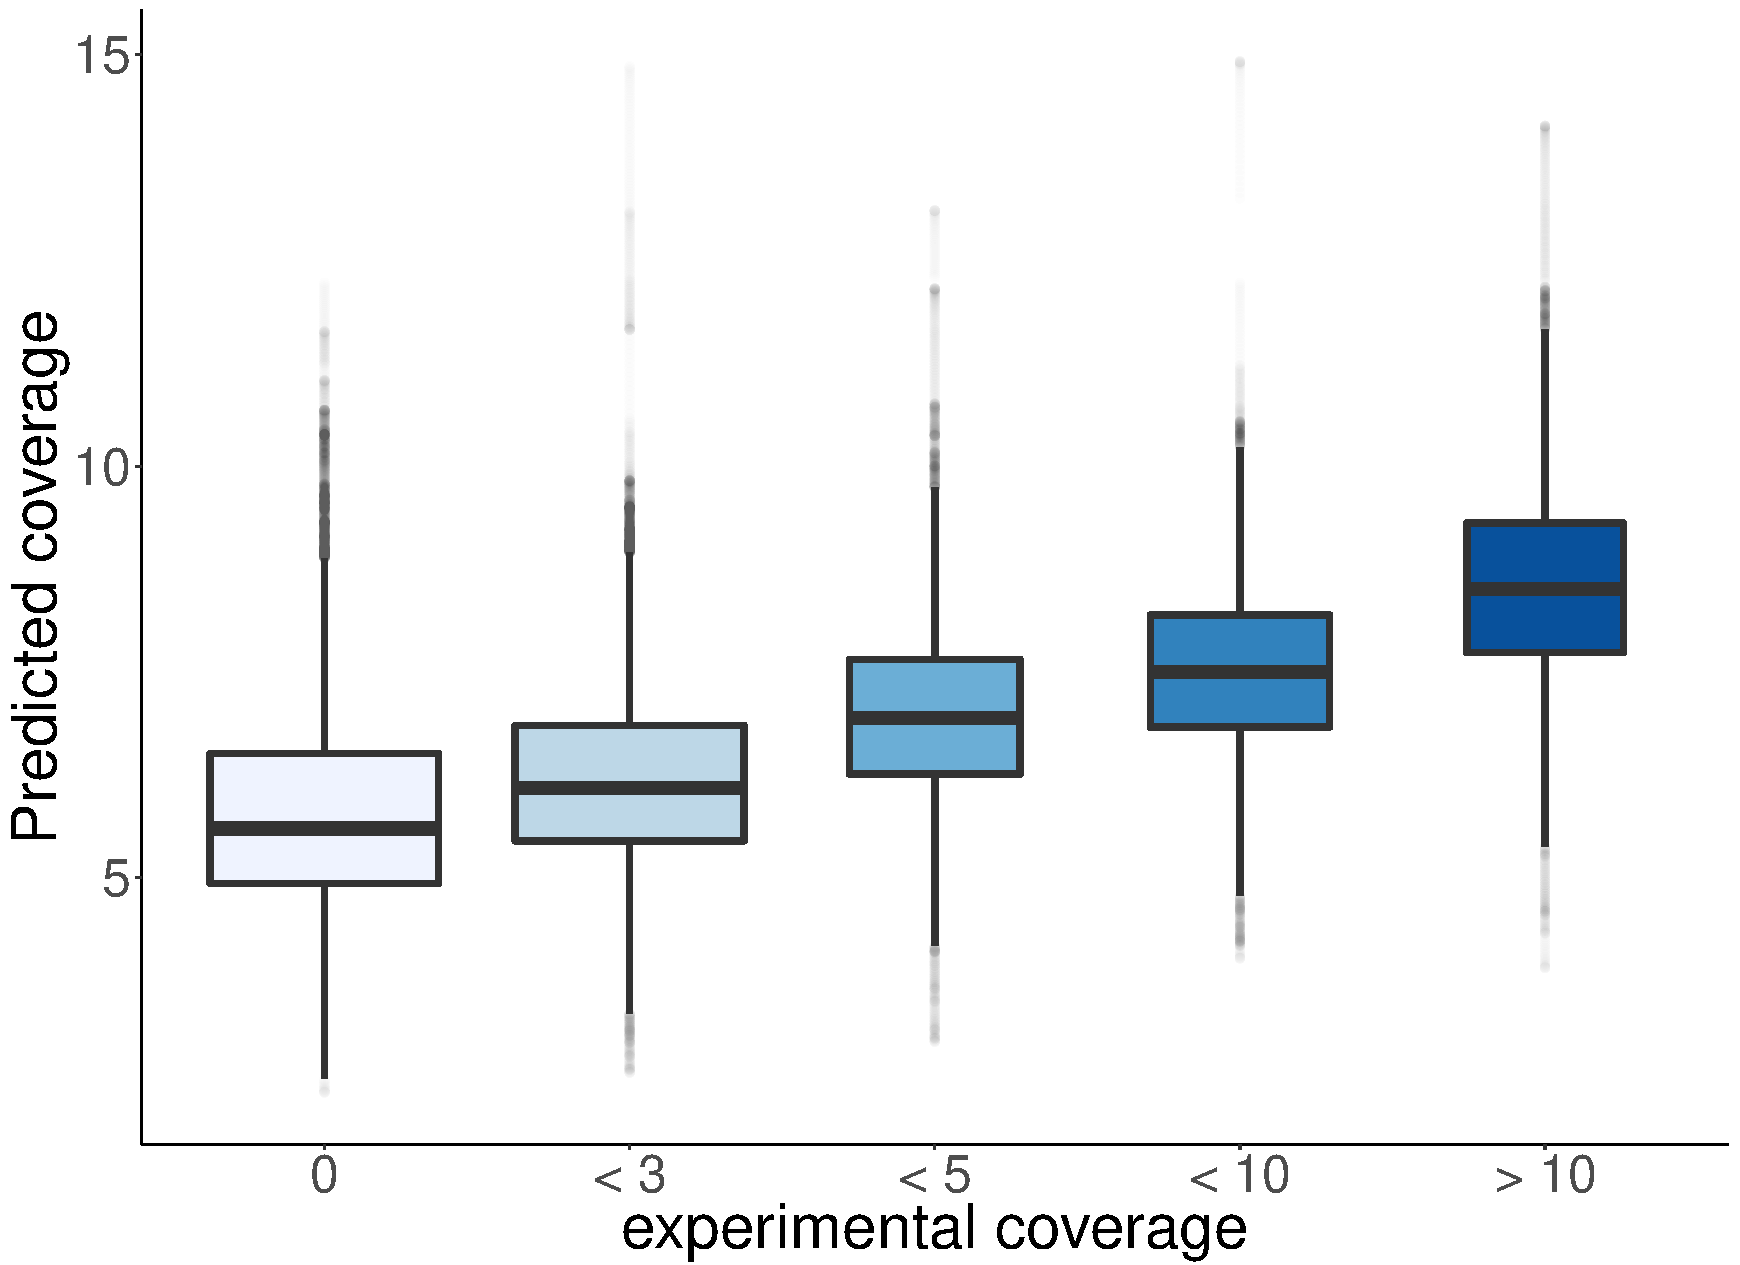
\includegraphics[scale=0.2]{predVSexperimental_boxplot.pdf}
%   \end{figure}
%   }
%   }
% \end{frame}
%
% % \begin{frame}{How much of the bias can be explained by binding events?}
% %   \begin{figure}
% %     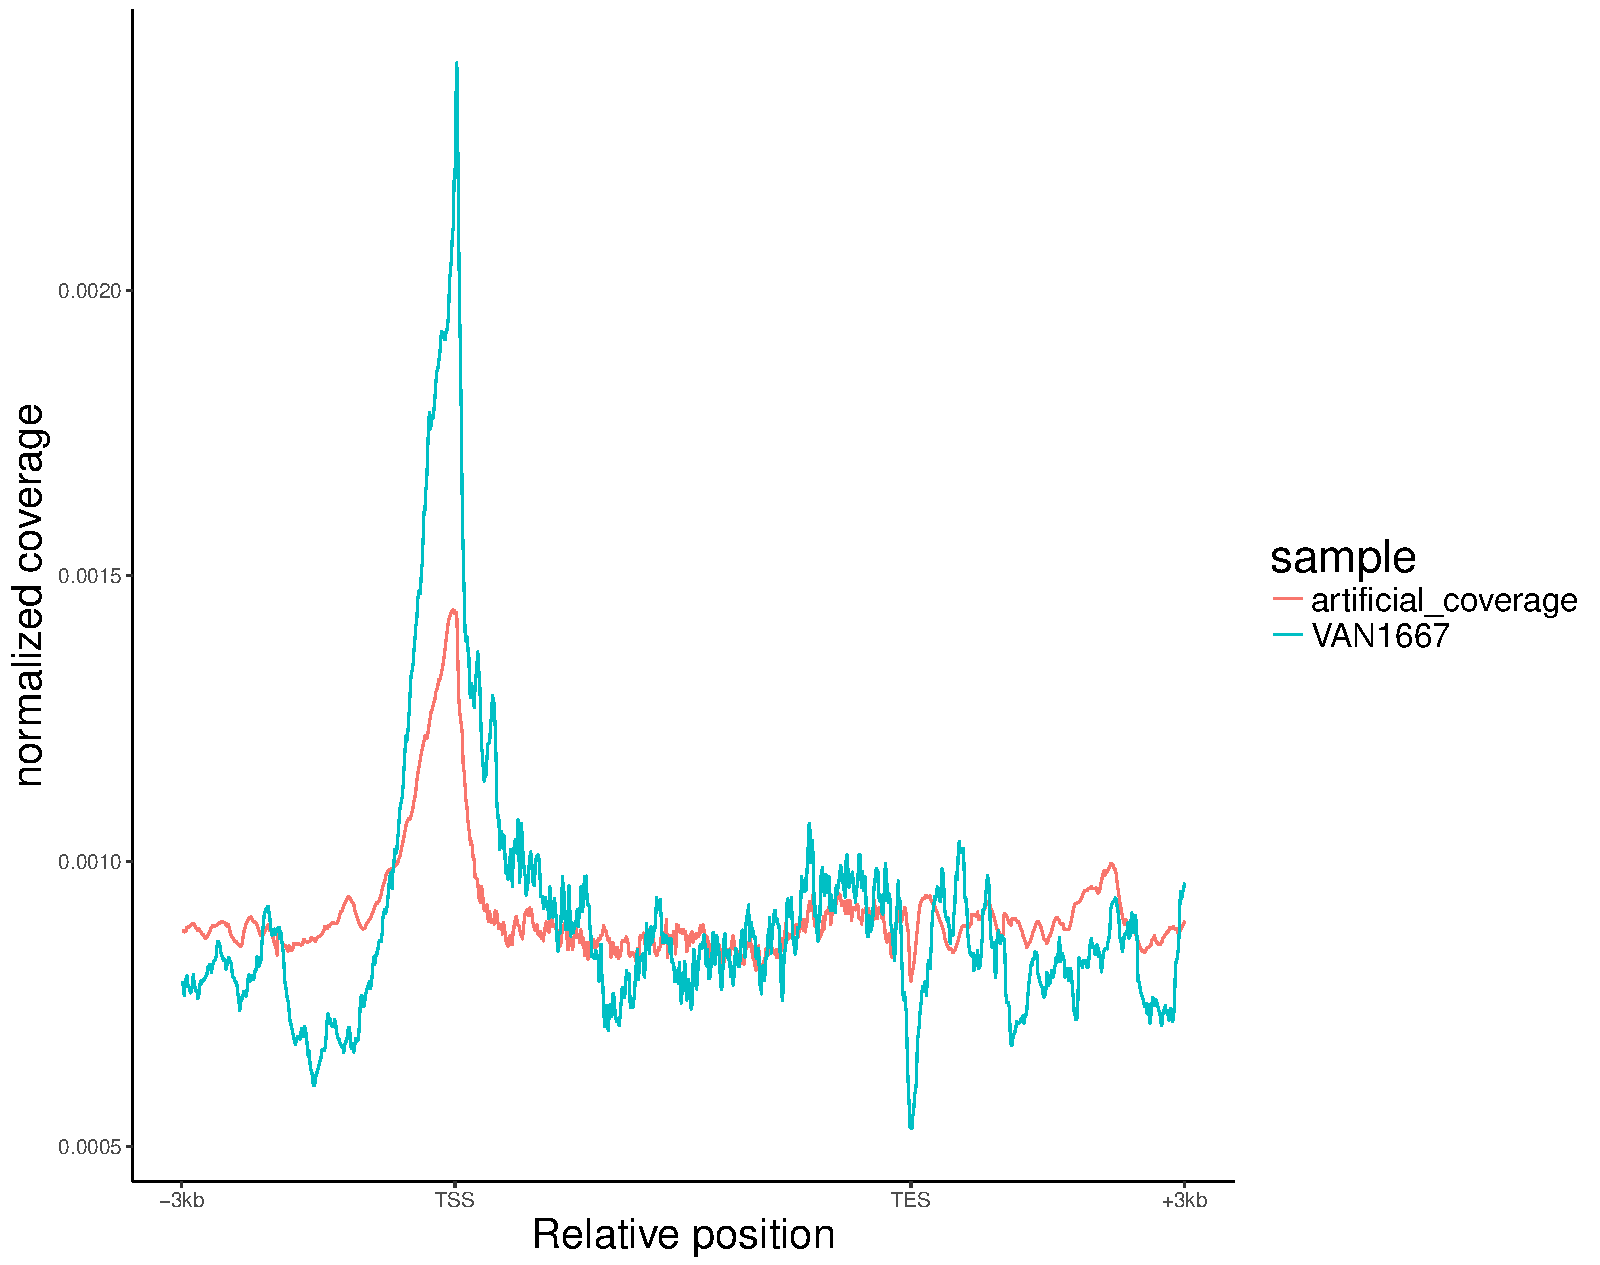
\includegraphics[scale=0.3]{bias_artCovVSVAN1667subsmp.pdf}
% %   \end{figure}
% % \end{frame}
%
% \begin{frame}{Next steps: optimizing the primer pool}
%   \begin{columns}
%   \begin{column}{0.5\linewidth}
%     \begin{itemize}
%       \item Altering the coverage by changing primer concentration
%       \item Finding the optimal primer composition matrix (Differential evolution algorithm)
%     \end{itemize}
%   \end{column}
%   \begin{column}{0.5\linewidth}
%     \animategraphics[scale=0.3, autoplay]{7}{DE_iter-}{1}{99}
%     % \includegraphics{test_iter-1.png}
%   \end{column}
%   \end{columns}
% \end{frame}
%
% \appendix
%
% \begin{frame}{Acknowledgements}
%   \begin{columns}
%     \begin{column}{0.4\linewidth}
%       \begin{itemize}
%         \item \textbf{Alexander Van Oudenaarden}
%         \item \textbf{Christoph Geisenberger}
%         \item \textbf{Anna Alemany Arias}
%         \item Juan Pedraza
%         \item Anna Van Oudenaarden
%         \item Maya Sen
%         \item Lennart Kaester
%         \item Buys de Barbanson
%         \item the AvO lab
%       \end{itemize}
%     \end{column}
%     \begin{column}{0.6\linewidth}
%       \begin{figure}
%         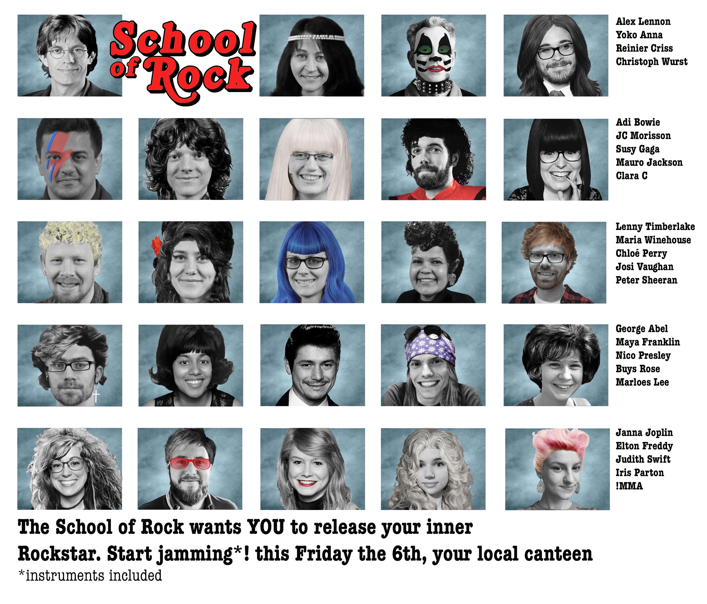
\includegraphics[scale=0.3, trim={0 3cm 3.5cm 0}, clip]{image002.png}
%       \end{figure}
%     \end{column}
%   \end{columns}
% \end{frame}

% \begin{frame}{Ruling out other sources of bias}
% Accessibility
% Primer concentration
% \end{frame}

\end{document}
